\documentclass[11pt]{report}
\usepackage[english]{babel}
\usepackage[utf8]{inputenc}
%\usepackage{citesort} % sorts citation numbers appropriately
\usepackage[]{graphicx} % use this when importing ps- and eps-files
\usepackage{url}
\usepackage{listings}
\usepackage[boxed,linesnumbered]{algorithm2e}
\usepackage{fix-cm}
\usepackage{cite}
\usepackage{verbatim}
\usepackage{enumerate}
\usepackage{fancyvrb}

\usepackage{setspace}
\doublespacing

% \usepackage[pdftex]{graphicx} % use this when importing PDF files

% horizontal margins: 1.0 + 6.5 + 1.0 = 8.5
\setlength{\oddsidemargin}{0.0in}
\setlength{\textwidth}{6.5in}
% vertical margins: 1.0 + 9.0 + 1.0 = 11.0
\setlength{\topmargin}{0.0in}
\setlength{\headheight}{12pt}
\setlength{\headsep}{13pt}
\setlength{\textheight}{625pt}
\setlength{\footskip}{24pt}

\pagestyle{myheadings}

\title{\fontsize{20}{30}\bfseries This is a title}
\author{Flávio Manuel Fernandes Cruz \\}
\date{\today}

\begin{document}
  
\begin{titlepage}

\begin{center}
  
\textsc{\large Flávio Manuel Fernandes Cruz}\\[1.5cm]

\textsc{\LARGE Call Subsumption Mechanisms for Tabled Logic Programs}
\begin{figure}[ht]
  \centering
  
\includegraphics[scale=1.0]{feup.pdf}
\end{figure}


\textsc{\large Faculdade de Engenharia da Universidade do Porto\\ \small Rua Dr. Roberto Frias, s/n \\ 4200-465 Porto PORTUGAL}\\[1.5cm]
  
\end{center}
\end{titlepage}

\addcontentsline{toc}{chapter}{Contents}
\tableofcontents
\listoffigures
\listoftables
\listofalgorithms
\clearpage

\chapter{Introduction}
Logic programming is a very high level programming paradigm that allows the programmer
to focus on the declarative aspects of the problem, instead of describing the specific steps
needed to solve it. Arguably, the Prolog language is the most popular logic
programming language. Part of the success of the Prolog language can be attributed to the
development of a fast and very efficient sequential machine called the \emph{Warren's Abstract Machine}
(WAM) \cite{Warren-83}. The advances in WAM technology and optimization techniques enabled Prolog
to be applied in real world problems in a wide range of fields such as Artificial Intelligence,
Natural Language Processing, Machine Learning, Knowledge Based Systems, Database Management, or
Expert Systems.

While the declarative aspect of Prolog is based on mathematical logic and predicate calculus,
its operational semantics is based one a relatively simple refutation strategy called \emph{Selective Linear Definite}
(SLD) \cite{Lloyd-87}, which is a well defined evaluation method for logic programs that
is particularly well suited to stack based machines.
Furthermore, Prolog defines a few extra-logical constructs, such as the \emph{cut operator}
or the \emph{assertion} facilities that give the programmer more control over the evaluation. Both the SLD operational semantics
and these extra-logical features make the programmer more aware of the actual evaluation process in detriment to the
declarative aspect of the language that is naturally non-deterministic. It is possible to exploit
these deterministic rules to speedup execution or solve
problems related to redundant sub-computations. Notwithstanding, standard Prolog has
still some deficiencies. For instance, writing left-recursive programs can lead to infinite loops.

There have been some attempts in making Prolog less prone to problems related to recursion
and redundant sub-computations, in order to make the language more expressive and closer to
its mathematical logic foundations.
One of these attempts, which is particularly successful, is called \emph{tabling}
(or \emph{tabulation} or \emph{memoization} \cite{Michie-68}). The tabling technique stems from one simple idea:
store intermediate answers in a place called the \emph{table space} and reuse those answers when a
\emph{similar call} appears during the resolution process. Tabling refines the SLD resolution method
by distinguishing between first calls to \emph{tabled subgoals}, which are evaluated as usual through
\emph{program resolution}, and similar calls to tabled subgoals, which are evaluated through \emph{answer resolution}, i.e.,
by consuming answers that are being stored in the table space by the corresponding similar subgoal, instead
of being re-evaluated against the program clauses. Tabled evaluation is able to reduce the search space,
avoid looping, and has better termination properties than traditional SLD resolution \cite{Chen-96}.
The advantages of tabling have lead to its application in fields such as Deductive Databases \cite{Sagonas-94},
Program Analysis \cite{RamakrishnanCR-00}, Knowledge Based Systems \cite{Yang-00}, Inductive Logic
Programming \cite{Rocha-05b}, and Model Checking~\cite{RamakrishnanCR-00}.

In tabling, \emph{call similarity} determines if a subgoal $A$ is similar to a subgoal $B$,
in other words, whether $A$ will generate its own answers or will consume answers from $B$. In general,
we can distinguish between two main approaches for call similarity:

\begin{itemize}
   \item \emph{Variant-based tabling}: $A$ and $B$ are variants if they can be made identical
   through variable renaming as proposed by Bachmair \textit{et al} \cite{Bachmair-93}.
   For example, subgoals \texttt{p(X,1,Y)} and \texttt{p(Y,1,Z)} are \emph{variants},
   because both can be transformed into \texttt{p(VAR0,1,VAR1)};
   \item \emph{Subsumption-based tabling} or \emph{tabling by call subsumption}: Subgoal $A$ is considered similar
   to $B$ if $A$ is \emph{subsumed} by $B$ (or $B$ \emph{subsumes} $A$), i.e., if $A$ is more specific than $B$
   (or an instance of). For example, subgoal \texttt{p(X,1,2)} is subsumed by subgoal \texttt{p(Y,1,Z)} because there
   is a substitution \texttt{\{Y~=~X,~Z~=~2\}} that makes \texttt{p(X,1,2)} an instance of \texttt{p(Y,1,Z)}. Tabling by call
   subsumption is based on the principle that if $A$ is subsumed by $B$ and $S_A$ and $S_B$ are the respective
   answer sets, then $S_A \subseteq S_B$.
\end{itemize}

In general, subsumption-based tabling has the following advantages over variant tabling:
superior time performance, because less program resolution is required; and less space requirements,
as it allows greater reuse of answers, since the answer sets for the subsumed subgoals are not stored.
However, the mechanisms to efficiently support subsumption-based tabling are more complex and harder to
implement, which makes the variant-based tabling approach more popular within the available tabling systems,
such as YapTab \cite{Rocha-00a}, B-Prolog \cite{Zhou-00}, and ALS-Prolog \cite{Guo-01}.
To the best of our knowledge, the SLG-WAM \cite{Sagonas-98} engine from XSB Prolog is the sole tabling system that supports
subsumption-based tabling, initially by using an organization of the table space called
\emph{Dynamic Threaded Sequential Automata (DTSA)}~\cite{Rao-96}, and later by using an alternative design called
\emph{Time Stamped Tries (TST)}~\cite{Johnson-99}, which is a simpler approach and uses far less memory.

\section{Thesis Purpose}

In this thesis we address the design, implementation, integration and evaluation of two subsumption-based engines
built on top of YapTab \cite{Rocha-00a}, the tabling system that is part of Yap Prolog. For the first engine, we
reused and integrated the Time Stamped Tries approach from SLG-WAM into YapTab.
We studied how subsumption-based and variant-based tabling were seamlessly
integrated into the SLG-WAM engine and we attempted to reuse most of the original code and data structures when
integrating these new mechanisms into YapTab.  Consequently, we made minimal modifications to the YapTab engine
that enabled it to support a mix of variant and subsumptive subgoals on the same program.
Our performance results show that our integration efforts were successful, with comparable
speedups to the SLG-WAM when using subsumptive-based tabling against variant-based tabling.

For the second system, we designed a novel extension for subsumptive-based tabling called
\emph{Retroactive Call Subsumption} (RCS).
This extension attempts to solve one major problem in traditional call subsumption: the order in
which subgoals are called during a particular evaluation can greatly affect the success and applicability
of the call by subsumption technique. For example, if more specific subgoals are called before
the more general subgoal, no reuse will be employed, while if the more general subgoal is called first,
reuse will happen. The RCS extends the original TST design by allowing full sharing of answers, independently
of the order they are called. The basic idea is to selectively prune and restart the evaluation of generator
subgoals that are subsumed by a new called subgoal in order to reuse the answers from the subsuming subgoal,
instead of continuing to generate their own answers.

To implement retroactive-based tabling we developed a few novel ideas: (1) a novel algorithm to efficiently
traverse the table space data structures and retrieve the running \emph{instances} of a subgoal; (2) a novel table
space organization, based on the ideas of the \emph{common global trie} proposal~\cite{CostaJ-08}, where answers
are represented only once; and (3) a new evaluation strategy capable of pruning and transforming generator nodes
into consumer nodes.

Our results show that the overhead of the new mechanisms for RCS support are low enough in programs that do not
benefit from it, which, combined with considerable gains for programs that can take advantage of them, validates
this new evaluation technique. With this in mind, we argue that Retroactive Call Subsumption makes tabling
more adapted and useful for practical applications and is another great functionality in the programmer's toolbox for
writing tabled logic programs.

\section{Thesis Outline}

In the following list we describe each chapter of this thesis.

\begin{description}

   \item[Chapter 1: Introduction.] Is this chapter.
   
   \item[Chapter 2: Logic Programming and Tabling.] Provides an overview of the main topics of this thesis.
   The subjects discussed are logic programming, Prolog, and tabling for logic programs. A brief description
   of the YapTab and SLG-WAM tabling engines is also presented.
   
   \item[Chapter 3: Table Space Organization.] Describes the table space organization for both variant and
   subsumption-based tabling engines. We start by describing the variant table space for both SLG-WAM and
   YapTab systems. We then give a brief overview about the table space organization for the DTSA and TST
   techniques that implement tabling with subsumptive checks.
   
   \item[Chapter 4: Time Stamped Tries.] Throughly presents the Time Stamped Tries approach to subsumption-based
   tabling. First, we describe the algorithm used to detect subsuming subgoals. Next,
   we give a detailed description of the data structures used in the table space that are used to speedup
   the identification of relevant answers for subsumed subgoals. Finally, we focus on the modifications we have
   made to the YapTab tabling engine in order to support tabling by call subsumption based on the TST approach.
   
   \item[Chapter 5: Retroactive Call Subsumption.] We start with the motivations behind RCS, by showing the shortcomings
   of pure subsumption-based tabling. We next describe the rules for the new mechanism and the problems that arise
   when pruning execution branches. Finally, we discuss the novel table space organization called \emph{Single Time
   Stamped Trie} (STST) and then we throughly describe the new algorithm developed to find executing subsumed subgoals
   of a subgoal on the table space.
   
   \item[Chapter 6: Experimental Results.] This chapter first presents the experimental results we achieved with
   the new YapTab engine that reuses the TST approach and how it compares to the SLG-WAM. We also make a space
   analysis comparison between call subsumption and variant-based tabling.
   Next, we present and discuss the overhead of the RCS mechanism on programs that do not benefit from it and
   the speedups we have achieved for programs that can take advantage of it. Finally, we present an analysis of
   the STST table organization by experimenting with programs that stress the nature of this table space organization.
   
   \item[Chapter 7: Conclusions.] Summarizes the work, enumerates the contributions and suggests directions for
   future work.
   
\end{description}


\chapter{Logic Programming and Tabling}

The purpose of this chapter is to give an overview of the research areas
involved in this dissertation. First we explain the fundamental ideas of logic
programming and Prolog; next, tabling by call variance is described, focusing on
the execution strategy and data structures; finally, tabling by call subsumption
and related strategies like \textit{time stamped tries} are explained.

\section{Logic Programming}

Logic programming presents a declarative style of programming based on mathematical
logic and the predicate calculus. It is a very high level programming
paradigm that allows the programmer to focus on the problem at hand, leaving the
steps on \textit{how} to solve the problem to the computer.

In its purest form, logic programming is solely based on Horn Clause Logic \cite{Lloyd-87},
a subset of First Order Logic. Programming in logic can be viewed as
a two step process: (1) first, the theory is formulated as logic clauses,
next (2) we use this theory to search for alternative ways in which an arbitrary query is satisfied.

Logic programming is often mentioned to include the following advantages \cite{Carlsson-PhD}:

\begin{itemize}
  \item \textbf{Simple declarative semantics}: a logic program is simply a collection of predicate logic clauses.
  \item \textbf{Simple procedural semantics}: a logic program can be read as a collection of recursive procedures. In Prolog, for instance, clauses are tried in the order they are written and goals within a clause are executed from left to right.
  \item \textbf{High expressive power}: Logic programs can be seen as executable specifications that despite their simple procedural semantics allow for designing complex and efficient algorithms.
  \item \textbf{Inherent non-determinism}. Since in general several clauses can match a goal, problems involving search are easily programmed in these kind of languages.
\end{itemize}

\subsection{Logic Programs}

A logic program is composed by a set of Horn clauses. Each clause is a disjunction of literals
and contains at most one positive literal. Horn clauses are usually written as

\begin{center}
  $L_{1}, ..., L_{n} \Longrightarrow L  (\equiv \neg L_{1} \vee ... \neg L_{n} \vee \neg L)$
\end{center}

or

\begin{center}
  $L_{1}, ..., L_{n}  (\equiv \neg L_{1} \vee ... \neg L_{n})$
\end{center}

where $n >= 0$ and $L$ is the only positive literal. 

A Horn clause that has exactly one positive literal is called definitive clause; in the Prolog language
it is usually called a \textit{rule}.
A Horn clause without a positive literal is called a \textit{goal}.

Using Prolog's notation, one can write \textit{rules} in the form

\begin{center}
  $L :- L_{1}, ..., L{n}.$
\end{center}

Usually, $A$ is called the \textit{head} of the \textit{rule} and $L_{1}, ..., L_{n}$
the \textit{body} of the \textit{rule}, where each $L_{i}$ is called a subgoal.
A logical \textit{fact} is a special \textit{rule} where the \textit{body} is replaced by \textit{true} symbol:

\begin{center}
  $L.$
\end{center}

Goals are \textit{rules} without the \textit{head} component and are also named as \textit{queries}.


Each literal in Horn clause has the form $p(t_{1}, ..., t_{n})$, where $p$ is the \textit{predicate} symbol or \textit{functor}
and each $t_{i}$ are \textit{terms}. A term can be a \textit{constant} (or \textit{atom}), a \textit{variable}
or a \textit{compound} term. Compound terms follow the predicate structure, recursively.
Variables are assumed to be universally quantified and have the following major characteristics:

\begin{itemize}
  \item Variables are logical variables that can instantiated only once.
  \item Variables are untyped until instantiated.
  \item Variables are instantiated via \textit{unification}, a pattern matching operation that finds the most general common instance of two data objects. 
\end{itemize}

A sequence of clauses with the same functor in the head form a \textit{predicate}. The ordering
of these clauses can have some implications depending on the resolution semantics of the underlying language.
Prolog for instance, uses a top-down resolution mechanism known as \textit{SLD} (Selective Linear Definite) resolution \cite{Lloyd-87}.

SLD starts by matching the first subgoal query to the first clause of the respective predicate,
generating a new query using the body of the clause, which is added to the remaining query subgoals.
During this process a finite set of pairs $\theta$ called \textit{substitution} is built.
Each pair has the form $X = t$, where $X$ is a variable and $t$ is a term. No variable in the left-hand side
of a pair appears on the right-hand side and no two pairs have the same variable as left-hand side \cite{Sterling-94}. 
When the clause body is reused as query, all the variables present in the terms are replaced using the
set $\theta$. 

If unification fails, the next clause of the predicate is tried, in a mechanism called \textit{backtracking}.
This recursive computation fails when there are any more clauses left to try. It succeeds when the subgoal query is empty.

The resolution process is fundamentally non-deterministic and can be viewed as a search within a tree. SLD
does not force any specific search strategy for exploring the tree. Prolog for example, uses a depth-first, one
branch at a time search.

\subsection{Prolog and WAM}
  
Prolog is one of the first logic programming languages and arguably the most successful.
The first implementation of Prolog was Marseille Prolog, developed in 1972 by Alain Colmerauer and Robert Kowalski \cite{Kowalski-74}.

The use of Prolog as a practical and efficient language was made viable by David Warren in 1977, when he built a compiler that could
compete with other languages like Lisp \cite{Warren-77}. Then in 1983, David Warren formulated an abstract machine known as WAM
(\textit{Warren Abstract Machine}) \cite{Warren-83} that is still widely used in modern Prolog implementations.

\subsubsection{Prolog}

Prolog follows the semantics of the SLD resolution through a depth first search strategy.
It starts by choosing the top-most clauses of the predicate and the subgoals are solved
within a left-to-right fashion.

For illustration purposes, we defined the factorial predicate (Listing \ref{factorial_prolog}) that can compute the factorial of
any given number. This predicate has arity of 2, where the first argument is an \textit{input} argument and the second argument
an \textit{output} argument.

\begin{lstlisting}[language=prolog,basicstyle=\footnotesize,float,frame=single,caption={Factorial function in Prolog.},label=factorial_prolog]
factorial(0, 1) :- !.
factorial(N, R) :-
  N > 0,
  N1 is N - 1,
  factorial(N1, R1),
  R is R1 * N.
\end{lstlisting}

Factorial is composed of two clauses, one represents the factorial base case (factorial of 0 is 1) and
the other represents the recursive relation. The second clause first checks if the input number
is positive, to discard non-positive numbers, then computes $N - 1$ and recursively
calls factorial to compute the value of $factorial(N-1)$, finally, the variable $R$ is then unified
to $N * factorial(N-1)$. The first clause uses the \textit{cut} operator that tells the Prolog engine to not explore alternative
clauses, i.e., the factorial of 0 is not to be computed with the recursive relation declared on the second clause.

\begin{figure}[ht]
  \centering
    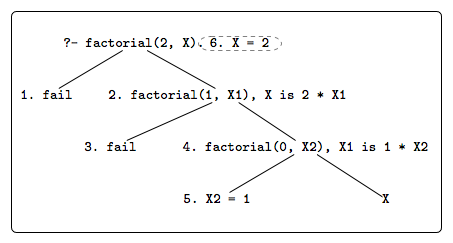
\includegraphics[scale=0.6]{factorial.png}
  \caption{Factorial search tree.}
  \label{fig:factorial_tree}
\end{figure}

Once Prolog finds the first solution (Figure \ref{fig:factorial_tree}), the cut control operator disables further
alternatives, completing the depth first search in the tree.

The cut operator is not the only special instruction in Prolog, more built-in predicates are also available:

\begin{itemize}
  \item \textbf{Meta-logical predicates}: inquire the state of the computation and manipulate terms.
  \item \textbf{Extra-logical predicates}: they can manipulate the Prolog database, adding or removing clauses from
  the program being executed. Input/Output operators are another example of extra-logical predicates.
  \item \textbf{Other predicates}: predicates to perform arithmetic operations, to compare terms, to support debugging, etc.
\end{itemize}

These special operators make programming more practical and useful in real world applications.

\subsubsection{WAM}

The WAM is an abstract machine based on a stack-based architecture with various data areas, registers, and low level instructions
that can be efficiently executed, manipulated and optimized.

The WAM uses the following execution stacks:

\begin{itemize}
  \item \textbf{Code Area}: Contains the compiled instructions.
  \item \textbf{PDL}: A push down list used by the unification process.
  \item \textbf{Trail}: Stores the addresses of the variables that must be reset when backtracking.
  \item \textbf{Stack}: Stores \textit{environment} and \textit{choice point} frames. Environments track the flow control in a program
  and choice points store open alternatives, which are used to restore the state of the computation when backtracking.
  \item \textbf{Heap}: Array of data cells used to store variables and compound terms that cannot
  be stored in the stack.
\end{itemize}

For the registers, WAM defines the following:

\begin{itemize}
  \item \textbf{S}: used during the unification of compound terms.
  \item \textbf{HB}: it is set to contain the value of the register \textbf{H} at the time of latest choice point. This is used to
  determine \textit{conditional} variable bindings that affect variables existing before the creation of the choice point.
  \item \textbf{P}: points to current WAM instruction.
  \item \textbf{CP}: stores the value of \textbf{P} before the current invoked call and it is used to restore the execution point.
  \item \textbf{TR}: points to the top of the trail stack.
  \item \textbf{E}: points to the current active environment.
  \item \textbf{B}: the active choice point.
  \item \textbf{H}: points to the top of the heap stack.
\end{itemize}

WAM instructions can be grouped into four main groups: choice point instructions to manipulate choice points; control
instructions to manage environments and control the execution flow; unification instructions that implement
specialized versions of the unification algorithm; and indexing instructions to efficiently determine which clauses
unify with a given subgoal call.

The WAM being a complex topic has complete books dedicated in explaining its intricacies.
An example is the \textit{Warren's Abstract Machine -- A Tutorial Reconstruction} written by H. A\"{\i}t-Kaci \cite{Aitkaci-91}. 

\section{Tabling}

Despite Prolog's declarativeness and expressiveness, the past few years have seen wide efforts at
solving shortcomings that arise when using SLD resolution.
One proposal that has gained popularity is \textit{tabling} or \textit{tabulation} \cite{Chen-96}.
In comparison to the traditional resolution method, tabling can reduce the search space to cut redundant computations,
avoids looping and has better termination properties \cite{Tamaki-86}.

In a nutshell, tabling is a refinement of the SLD resolution that consists in storing intermediate answers for
subgoals so that they can be reused when a repeated subgoal appears in the resolution process.
The use of tabling enables the programmer to write more expressive, but still valid, logical clauses.

One classical example that is used to demonstrate the need of tabling is presented in Listing \ref{prolog_path}.
This program describes the predicate \textbf{path/2} that can compute reachability between two nodes on a directed graph.
Connections are established as facts using the \textbf{edge/2} predicate.

\begin{lstlisting}[language=prolog,basicstyle=\footnotesize,float,frame=single,caption={\textit{path} program.},label=prolog_path]
:- table path/2.

path(X, Z) :- edge(X, Y), path(Y, Z).
path(X, Z) :- edge(X, Z).

edge(a, b).
edge(b, a).
\end{lstlisting}

\begin{figure}[ht]
  \centering
    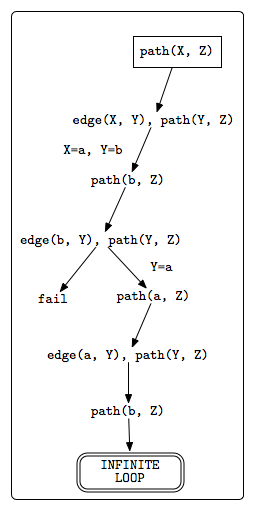
\includegraphics[scale=0.5]{infinite_loop.png}
  \caption{Infinite loop evaluating \textbf{path(X, Z)}.}
  \label{fig:infinite_loop}
\end{figure}

If we tried to evaluate the query goal \textbf{?- path(X, Z).}, traditional Prolog would enter an infinite loop (Figure \ref{fig:infinite_loop})
because the first clause of \textbf{path/2} is right recursive, leading to a repeated call.

\subsubsection{Tabling evaluation}

In this new method of evaluation when a tabled subgoal is first called, a new entry is allocated on the \textit{table space}. Table
entries are used to store subgoal calls but they also store answers found during evaluation. Each time a tabled subgoal is called, we
know if it is a repeated call by inspecting the table space. Nodes in the search space can be classified as:
\textit{generator nodes}, if they are being called for the first time; \textit{consumer nodes} if they are repeated calls;
or \textit{interior nodes} if they are non-tabled subgoals. Generator nodes are matched against the predicate clauses as usual but
consumer nodes are not, instead they consume answers stored in the table space from the respective subgoal.

In Figure \ref{fig:tabling_path} we depict the tabled evaluation of \textbf{?- path(X, Z).}.
Generator nodes are represented by rectangles with double lines and consumer nodes by simple rectangles.
Note that we apply to \textbf{path/2} the \textbf{table} directive to use tabling resolution.

Tabled evaluation starts by inserting a new entry in the table space and by allocating a generator
node to represent \textbf{path(X, Z)} (step 1). Like SLD, \textbf{path(X, Z)} is resolved against the first \textbf{path/2} clause (step 2).
The goal \textbf{edge(X, Y)} is not tabled and is resolved as usual. We use the first \textbf{edge/2} clause with $X = a, Z = b$
and these values are carried to \textbf{path(b, Z)} (step 3). This goal is not yet in the table space, hence we add a new entry for it.

\textbf{path(b, Z)} is then resolved against the first clause of \textbf{path/2} (step 4). \textbf{edge(b, Y)} fails against the first clause but succeeds
with $Y = a$. A new tabled subgoal \textbf{path(a, Z)} is registered in the tabled space (step 6) and resolved against the first clause
of \textbf{path/2} (step 7). This time the \textbf{edge/2} subgoal matches with the first clause ($Y = b$). A repeated tabled subgoal
\textbf{path(b, Z)} is called and the first consumer node is allocated (step 8). As we have no answers for \textbf{path(b, Z)} to consume,
the current evaluation point is \textit{suspended}. Later on, this node can be resumed to consume new answers.

Next, we backtrack to node 7 and try the second \textbf{edge/2} clause, but resolution fails (step 9). We backtrack again, this time to
node 6 to try the second clause of \textbf{path/2} (step 10). Here \textbf{edge(a, Z)} is resolved against the first clause of \textbf{edge/2}
and the solution $Z = b$ is found for the subgoal \textbf{path(a, Z)}. This solution is stored in the table space and forward
execution, propagating the binding $Z = b$ to \textbf{path(b, Z)} (step 12) and the first solution to this subgoal is found and stored.
We continue forward execution and the binding is once again propagated, this time to node 3 (step 13) and we find a solution to
\textbf{path(X, Z)}, $X = a, Z = b$.

\begin{figure}[ht]
  \centering
    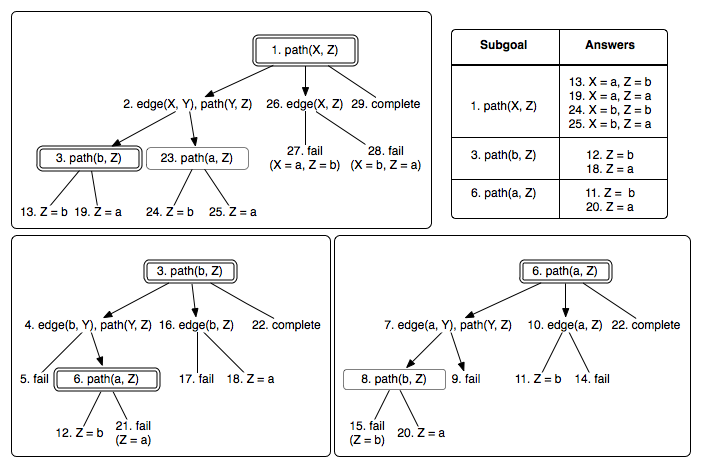
\includegraphics[scale=0.6]{tabling_path.png}
  \caption{Tabled evaluation of \textbf{path(X, Z)}.}
  \label{fig:tabling_path}
\end{figure}

We return to node 10 to try the second clause of \textbf{edge/2}, but we fail (step 14). With no more clauses to try at node 6,
we check wether consumer in node 8 can be resumed. It can, as now it has one unconsumed answer. We resume computation on node 8,
the answer $Z = b$ is consumed and forwarded to subgoal \textbf{path(a, Z)} at node 6. Here, we note that it is a repeated answer
to this subgoal by inspecting the table space, and thus we mark step 15 as \textbf{fail}. Failing repeated answers is crucial
to avoid unnecessary computations and sometimes looping.

At this point, we return again to node 6 but no consumers with unconsumed answers exist and the subgoal cannot be \textit{completed}.
Completing \textbf{path(a, Z)} earlier is not safe, because the consumer under it depends on generator node 3, the subgoal \textbf{path(b, Z)}.
If new answers are found, node 8 should be resumed to consume them, which then can lead to new answers for \textbf{path(a, Z)}.
Completing prematurely would result in lost answers.

We thus backtrack to node 3
to try the second clause (step 16). The first clause of \textbf{edge/2} fails but the second succeeds (step 18), culminating in
a new answer for \textbf{path(b, Z)}, $Z = a$, that is stored. We propagate variable bindings in step 19, generating a new answer
to subgoal \textbf{path(X, Z)}, $X = a, Z = a$.

Every clause in generator node 3 has been tried, so we check if it can be completed. Note that we can safely complete this node,
as it is the youngest generator in which younger consumer nodes have no dependencies on older generator nodes.
Node 3 is called, by definition, a \textit{leader node} and the branch of nodes
below it form a \textit{Strongly Connected Component} (SCC) \cite{Tarjan-72}.

When trying to complete node 3, we verify that node 8 has unconsumed answers. The answer $Z = a$ is fetched (step 20) and propagated
to node 6, generating a new answer to \textbf{path(a, Z)}. This binding is once again propagated, now for node 3 (step 21) but it is
a repeated answer, thus the computation fails. We return back to node 3 to re-attempt completion. This time, no consumers have unconsumed
answers and we can safely complete (step 22). Subgoals \textbf{path(b, Z)} (node 3) and \textbf{path(a, Z)} (node 6) are marked as \textbf{complete}
in the table space and no new answers are accepted.

Next, we backtrack to node 2 to try the second \textbf{edge/2} clause. A new consumer node is allocated (step 23) and answers can be
promptly consumed from the table space. As the subgoal \textbf{path(a, Z)} as been completed before, the consumer node is thus deallocated.
The retrieved answers in step 23 are propagated to node 1 and new answers are generated (step 24 and 25).

We backtrack to node 1 to try the second \textbf{edge/2} clause. Resolution succeeds for both clauses but as the newly found answers
are repeated we fail for both cases (step 27 and 28). The process backtracks again to node 1 and with no more clauses to try,
we attempt completion. As there are no consumer nodes, completion is done (step 29) and computation terminates successfully.

From the described example we can summarize four main operations needed to support tabled evaluation:

\begin{itemize}
  \item The \textit{tabled subgoal call} operation represents a call to a tabled subgoal.
  If the subgoal is already in the tabled subgoal it creates a new consumer node to consume answers.
  If it is a new subgoal call it creates a new generator node and adds a new entry to the table space.
  Each new entry contains an empty set $S$ that will contain answers for the subgoal. 
  
  \item The \textit{new answer} operation adds a new answer $s$ to the table space. If the answer is repeated the operation fails.
  A new answer set $S'$ for the subgoal is generated: $S' \equiv S \cup {s}$.
  
  \item The \textit{answer resolution} operation checks wether new answers from the table space are available for consumption.
  When no new answers are available, the consumer node is \textit{suspended} and execution proceeds using a specific strategy.
  Given the last consumed answer, we determine the unconsumed answer
  set $R$ ($R \subseteq S$) and fetch the element $r \in R$, which is the first element from the set $R$. The last consumed answer
  can be seen as a \textit{continuation} that is stored in each consumer node and is used to determine the next available answer.
  
  \item The \textit{completion} operation determines if a tabled subgoal is \textit{completely evaluated}.
  Only leader nodes can complete themselves and younger generator nodes.
  Once a subgoal is completed the set of answers $S$ is closed and no more answers are accepted; future subgoal calls
  can use the set $S$ without the need to suspend.
\end{itemize}

\subsubsection{Scheduling strategies}

Ensuring efficient execution of tabled evaluation requires different \textit{scheduling strategies}.
During evaluation of the previous example it is very clear that at several points we can choose between
different strategies: continue forward execution, backtrack to interior nodes,
return answers to consumer nodes, or perform completion. Depending on how and when the return of answers is scheduled, different
strategies and searches can be formulated. It is also well known
that using different strategies leads to tremendous effect on performance as some predicates are better suited to specific strategies. 
The most popular scheduling strategies are batched scheduling and local scheduling \cite{Freire-96}.

\textit{Batched scheduling} reduces the need to suspend and move around the search tree by batching the return of answers.
When the engine generates answers, while evaluating a particular goal, the answers are added to the table and the subgoal continues its normal
evaluation until it resolves all available program clauses. Only then the answers are consumed by consumer nodes \cite{Freire-96}.
In some cases, this results in creating dependencies to older subgoals, therefore enlarging the current SCC and delaying completion
to older generator nodes. When backtracking, three situations may arise:

\begin{itemize}
  \item if backtracking to a generator or interior node, try the next available clause.
  \item if backtracking to a consumer node, consume new answers.
  \item if no more clauses are left to try or no more unconsumed answers are available, two options are available:
    \begin{itemize}
      \item if the node is a leader node, attempt completion.
      \item if not, backtrack to a previous branch.
    \end{itemize}
\end{itemize}

For some problems, \textit{local scheduling} is better suited because it tries to evaluate a single exact SCC at a time, preserving the dynamic
SCC ordering during the evaluation. In other words, in a local evaluation, answers are returned to consuming nodes outside of an SCC only after that
SCC is completely evaluated \cite{Freire-96}.
It differs from batched scheduling in that once the answers are found, they are added to the table space, but execution
\textit{fails}. Because this strategy tries to complete sooner rather than later, we can expect less dependencies between subgoals.

\subsubsection{Variant tabling} \label{sec:variant_tabling}

When the subgoal \textbf{path(X, Z)} is called, a check for the presence of this subgoal in the table space is done first.
In the example in Figure \ref{fig:tabling_path}, this was done by checking wether a \textit{variant} of the new goal already
exists in the table. We say that two terms $t_1$ and $t_2$ are variants of each other if they are identical up to renaming of their
variables.

For example, \textbf{path(X, Z)} is variant of the subgoal \textbf{path(X, Y)}, as they represent the same subgoal if we try
to rename their variables to a standardized format. One format was proposed by Bachmair \textit{et al} \cite{Bachmair-93}. Formally,
we have a set $V$ of variables present in a term and a function $renameVar$, such that the first term variable $a \in V$
results in $renameVar(a) = VAR0$ and the following distinct variables are named incrementally ($VAR1, VAR2, ...$).
Using this mechanism, \textbf{path(X, Z)} and \textbf{path(X, Y)} results in \textbf{path(VAR0, VAR1)}. The resulting
standardized subgoal is then checked against the table space to verify if it is a repeated subgoal call.

The variant approach is widely used in tabling systems, but other approaches do exist. One approach named
\textit{call by subsumption} works by checking wether the new goal is subsumed by another goal in the table space.
In other words, we verify if there is a more general subgoal than the one being called. For example
\textbf{path(b, Z)} is subsumed by the subgoal \textbf{path(X, Z)}.

In this approach, instead of creating
a new generator node in step 3, we create a consumer node that would consume answers stored in the subgoal \textbf{path(X, Z)}.
For correct results, it should be clear that the answers used from the table space must unify with \textbf{path(b, Z)}.
Like variant tabling, those new consumer nodes do not expand by using the program clauses, hence the search tree for this new
method will be greatly reduced. This new approach will be throughly explored in Section \ref{sec:subsumption} (Tabling by Call Subsumption).

  \subsection{Yap and XSB}
  
  Yap \cite{system-yap} and XSB \cite{system-xsb} are two well known Prolog systems that implement tabling.
  
  The YAP Prolog System is a high-performance Prolog compiler developed at LIACC, Universidade do Porto.
  It is one of the fastest available Prolog systems and implements a wide range of functionalities: 
  stream I/O, sockets, modules, exceptions, debugging, a C-interface, dynamic code, internal database, DCGs, saved states, co-routining, arrays and threads.
  It is based on the WAM and follows the Edinburgh tradition. Most of the ISO-Prolog standard is implemented.
  
  Tabling in Yap is implemented through the YapTab sub-system \cite{Rocha-00a}, a delaying based tabling engine supporting evaluation of
  definite programs. YapTab follows the seminal SLG-WAM (Linear resolution with Selection function for General logic programs in WAM)
  design from XSB Prolog,
  but it innovates by proposing a new fix-point check algorithm, and by considering that the control of fix-point detection should be
  performed at the level of the data structures corresponding to suspended sub-computations. YapTab was originally designed to achieve
  good results in sequential tabling, but could be extended with the OPTYap engine, for parallel execution \cite{Rocha-05a}.
  Other innovations in YapTab include: support for a dynamic combination of batched and local scheduling and efficient handling of \textit{incomplete
  tables}. Incomplete tables are created when the current computation is pruned from the execution stacks, keeping the pruned subgoals from retrieving
  the complete answer set. Currently, only call by variant checking is supported.
  
  XSB is a research-oriented logic programming system for Unix and Windows based systems. In addition to providing all the functionality
  of the Prolog language, XSB contains several features not usually found in logic programming systems, namely, evaluation according to the
  Well-Founded Semantics (tabling with negation) \cite{Gelder-91} through the use of a delayed-based tabling engine, the SLG-WAM \cite{Chen-96}.
  
  Other features of XSB include: a fully threaded engine, constraint handling for tabled programs on a engine level, a variety of indexing
  techniques, interfaces to other languages, among other things \cite{system-xsb}.
  
  SLG-WAM supports both tabling by variant checking and by subsumption checking. Predicates are available to choose between the two mechanisms.
  XSB also implements a compiler directive, \textbf{auto\_table}, that does static analysis to decide which predicates to table, usually predicates that contain an infinite loop. Tabling by call-subsumption is implemented by a technique called \textit{Time Stamped Tries} \cite{Johnson-99} (described in Section \ref{sec:time_stamped_tries}).
  
  In the next section (Section \ref{sec:table_space}), the table space used to implement
  a call by variance engine is described. Both SLG-WAM and YapTab
  share a lot of similarities in how the table space is organized when using variant checking, hence the description covers
  the common ground between the two systems. Next, in Section \ref{sec:subsumption}, we explore two known mechanisms that
  modify the previous table space for call by subsumption. Those two mechanisms have already been implemented in XSB (\cite{Rao-96} and \cite{Johnson-99}).
  
\subsection{Table Space} \label{sec:table_space}
  
  Implementing a tabling engine on a Prolog system involves the design of compact and time efficient data structures
  to organize the table space. The table space is heavily used throughout the evaluation process in various operations:
  
  \begin{itemize}
    \item to lookup if a subgoal is in the table, and if not insert it;
    \item to verify wether a newly found answer is already in the table, and if not insert it;
    \item to retrieve answers for consumer nodes.
  \end{itemize}
  
  \subsubsection{Tries}
  
  Clearly, the success of tabling is highly dependent on the data structures used.
  Both Yap \cite{Rocha-00a} and XSB \cite{RamakrishnanIV-95} use a trie-based tabling approach.
  
  Tries were initially proposed to index dictionaries \cite{Fredkin-62} and have since been generalized to index recursive data structures
  such as terms. The essential idea underlying a tabling trie is to partition a set $T$ of terms based upon their structure,
  hence common term prefixes are represented only once.
  
  A trie is a tree-structured automaton with the root as the start state and each leaf state is associated with a term in $T$.
  Each state specifies the position to be inspected in the input term on reaching that state.
  The outgoing transitions specify the function symbols expected at that position.
  A transition is taken if the current symbol in the input term matches the symbol of the transition.
  If we recursively reach a leaf state we say that the input term \textit{matches} the term represented by the leaf state.
  A complete path, from the root to a leaf, corresponds to a pre-order traversal of the matching term.
  If no transition can be taken, the lookup operation fails. On the other hand, for an insert operation
  we add a new outgoing transition for the current input symbol and a new node, which is linked to this transition.
  To complete the insert operation, we consume the rest of the input term, until a leaf node is created that represents
  the newly inserted term.
  
  Given the nature of tries, the following conclusions can be made:
  
  \begin{itemize}
    \item it is possible to do a single pass check/insert. If the lookup
    fails, it is possible to complete an insert operation using the last lookup state;
    \item the efficiency and memory consumption of a
    particular trie depends on the percentage of terms that have common prefixes.
  \end{itemize}
  
  When creating transitions for variables, we use the format outlined by Bachmair \textit{et al} \cite{Bachmair-93}.
  It was described in Section \ref{sec:variant_tabling} (Variant tabling).
  
  \begin{figure}[ht]
    \centering
      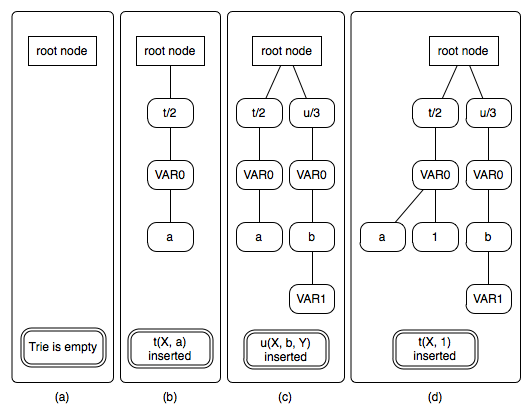
\includegraphics[scale=0.6]{tries.png}
    \caption{Using tries to represent terms.}
    \label{fig:tries_use}
  \end{figure}
  
  The Figure \ref{fig:tries_use} shows a trie with three terms. First, in \textbf{(a)} the trie is represented by a \textit{root node} and has
  no terms. Next, in \textbf{(b)} the term \textbf{t(X, a)} is inserted and three nodes are created that represent each part of the term.
  In \textbf{(c)} a new term, \textbf{u(X, b, Y)} is inserted. This new term differs from the first one and a new distinct branch is created.
  Finally, in \textbf{(d)}, the input term is \textbf{t(Y, 1)} and only a new node needs to be created as this term shares two nodes
  with \textbf{t(X, a)}.
  
  Yap and XSB use two levels of tries to implement tabling:
  
  \begin{itemize}
    \item One level stores subgoal calls for each predicate;
    \item The second level stores answers for a specific subgoal.
  \end{itemize}
  
  \begin{figure}[ht]
     \centering
       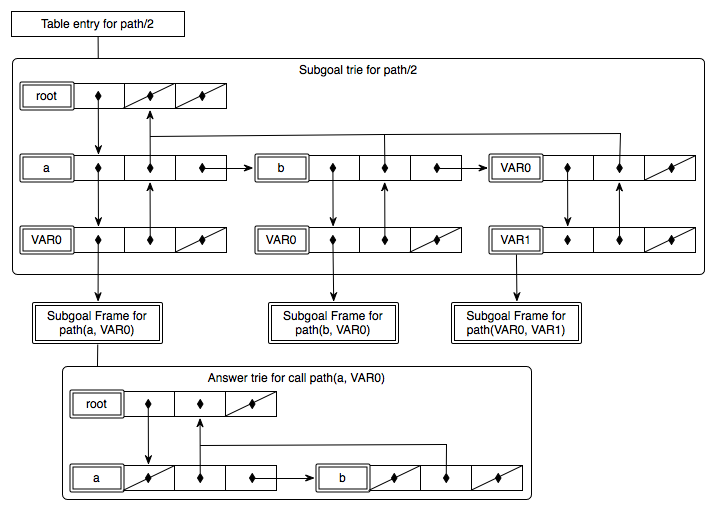
\includegraphics[scale=0.6]{two_level_tries.png}
     \caption{Organizing the table space with tries.}
     \label{fig:table_space_tries}
   \end{figure}
  
  For both levels, each trie node usually contains four fields. The first field represents the \textbf{symbol} (or \textbf{atom})
  of the transition. The second points to the first descendant transition (called the \textbf{child node})
  and the third stores a pointer to the \textbf{parent} node.
  The fourth field points to a \textbf{sibling} node.
  
  When the chain of sibling nodes gets too big, an hashing scheme is dynamically employed to provide direct
  access to nodes, optimizing the search of transitions.
  
  Each tabled predicate contains a \textit{table entry} that points to a \textit{subgoal trie}.
  Only the subgoal arguments are stored.
  Each different call to a tabled predicate corresponds to a unique path through the trie.
  The leaf points to a data structure called \textit{subgoal frame}. The frame stores
  information about the subgoal, namely an entry point to its \textit{answer trie}.
  
  The answer trie stores answers to the subgoal. When inserting answers only substitutions
  for the variables in the call are stored. This optimization is called \textit{substitution factoring} \cite{RamakrishnanIV-95}.
  
  Figure \ref{fig:table_space_tries} shows the table space after evaluating \textbf{path(X, Z)} (example in Figure \ref{fig:tabling_path}).
  Subgoals \textbf{path(X, Z)}, \textbf{path(b, Z)} and \textbf{path(a, Z)} are stored in the \textbf{path/2} subgoal trie.
  Only the answer trie for \textbf{path(a, Z)} is represented. Using substitution factoring only \textbf{Z = b} and \textbf{Z = a}
  were stored.
  
  \subsubsection{Subgoal frames}
  
  A subgoal frame contains general information about the state of a tabled subgoal.
  To access answers, this frames contain a pointer to the root of the answer trie.
  
  A chain of answers used by consumers is also kept in the form of head and tail pointers.
  In XSB, a \textit{answer return list} is built and the consumer has a pointer to the last consumed node of the list.
  In Yap, answers are chained using the \textbf{child} pointer of the leaf answer nodes. Yap's consumers only keep
  the last consumed answer leaf. The last consumed answer pointer is an \textit{answer continuation}. Thus, when
  a consumer needs to verify or consume the next available answer, it uses the continuation to retrieve the next
  answer, following the chain of answers. To load an answer, the trie nodes are traversed in bottom-up order and the answer is reconstructed.
  
  To facilitate memory management, both systems link subgoal frames by storing \textbf{next} and \textbf{previous} pointers in each subgoal frame,
  forming a double linked list.
  
  Information about the current evaluation state of the subgoal is usually kept. Yap has the following states:
  \textit{ready}, \textit{evaluating}, \textit{complete} and \textit{incomplete}.
  
  \subsubsection{Choice Point and Execution}
  
  The YapTab design mostly follows XSB's SLG-WAM approach (\cite{Sagonas-96} and \cite{Sagonas-98}).
  Both introduce the table space,
  a new set of registers, the \textit{freeze registers}, one per stack (local stack, heap and trail);
  an extension of the standard trail,
  called the \textit{forward trail}; and the tabling operations: \textit{tabled subgoal call},
  \textit{new answer}, \textit{answer resolution}, and \textit{completion}.
  
  The set of freeze registers says where stacks are frozen and protect the space belonging to suspended
  computations until the completion of the appropriate SCC takes place. They need to be adjusted
  in two different situations: when a computation suspends, increasing the portion of frozen stacks; and when a completion takes place,
  releasing part of space previously frozen.
  
  The forward trail is used to restore all the variable bindings to their state at the time the computation was suspended.
  Thus, the WAM trail is extended with parent trail entry pointers to create this new trail.
  Also, a new register is created, the \textbf{TR\_FZ} trail freeze register.
  
  The differences between SLG-WAM and YapTab reside in the data structures and algorithms used to control the process of leader detection
  and the scheduling of unconsumed answers. Each engine is described in the next two sections.
  
  \subsubsection{SLG-WAM}
  
  The SLG-WAM considers that evaluation control should be done at the level of the data structures
  corresponding to first calls to tabled subgoals, and does so by associating \textit{completion frames}
  to generator nodes \cite{Sagonas-98}.
  
  The \textit{completion stack} maintains, for each subgoal $S$, a representation of the deepest subgoal
  $S_{dep}$ upon which $S$ or any subgoal on top of $S$ may depend.
  
  When $S$ and all subgoals on top of $S$ have exhausted all program and answer clause resolution,
  $S$ is checked for completion. If $S$ depends on no subgoals deeper than itself, $S$ and
  all subgoals on top of $S$ are completely evaluated. Otherwise, if $S_{dep}$ is deepr in the completion
  stack than $S$, $S$ may depend upon subgoals that appear below it in the completion stack, and cannot be completed \cite{Sagonas-98}.
  
  A one-to-one correspondence exist between completion stack frames and generator nodes, as the completion stack frame
  is pushed onto the stack when a new tabled subgoal is called. A completion frame is popped off when a subgoal is
  completed. Also, each subgoal frame contains a pointer to completion frame.
  
  Consumer and generator choice points are extended to support the suspend and resume mechanism.
  
  The generator choice contains the following extra data: an explicit pointer of the failure continuation to take
  upon backtracking out of the choice point; a cell that records the value of a new global register,
  called the \textbf{RS} (\textit{root subgoal register}) register,
  which points to the root subgoal of the node currently under execution;
  a pointer to the subgoal frame; a set of freeze registers, so that the stored values can be restored later on;
  and an area called the \textit{substitution factor}, the set of free variables which exist in the terms in the argument registers.
  
  The consumer choice point is extended with: a copy of the \textbf{RS} register; a pointer of the failure continuation to take
  upon backtracking; a substitution factor; the last consumed answer continuation; and a pointer to chain
  together all consumer choice points of the same subgoal. 

  \subsubsection{YapTab}
  
  In YapTab, it is considered that the control of leader detection and scheduling of unconsumed answers should be
  performed through the data structures corresponding to repeated calls to tabled subgoals, and it associates a new
  data structure, the \textit{dependency frame}, to consumer nodes \cite{Rocha-00a}.
  
  Dependency frames are used to check for completion points and to move across the consumer nodes with unconsumed answers,
  thus they are linked together, forming the \textit{dependency space}.
  They reduce the number of extra fields in tabled choice points.
  
  Each consumer choice point contains a field that points to the respective dependency frame. Generator choice points
  have two extra fields: a pointer to the subgoal frame; the substitution factor; and, optionally, a pointer to a dependency frame. This pointer
  is only used when local scheduling is employed. A generator node for local scheduling only exports its answers to the calling
  environment when all clauses for the subgoal have been exhausted, hence it must act like a consumer.
  
  In SLG-WAM if we want to release space previously frozen, the stored values in the generator choice point are used. In
  YapTab, as they are not saved there, the top stack values kept in the youngest consumer choice point younger than
  the current completion point are used.
  
  Each dependency frame contains the following fields: the last answer continuation for this consumer called \textbf{try\_answer};
  a pointer to the consumer choice point (\textbf{cons\_cp}); the \textbf{leader} field which points to the leader node
  at creation time; and the \textbf{back\_leader} field that changes during evaluation, pointing to the leader node where we
  performed the last unsuccessful completion operation. 
  A new global register, called \textbf{TOP\_DF}, always points to the youngest dependency frame.
  
\section{Tabling by Call Subsumption} \label{sec:subsumption}

Although variant based tabling has proven to be greatly beneficial in solving some shortcomings of the SLD resolution,
other approaches are possible. Tabling by call subsumption aims to reuse answer computations by sharing answers from
\textit{more general} goals \cite{Johnson-99}.

When a subgoal is first called, a variant engine will lookup in the table space for a variant subgoal, one that is
identical by renaming the variables. If a subgoal already exists on the subgoal trie, a new consumer is created which
consumes answers from the variant subgoal.

Although a variant check is a light-weight operation computationally,
tabling engines using such checks can end up computing answers through program clause resolution, which takes time and space,
when they could retrieve answers from a subgoal that \textit{subsumes} the new call. By other words, a more specific subgoal
could consume answers from a general subgoal, which contains the full set of answers for the specific subgoal among the complete set.

Formally, if two subgoals $G$ and $G'$ exist, such that $S$ and $S'$ are the respective answer sets and
$G'$ subsumes $G$, we can conclude that $S \subseteq S'$.

The effects of using subsumptive checks are greater reuse of computed answers and reduced program clause resolution, yielding
superior time performance. In terms of space, improvements can be made since fewer calls and their associated answer sets
need to be preserved \cite{Johnson-99}.
However, implementing call subsumption poses various challenges:

\begin{itemize}
  \item Efficiently check for subsuming subgoals in the subgoal trie;
  \item The design of new mechanisms that represent answers and support fast retrieving of subsets that are only related to a subsumed call;
  \item Support for incremental retrieving of the answer subset. During evaluation is not possible for a subgoal to
  contain all answers, as the process of generating answers is incremental.
\end{itemize}

For illustration purposes, we describe the evaluation of \textbf{?- path(X, Z)} (Figure \ref{fig:tabling_path_sub}) using the program presented in Listing \ref{prolog_path}
and compare it against the variant approach in Figure \ref{fig:tabling_path}.

\begin{figure}[ht]
  \centering
    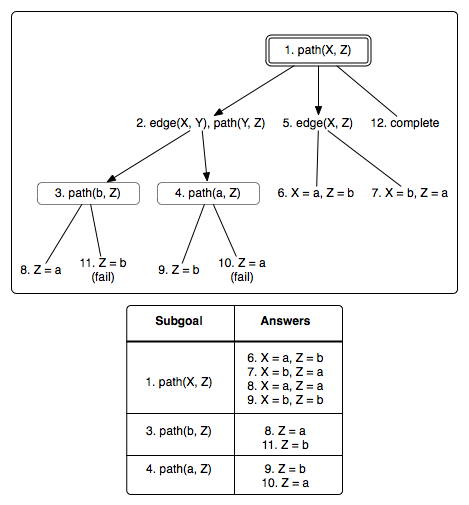
\includegraphics[scale=0.6]{tabling_path_sub.png}
  \caption{Tabling \textbf{path(X, Z)} using call by subsumption.}
  \label{fig:tabling_path_sub}
\end{figure}

At step 1 the subgoal \textbf{path(X, Z)} is called and a new generator node is created as there is no existing subgoals in the table space
that could be variant or subsuming. Being a generator node, it is evaluated using the program clauses (step 2). The first solution
for the \textbf{edge(X, Y)} predicate is evaluated using Prolog's standard rules and yields a subgoal call to \textbf{path(b, Z)} (step 3).

In variant tabling the engine would search for a variant subgoal in the table space, thus failing and creating a new generator node,
meanwhile expanding the execution tree by means of program clause resolution. In subsumptive tabling, the engine searches for a subsuming call,
and finds \textbf{path(X, Z)}. This subgoal
is more general than \textbf{path(b, Z)} and contains all the answers need for the subsumed goal.
A special type of consumer called a \textit{subsumptive consumer} is created. This consumer knows the subsuming subgoal and can retrieve
the answers that unify with the subsumed call.

As \textbf{path(X, Z)} has no answers and thus, no answers that can be consumed by \textbf{path(b, Z)}, the consumer node is suspended
and execution backtracks to node 2. The second clause of \textbf{edge/2} is tried and a new tabled subgoal is called: \textbf{path(a, Z)} (step 4).
Like \textbf{path(b, Z)}, this subgoal is subsumed by \textbf{path(X, Z)}, hence a new subsumptive consumer node is created. Execution suspends
once again because no answers are available and the engine goes back to node 1 to try the second \textbf{path/2} clause (step 5).

Solutions for \textbf{path(X, Z)} are found in steps 6 and 7, \textbf{X = a, Z = b} and \textbf{X = b, Z = a}, and stored in the answer set
for this generator node. Execution thus backtracks to node 1 and completion is attempted. Node 1 verifies that node 3 and 4 have
unconsumed answers and starts by resuming computation at node 3.

Node 3 being a subsumptive consumer looks up in the \textbf{path(X, Z)}
answer set for answers specific to \textbf{path(b, Z)}, finding one: \textbf{Z = a} (step 8). At this point, the consumer stores the answer
for later retrieval, so that answers can be immediately consumed when a variant subgoal is called.
Like variant tabling, the consumer keeps a last consumed answer continuation to know which answers have already been consumed.
Once the answer is stored, the variable bindings are propagated and a new answer to \textbf{path(X, Z)} is found: \textbf{X = a, Z = a}.
Node 3 tries to consume a new answer, but no new answers are available for this subgoal.

Execution suspends node 3 and resumes computation at node 4. Here \textbf{path(a, Z)} begins to consume answers from \textbf{path(X, Z)}
using the subsumption mechanism. The first answer in \textbf{path(X, Z)}, \textbf{X = a, Z = b}, unifies with the subsumed goal and
is consumed (step 9). By variable propagation, a new answer for \textbf{path(X, Z)} is also generated, \textbf{X = b, Z = b}.
Node 3 then tries to consume a new answer and finds \textbf{X = a, Z = a} (step 10). This new answer
is added to the \textbf{path(a, Z)} table space. As the new variable bindings are propagated, a new answer is also generated
for top subgoal, but the answer is repeated (\textbf{X = b, Z = a}), hence is not inserted into the table space.

As each consumer uses the available answers, execution backtracks to the leader node, \textbf{path(X, Z)}, that will once
again attempt completion. By using the last consumed answer continuation, it is verified that node 3 has unconsumed answers.
Execution thus resumes at node 3.

Node 3 inspects \textbf{path(X, Z)} answer set and consumes the next matching answer, \textbf{X = b, Z = b} (step 11). A new answer
for \textbf{path(b, Z)} is generated and variable bindings are propagated to the leader node. The new answer is already
stored in the table space and it is not used.

Once again, evaluation returns to the leader node and completion is attained (step 12) as each consumer has exhausted the
available answers.

This evaluation example, when compared to variant tabling, shows a smaller execution tree with less
program clauses expanded. The subsumptive computation also took less steps to complete and a greater
reuse of answers was done between \textbf{path(X, Z)}, \textbf{path(b, Z)} and \textbf{path(a, Z)}.

Although this example shows a very good performance of this method of evaluation, if we tried
to evaluate \textbf{path(a, Z)} and then \textbf{path(X, Z)}, no reuse could be done with \textbf{path(a, Z)}
because not previous subsuming goal was present. The more general subgoals are called first, the greater
the reuse in call subsumption.

Like variant tabling, the same four main operations are used when evaluating subsumptive subgoals.
These operations are very similar, with a few differences. Operations \textit{new answer} and
\textit{completion} remain the same, while the \textit{tabled subgoal call} and \textit{answer resolution}
work differently:

\begin{itemize}
  \item The \textit{tabled subgoal call} operation represents a call to a tabled subgoal.
  If the subgoal $c$ is called, a search for a subsuming subgoal $c'$ is done. If such subgoal is found,
  the new subgoal will be resolved using \textit{answer clause resolution}, thus consuming answers from the subgoal $c'$.
  If no subgoal $c'$ is found, then $c$ is inserted into the table space and the new generator node is evaluated using
  program clause resolution.
  
  \item The \textit{answer resolution} operation checks wether new answers from the table space are available for consumption.
  Each subsumptive consumer node uses an answer continuation that represents
  the set of remaining answers to be consumed. Given an answer continuation we inspect the answer trie from the subsuming subgoal
  and retrieve the next answer $T$ that matches with the subsumed goal. Once the answer is retrieved and loaded, the answer
  continuation is updated to reflect the new answer consumed.
\end{itemize}

The next sections describe two known techniques that implement subsumptive tabling. These two approaches were all implemented in XSB.

  \subsection{Dynamic Threaded Sequential Automata}\label{sec:dtsa}

  \textit{Dynamic Threaded Sequential Automata} (DTSA) is a data structure that provides good indexing and incremental
  returning of a subset of answers from a subsuming call to a subsumed call \cite{Rao-96}.
  
  This structure orders answers as they are generated, hence it can easily mark which answers were already retrieved, enabling
  efficient retrieval of the remaining answers.
  
  A DTSA is based on a \textit{Sequential Factoring Automaton} (SFA) but has a few more features for dealing with fast indexing
  and incremental retrieving of answers. SFA were introduced by S. Dawson et all in \cite{Dawnson-95}. 
  
  \subsubsection{Sequential Factoring Automaton: Basic search}
  
  A SFA solves the problem of retrieving an ordered subset of answers, starting from the oldest to the newest answer. It is an ordered
  tree-structure automaton and is very similar to a trie. It starts with a root as the start state and has edges as transitions
  that represent unifications. Every leaf represents a distinct term and the transitions on the path from the root to a leaf
  represent the operations necessary to unify the goal with the term at the leaf.
  
  Apart from ordering, SFAs differ from tries in that transitions from a state may not be unique and each transition in a trie
  denotes match operations, not unify operations.
  
  \begin{figure}[ht]
    \centering
      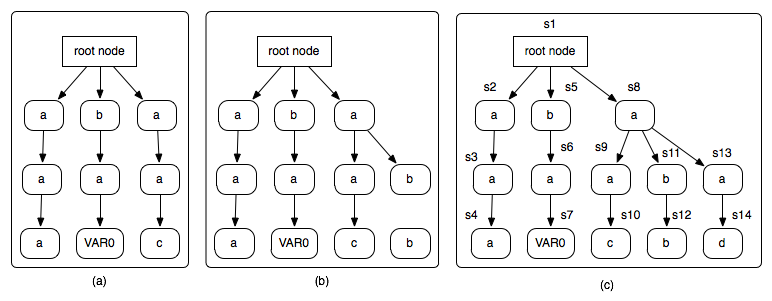
\includegraphics[scale=0.6]{sfa.png}
    \caption{Inserting answer terms in a SFA.}
    \label{fig:sfa_example}
  \end{figure}
  
  To insert a new term into a SFA, we must start by inserting symbols from the answer term into the root state.
  In each state we verify if the last transition $s$ matches the current term symbol $t$. If $t$ matches $s$
  we take the transition and advance to the next state; if not, a new transition for $t$ is created and we advance
  to the newly created state. When all term symbols $t$ are exhausted, the current state is marked as a leaf,
  representing a new answer.
  
  Figure \ref{fig:sfa_example} represents a SFA for the subgoal \textbf{p(X, Y, Z)} and
  illustrates a few phases in the lifetime of a SFA:
  
  \begin{enumerate}[(a)]
    \item Answers \textbf{p(a, a, a)}, \textbf{p(b, a, W)} and \textbf{p(a, a, c)} are currently stored.
    \item Answer \textbf{p(a, b, b)} is inserted.
    \item New answer: \textbf{p(a, a, d)}.
  \end{enumerate}
  
  When a new subgoal $G$ subsumed by the subgoal $G'$ is first called, we must determine the assignments
  from $G'$ to the sub-terms of $G$, because only variable substitutions are inserted into a SFA.
  The assignments are usually stored under the choice point.
  
  For example, if $G'$ is \textbf{p(X, Y, Z)} and $G$ is \textbf{p(a, a, V)}, the variable assignments
  are $X = a, Y = a, Z = VAR0$. During unification operations, we must unify the first SFA symbol
  to $a$, then to $a$ again, and finally with $VAR0$.
  Once a variable is \textit{bound}, subsequent unify operations must unify with the bounded sub-term.
  
  The unification process starts in the root state with an empty \textit{continuation stack}.
  When a state $s$ is reached, the leftmost transition that unifies with the current $G$ assignment is chosen,
  this is called the \textit{applicable transition}.
  Before moving to the next state, we select the next applicable transition and push it on the continuation stack.
  If no applicable transitions are available at state $s$ or if an answer was found, we pop a transition from
  the stack and use it to search for more answers. Once no more transitions can be taken and the stack is empty, the
  search process ends.
  
  Using the SFA in Figure \ref{fig:sfa_example} and the subgoal $G$, \textbf{p(a, a, V)}, the search mechanism starts
  at the root state and is ready to retrieve all answers that unify with $G$.
  The first applicable transition is $s1 \rightarrow s2$ because it unifies with the first symbol: $a$. The transition
  $s1 \rightarrow s5$ can not be pushed into the continuation stack because it does not unify, but $s1 \rightarrow s8$ does.
  In state $s2$ only one transition is available, thus nothing is pushed into the stack.
  Transition $s2 \rightarrow s3$ unifies with symbol $a$ and we move to state $s3$. Here, the variable $VAR0$ (that represents $V$)
  can unify with $a$, thus we can get to state $s4$, arriving at a leaf state and a new answer, \textbf{V = a}.
  
  Next, the process must use the continuation stack to retrieve more answers. Transition $s1 \rightarrow s8$ is popped from the stack
  and we arrive at state $s8$ with 3 available transitions. Using the previous rules, a new answer is retrieved,
  \textbf{V = c} and the continuation stack contains the transition $s8 \rightarrow s13$.
  
  Finally, once states $s8$, $s11$ and $s14$ are visited, the process arrives at a leaf state and a new answer, \textbf{V = d}, is retrieved.
  The process finishes and every answer that is specific to \textbf{p(a, a, V)} is found.
  
  \subsubsection{Threaded Sequential Automata: Indexing}
  
  A \textit{Threaded Sequential Automata} extends the SFA with a concept called
  \textit{equivalent states}. One state $s1$ is equivalent to state $s2$ if when $s1$ is taken, $s2$ is also
  guaranteed to be visited. For example, in Figure \ref{fig:sfa_example}, whenever states $s2$ and $s8$ are
  visited, states $s8$ and $s9$ are also guaranteed to be visited, as they denote the same path.
  
  A SFA is converted to a TSA by adding \textit{equivalence links} between equivalent states.
  The SFA in Figure \ref{fig:sfa_example} was transformed into a TSA in Figure \ref{fig:tsa_example}.
  
  \begin{figure}[ht]
    \centering
      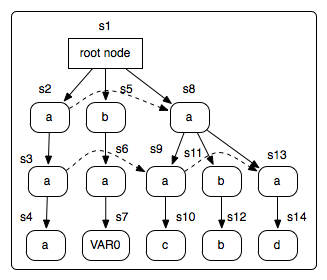
\includegraphics[scale=0.6]{tsa.png}
    \caption{SFA transformed into a TSA}
    \label{fig:tsa_example}
  \end{figure}
  
  In the TSA, the concept of applicable transitions is changed. Now it is also possible to push equivalence links
  into the continuation stack as if they were normal transitions. So, if we were at state $s3$ we use
  the transition to $s9$ and then to $s13$ instead of going from the start state.
  
  Although equivalence links provide an efficient indexing mechanism, they must be used with care. If not,
  some situations arise where following equivalence links lead to repeated answers and answers in the incorrect order \cite{Rao-96}.
  The selection of transitions must consider only \textit{safe transitions}, which reach answers that cannot be reached through the pending
  transitions on the stack.
  So, if the process is at state $s2$ and the transition $s1$ to $s8$ is already on the
  stack, we can not use the equivalence link $s2$ to $s8$, as the transition $s1$ to $s8$ already covers the same branch.
  
  If we followed only safe transitions, no equivalence links would be used, hence we must check if there is any
  equivalence link that can be used in the next state that covers the same answers if we pushed the
  usual next applicable transition into the stack. Thus, at state $s2$ we would use the equivalence $s2$ to $s8$, instead of
  the transition $s1 \rightarrow s8$.
  
  \begin{figure}[ht]
    \centering
      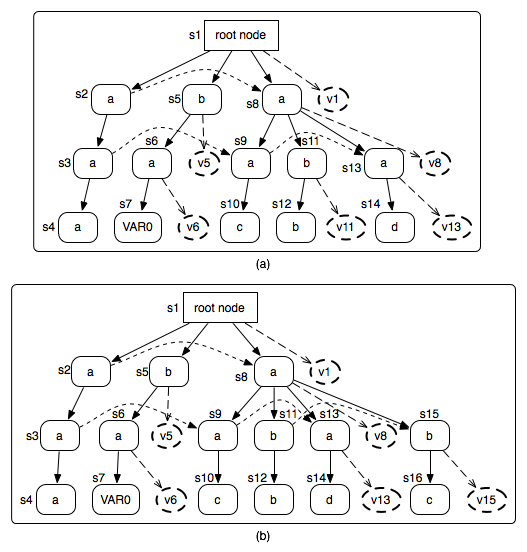
\includegraphics[scale=0.6]{dtsa.png}
    \caption{DTSA before and after inserting answer \textbf{p(a, b, c)}}
    \label{fig:dtsa_example}
  \end{figure}
   
  \subsubsection{Dynamic Threaded Sequential Automata: Incremental answer retrieval}
  
  The previously described mechanisms only work if we have the complete set of answers for the subsuming subgoal.
  A new mechanism that deals with incomplete answer sets must be devised, so that after all current answers
  are retrieved, the continuation stack can be used to retrieve newly inserted answers.
  
  The Dynamic Threaded Sequential Automata extends the TSA with special transitions in states
  were new transitions can be inserted or in states were no equivalence links exist.
  Figure \ref{fig:dtsa_example} illustrates two DTSAs: (a) shows the converted TSA from Figure \ref{fig:tsa_example}, and
  (b) the resulting DTSA after inserting the answer \textbf{p(a, b, c)}.
  
  During answer retrieval, if no answer is found and the top of the continuation stack contains
  a transition to a special state, the process stops and the continuation stack is saved along the last state
  visited.
  Later on, when new answers must be retrieved, the last state is used to transform the stack to account for new states that
  were introduced during the insertion of new terms. If the new stack contains a valid transition, it
  can now be used as usual.
  
  For example, retrieving answers to subgoal \textbf{p(a, X, c)} from the DTSA (a) in Figure
  \ref{fig:dtsa_example} results in the answer \textbf{p(a, a, c)} and a continuation formed by the last
  visited state $s13$ and the stack containing (from bottom to top): $[s1 \rightarrow v1, s8 \rightarrow v8, s13 \rightarrow v13]$.
  After the new answer \textbf{p(a, b, c)} is inserted into the DTSA in Figure \ref{fig:dtsa_example} and
  a consumer is resumed to consume new answers, it checks if new answers are available and the continuation stack
  is thus transformed by using the last visited state $s13$ into: $[s1 \rightarrow v1, s8 \rightarrow s15]$. Now
  the answer \textbf{p(a, b, c)} can be easily retrieved using the transition $s8 \rightarrow s15$.
  
  \subsubsection{Table Space}
  
  This new DTSA mechanism was implemented in XSB by extending the variant engine \cite{Rao-96}.
  
  First, each subgoal frame for generator nodes now contains both an answer trie and a DTSA.
  Answer tries are used to check for duplicate answers and the DTSA is created lazily, when a new subsumed node
  first appears.
  
  Each subsumed subgoal in the call trie keeps an answer return list that is built using the DTSA technique.
  This answer list is used when variant goals of the subsumed goal are called, thus instead of using
  the DTSA, answers are retrieved directly by traversing the linked list.
  
  When a subgoal is marked as complete, its answer trie is compiled into WAM instructions and the DTSA is deleted.
  Answers for subsumed goals are then retrieved by using trie instructions through the usual WAM backtracking
  mechanism.
  
\subsection{Time Stamped Tries} \label{sec:time_stamped_tries}

  \textit{Time Stamped Tries} (TST) is another mechanism that was implemented in XSB
  to support tabling by call subsumption \cite{Johnson-99}.
  
  TST is a relatively simple technique based around the idea of augmenting a trie with information about the relative time
  its terms were inserted. The time of insertion of each term is called its time stamp and is represented by a
  positive integer. The time stamps are then used for incremental answer retrieval.
  
  \begin{figure}[ht]
    \centering
      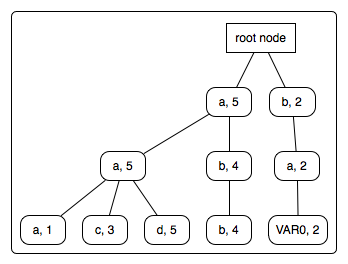
\includegraphics[scale=0.6]{tst_1.png}
    \caption{Time Stamped Trie for subgoal \textbf{p(X, Y, Z)}.}
    \label{fig:tst_1}
  \end{figure}
  
  For each node in a trie, we extend it by including a time stamp. Along the augmented trie, the maximum time stamp
  $T$ is also stored, thus allowing the insert mechanism to know the next time stamp to use for new trie paths.
  An example TST for the subgoal \textbf{p(X, Y, Z)} is represented in Figure \ref{fig:tst_1}.
  By looking at the leaf nodes, the order of answer insertion
  can be readily known: \textbf{p(a, a, a)}, \textbf{p(b, a, VAR0)}, \textbf{p(a, a, c)}, \textbf{p(a, b, b)} and then
  \textbf{p(a, a, d)}.
  
  \subsubsection{New answers}
  
  The process of inserting a new answer into a TST starts by traversing matching nodes as long the stored symbols
  match the new answer. If the current symbol does not match, the process changes from search to insert mode and
  new nodes are inserted to represent a new trie path. Once the leaf node is created, each node from leaf to root
  is traversed and its time stamp is updated to $T + 1$.
  
  \begin{figure}[ht]
    \centering
      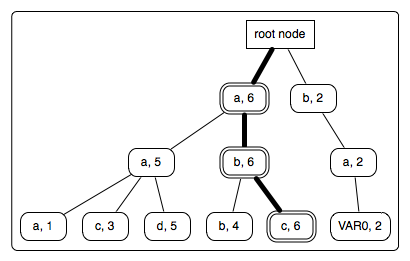
\includegraphics[scale=0.6]{tst_2.png}
    \caption{Time Stamped Trie from Figure \ref{fig:tst_1} after inserting the answer \textbf{p(a, b, c)}.}
    \label{fig:tst_2}
  \end{figure}
  
  Figure \ref{fig:tst_2} shows the TST from Figure \ref{fig:tst_1} after a new answer \textbf{p(a, b, c)} was inserted.
  Note that each node from the answer leaf node to root node was updated with the new timestamp (6). Apart from
  the time stamps, search and insertion in TSTs work exactly the same as tries.
  
  \subsubsection{Retrieving answers}
  
  Retrieving all answers that are specific to a subsumed subgoal $G$ from a TST with answers from subgoal $G'$
  works by navigating the TST and unifying the variable values that are assigned from $G'$ to $G$.
  If we wanted to retrieve answers to the subgoal \textbf{p(a, a, X)} from the TST in Figure \ref{fig:tst_2},
  during the subgoal call we determine the assignments relatively to \textbf{path(X, Y, Z)}: $X = a, Y = a, Z = VAR0$,
  and store them under the choice point. Then, these values $[a, a, VAR0]$ are then unified
  with the trie symbols, thus finding answers that are specific to $G$.
  
  Like tries, TSTs only store substitutions for variables, thus we must unify
  the first sub-term $a$, then $a$ again and then the variable, which unifies with any symbol.
  During the unification process, if a variable appears multiple times, it must unify with
  any previous sub-term assignment.
  
  Time stamps guide the answer unification process by filtering transitions to already explored branches, where
  answers were already retrieved, thus avoiding repeated answers.
  
  The unification process that finds new answers by using a time stamp is separated from the process
  of unifying the retrieved answers with the subsumed subgoal. This \textit{two-tier mechanism} is key to the space and time
  efficiency of the design of TSTs \cite{Johnson-99} and allows identification of all relevant answers that have
  been added since the last time a search operation was done by using the time stamp.
  
  \subsubsection{Table Space}

  The table space in this technique extends the variant table space by
  using TSTs instead of answer tries for subsuming goals.
   
  Each subsumed subgoal in a call trie stores the last search time stamp $t$. The process of
  incrementally searching for new answers in a TST will use $t$ and update it after the process completes.
  When a subsumptive subgoal is first called $t$ is set to $0$, thus initially allowing the retrieval of all
  relevant answers.
  
  The subgoal in the call trie also stores an answer return list. Each time new answers are identified, they are appended
  to this linked list. The original subsumptive consumer and its variant subgoals will then consume answers from it. If no
  new answers can be retrieved from the list, the TST process is employed to identify more answers from the subsuming TST,
  inserting them into the list.
  
  Each TST node maintains a time stamp index which stores all transitions in reverse order.
  It is not until a subsumed subgoal is first called that all time stamp related structures are created, thus
  allowing a more efficient use of space.
  
  Like DTSAs, the TST indexing mechanism is only used in incomplete subsuming calls, for complete calls
  the more specific goals all use compiled trie instructions, and unification is performed naturally at
  the WAM engine level.
  
  The biggest advantage of using TSTs instead of DTSA is in terms of space complexity. In TSTs, the maximum table space
  used is at most twice that of the variant engine. For DTSAs, the space used is at least double, but in the worst
  case can be quadratic. DTSA is at advantage in terms of speed, because it supports identification of answers and
  unification in one step, thus answers can share some elementary unifications. In TSTs, identifying answers
  and doing answer unification is a two step process, thus it takes more time to construct all answers. 

\subsection{Finding subsuming goals}

Both DTSA and TST use a similar method that given a call trie $C$ and a subgoal $G$
is able to find a subgoal $G'$ that subsumes $G$.

The search is performed by recursively backtracking through the call trie $C$, trying
to match the node symbols with sub-terms or symbols from $G$.

A non-variable symbol from $G$ must only match with an identical symbol from $C$ and
these types of unifications are always tried first.
If the current trie symbol is a variable, for example $X$, on the first occurrence $X$
is bound to the respective $G$ sub-term
and match succeeds; on the next occurrences of $X$, the current sub-term from $G$ must
be identical to the term bound to $X$. Through the backtracking process, bound variables are
always tried before unbound variables.

Favoring constant values before variables, results in a mechanism that finds \textit{minimally subsuming calls}.
Also, if there is some variant call $G''$ in $C$, $G''$ is found before any other subgoal. If no variant 
or no subsuming call are found, it is possible to save the trie node to insert a new variant call.
This trie node is where the first backtracking occurred or when the first occurrence of
an already seen $G$ variable that could not be paired to a bound trie variable, and instead
must be bound to an unbound trie variable for the process to continue.
The new variant path is then used to keep information about the subsumed goal state in
the leaf call trie node.


\chapter{Table Space and Subsumptive Tabling}

In this chapter, the table space organization for both variant and subsumption tabling engines are described.
First, the table space used to support call by variance for both SLG-WAM and YapTab is explained. Because
they share a lot of similarities, the description covers the common ground between the two systems.
Next, we explore two known mechanisms that
modify the previous table space for call by subsumption. Those two mechanisms have already been implemented in XSB
\cite{Rao-96, Johnson-99}.

\section{Table Space} \label{sec:table_space}

Implementing a tabling engine on a Prolog system involves the design of compact and time efficient data structures
to organize the table space. The table space is heavily used throughout the evaluation process in various operations:

\begin{itemize}
  \item to lookup if a subgoal is in the table, and if not insert it;
  \item to verify wether a newly found answer is already in the table, and if not insert it;
  \item to retrieve answers for consumer nodes.
\end{itemize}

\subsection{Tries}

Clearly, the success of tabling is highly dependent on the data structures used.
Both Yap \cite{Rocha-00a} and XSB \cite{RamakrishnanIV-95} use a trie-based tabling approach.

Tries were initially proposed to index dictionaries \cite{Fredkin-62} and have since been generalized to index recursive data structures
such as terms. The essential idea underlying a trie is to partition a set $T$ of terms based upon their structure,
hence common term prefixes are represented only once.

A trie is a tree-structured automaton with the root as the start state and each leaf state is associated with a term in $T$.
Each state specifies the position to be inspected in the input term on reaching that state.
The outgoing transitions specify the function symbols expected at that position.
A transition is taken if the current symbol in the input term matches the symbol of the transition.
If we recursively reach a leaf state we say that the input term \textit{matches} the term represented by the leaf state.
A complete path, from the root to a leaf, corresponds to a pre-order traversal of the matching term.
If no transition can be taken, the lookup operation fails. On the other hand, for an insert operation
we add a new outgoing transition for the current input symbol and a new node, which is linked to this transition.
To complete the insert operation, we consume the rest of the input term, until a leaf node is created that represents
the newly inserted term.

Given the nature of tries, the following conclusions can be made:

\begin{itemize}
  \item it is possible to do a single pass check/insert. If the lookup
  fails, it is possible to complete an insert operation using the last lookup state;
  \item the efficiency and memory consumption of a
  particular trie depends on the percentage of terms that have common prefixes.
\end{itemize}

When creating transitions for variables, we use the format outlined by Bachmair \textit{et al} \cite{Bachmair-93},
described in Section \ref{sec:variant_tabling}.

\begin{figure}[ht]
  \centering
    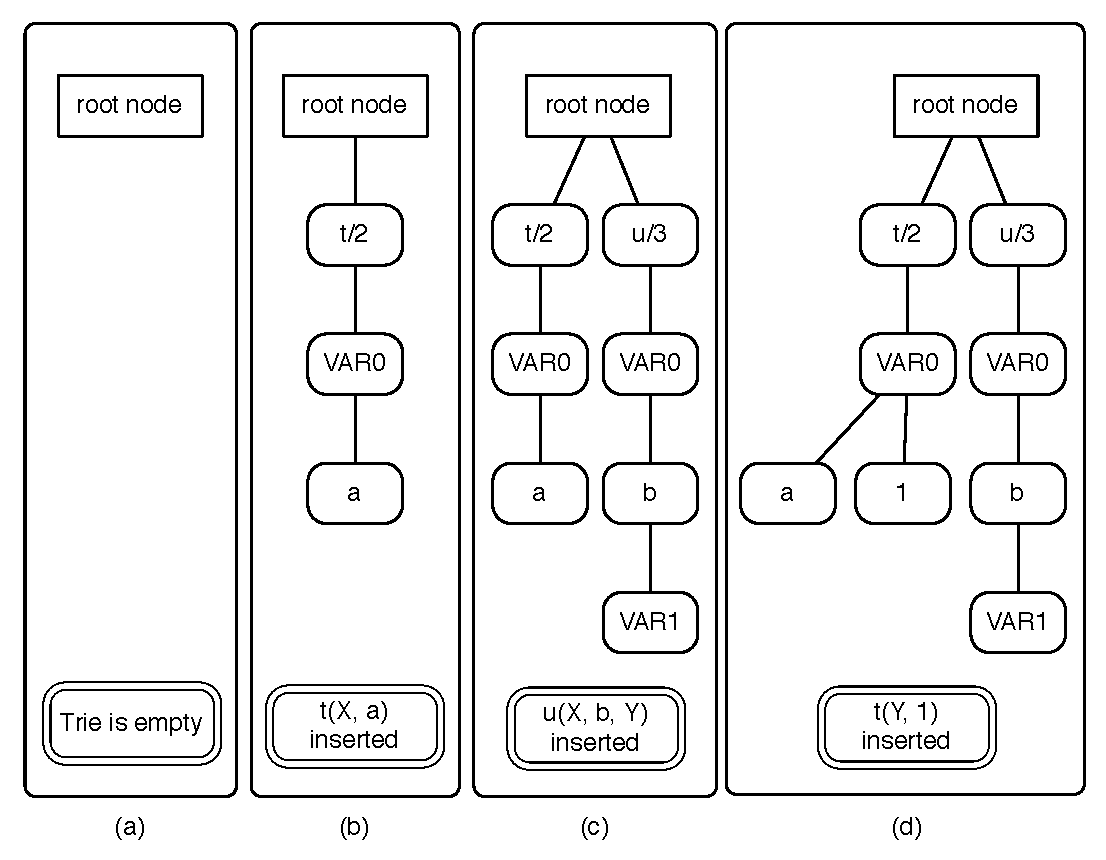
\includegraphics[scale=0.6]{tries.pdf}
  \caption{Using tries to represent terms.}
  \label{fig:tries_use}
\end{figure}

Figure \ref{fig:tries_use} shows a trie with three terms. First, in \textbf{(a)} the trie is represented by a \textit{root node} and has
no terms. Next, in \textbf{(b)} the term \texttt{t(X,a)} is inserted and three nodes are created that represent each part of the term.
In \textbf{(c)} a new term, \texttt{u(X,b,Y)} is inserted. This new term differs from the first one and a new distinct branch is created.
Finally, in \textbf{(d)}, the input term is \texttt{t(Y,1)} and only a new node needs to be created as this term shares two nodes
with \texttt{t(X,a)}.

Yap and XSB use two levels of tries to implement tabling:

\begin{itemize}
  \item One level stores subgoal calls for each predicate;
  \item The second level stores answers for a specific subgoal.
\end{itemize}

\begin{figure}[ht]
   \centering
     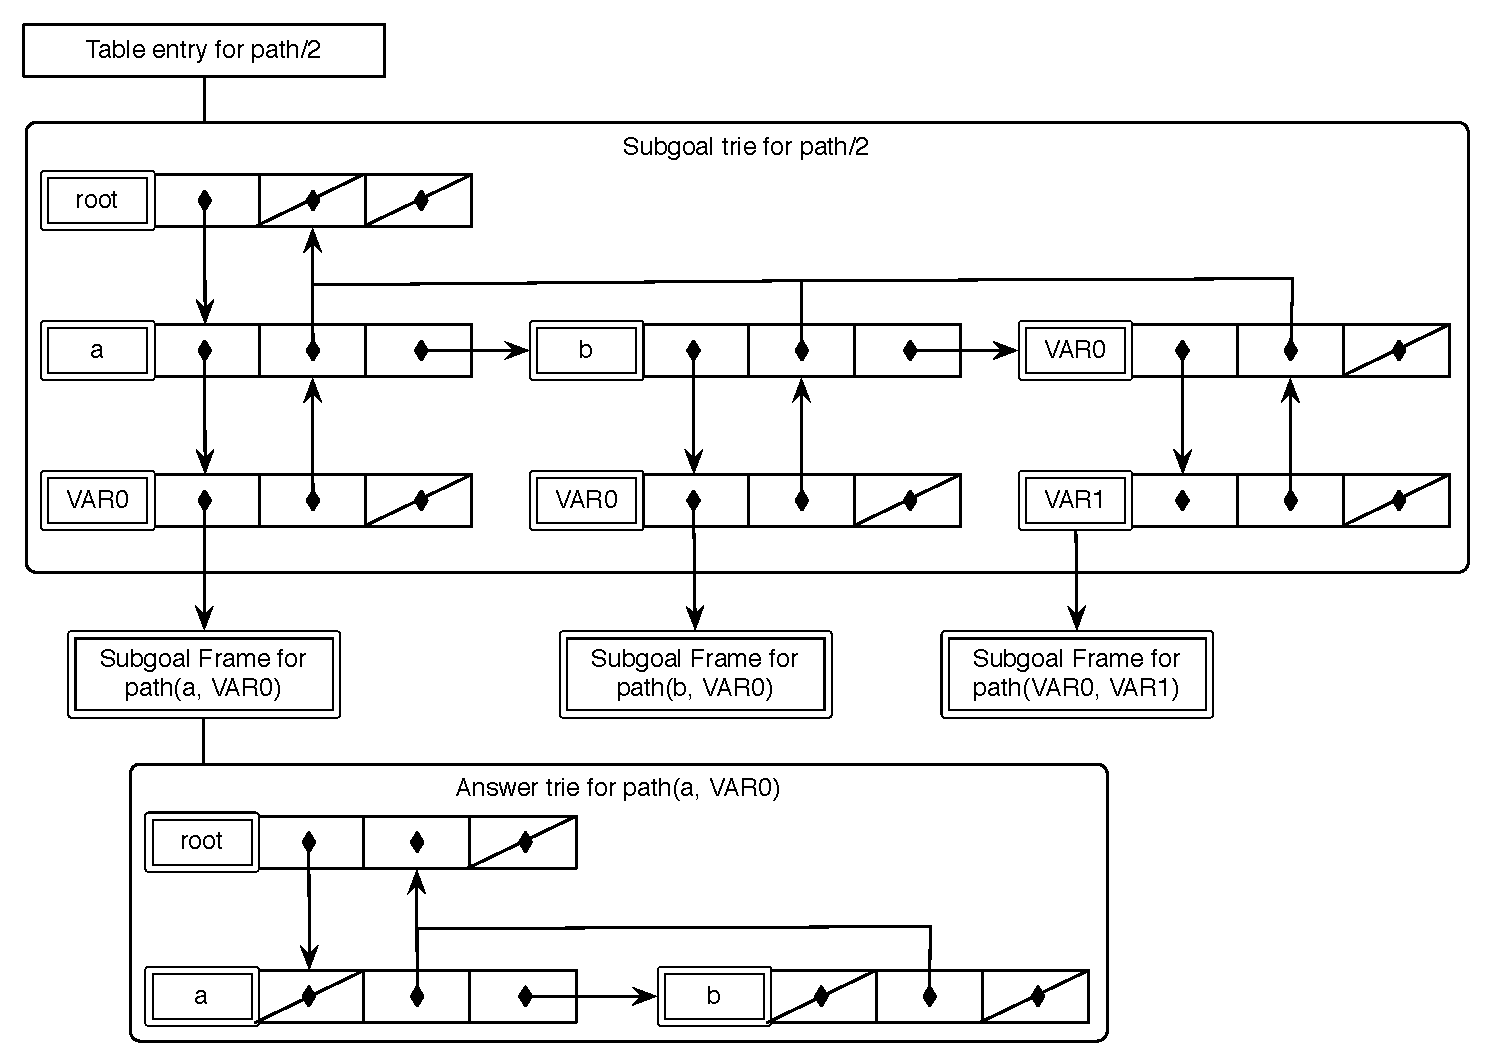
\includegraphics[scale=0.6]{two_level_tries.pdf}
   \caption{Organizing the table space with tries for variant tabling.}
   \label{fig:table_space_tries}
 \end{figure}

For both levels, each trie node usually contains four fields. The first field represents the \textbf{symbol} (or \textbf{atom})
of the transition. The second points to the first descendant transition (called the \textbf{child node})
and the third stores a pointer to the \textbf{parent} node.
The fourth field points to a \textbf{sibling} node.

When the chain of sibling nodes gets too big, an hashing scheme is dynamically employed to provide direct
access to nodes, optimizing the search of transitions.

Each tabled predicate contains a \textit{table entry} that points to a \textit{subgoal trie}.
Only the subgoal arguments are stored.
Each different call to a tabled predicate corresponds to a unique path through the trie.
The leaf points to a data structure called \textit{subgoal frame}. The frame stores
information about the subgoal, namely an entry point to its \textit{answer trie}.

The answer trie stores answers to the subgoal. When inserting answers only substitutions
for the variables in the call are stored. This optimization is called \textit{substitution factoring} \cite{RamakrishnanIV-95}.

Figure \ref{fig:table_space_tries} shows the table space after evaluating \texttt{path(X,Z)} (example in Figure \ref{fig:tabling_path}).
Subgoals \texttt{path(X,Z)}, \texttt{path(b,Z)} and \texttt{path(a,Z)} are stored in the \texttt{path/2} subgoal trie.
Only the answer trie for \texttt{path(a,Z)} is represented. Using substitution factoring only \texttt{Z = b} and \texttt{Z = a}
are stored.

\subsection{Subgoal Frames}

A subgoal frame contains general information about the state of a tabled subgoal.
To access answers, this frames contain a pointer to the root of the answer trie.

A chain of answers used by consumers is also kept in the form of head and tail pointers.
In XSB, a \textit{answer return list} is built and the consumer has a pointer to the last consumed node of the list.
In Yap, answers are chained using the \textbf{child} pointer of the leaf answer nodes. Yap's consumers only keep
the last consumed answer leaf. The last consumed answer pointer is an \textit{answer continuation}. Thus, when
a consumer needs to verify or consume the next available answer, it uses the continuation to retrieve the next
answer, following the chain of answers. To load an answer, the trie nodes are traversed in bottom-up order and the answer is reconstructed.

To facilitate memory management, both systems link subgoal frames by storing \textbf{next} and \textbf{previous} pointers in each subgoal frame,
forming a double linked list.

Information about the current evaluation state of the subgoal is usually kept. Yap has the following states:
\textit{ready}, \textit{evaluating}, \textit{complete} and \textit{incomplete}.

\section{Tabling by Call Subsumption} \label{sec:subsumption}

Although variant based tabling has proven to be greatly beneficial in solving some shortcomings of the SLD resolution,
other approaches are possible. Tabling by call subsumption aims to reuse answer computations by sharing answers from
\textit{more general} goals \cite{Johnson-99}.

When a subgoal is first called, a variant engine will lookup in the table space for a variant subgoal, one that is
identical by renaming the variables. If a subgoal already exists on the subgoal trie, a new consumer is created which
consumes answers from the variant subgoal.

Although a variant check is a light-weight operation computationally,
tabling engines using such checks can end up computing answers through program clause resolution, which takes time and space,
when they could retrieve answers from a subgoal that \textit{subsumes} the new call. By other words, a more specific subgoal
could consume answers from a general subgoal, which contains the full set of answers for the specific subgoal among the complete set.

Formally, if two subgoals $G$ and $G'$ exist, such that $S$ and $S'$ are the respective answer sets and
$G'$ subsumes $G$, we can conclude that $S \subseteq S'$.

The effects of using subsumptive checks are greater reuse of computed answers and reduced program clause resolution, yielding
superior time performance. In terms of space, improvements can be made since fewer calls and their associated answer sets
need to be preserved \cite{Johnson-99}.
However, implementing call subsumption poses various challenges:

\begin{enumerate}[(a)]
\item How to efficiently check for subsuming subgoals in the subgoal trie;
\item How to design new mechanisms to represent answers supporting fast retrieval of subsets that are only related to a subsumed call;
\item How to support incremental retrieving of the answer subset. Note that, during evaluation, it may be not possible for
the subsuming call to contain all answers, as the process of generating answers is incremental.
\end{enumerate}

For illustration purposes, in Figure \ref{fig:tabling_path_sub}, we describe the evaluation of \texttt{path(X,Z)}
using the program presented in Figure \ref{fig:prolog_path}
and compare it against the variant approach in Figure \ref{fig:tabling_path}.

\begin{figure}[ht]
\centering
  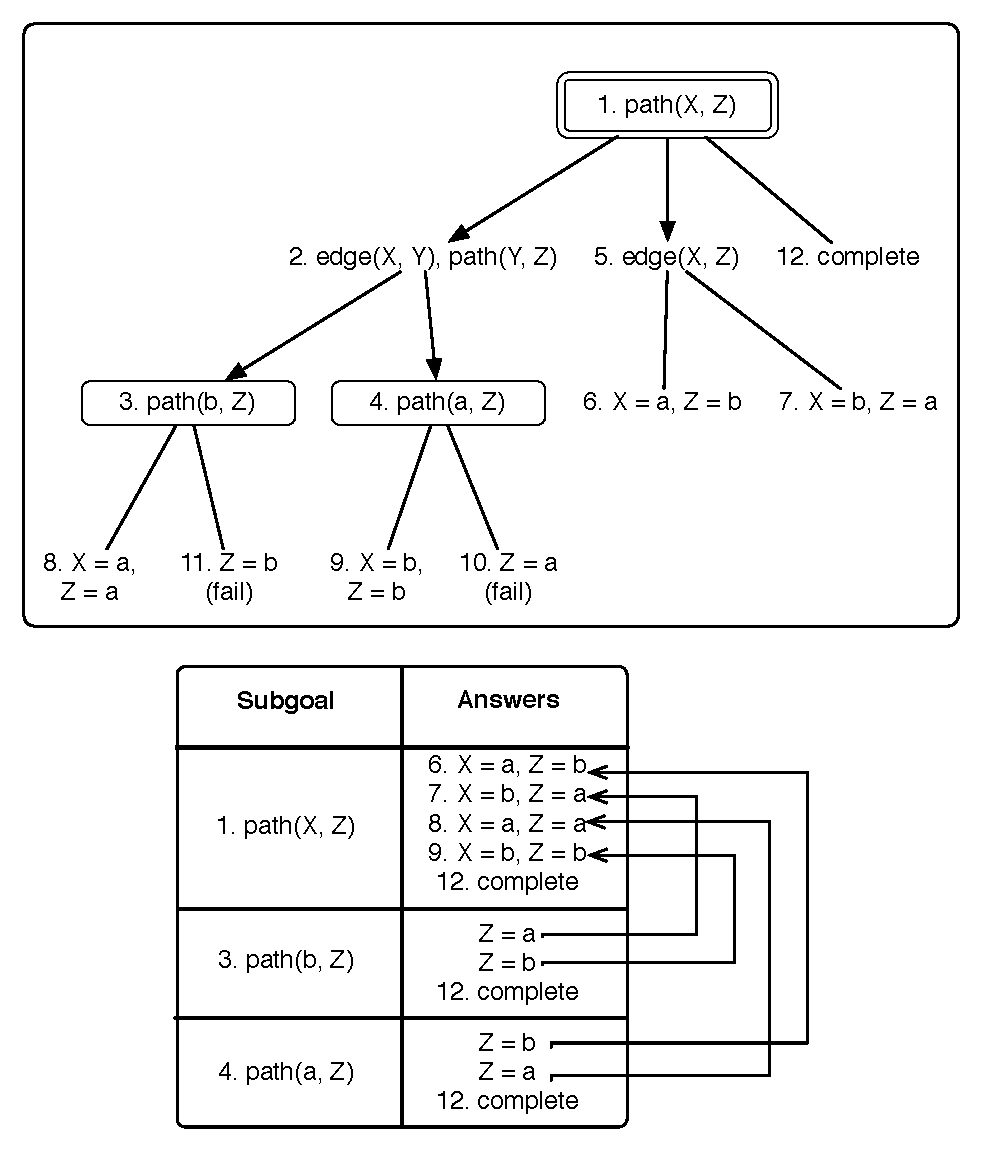
\includegraphics[scale=0.6]{tabling_path_sub.pdf}
\caption{Tabling \texttt{path(X,Z)} using call by subsumption.}
\label{fig:tabling_path_sub}
\end{figure}

At step 1 the subgoal \texttt{path(X,Z)} is called and a new generator node is created as there is no existing subgoals in the table space
that could be variant or subsuming. Being a generator node, it is evaluated using the program clauses (step 2). The first solution
for the \texttt{edge(X,Y)} predicate is evaluated using Prolog's standard rules and yields a subgoal call to \texttt{path(b,Z)} (step 3).

In variant tabling the engine would search for a variant subgoal in the table space, thus failing and creating a new generator node,
meanwhile expanding the execution tree by means of program clause resolution. In subsumptive tabling, the engine searches for a subsuming call,
and finds \texttt{path(X,Z)}. This subgoal
is more general than \texttt{path(b,Z)} and contains all the answers need for the subsumed goal.
A special type of consumer called a \textit{subsumptive consumer} is created. This consumer knows the subsuming subgoal and can retrieve
the answers that unify with the subsumed call.

As \texttt{path(X,Z)} has no answers and thus, no answers that can be consumed by \texttt{path(b,Z)}, the consumer node is suspended
and execution backtracks to node 2. The second clause of \texttt{edge/2} is tried and a new tabled subgoal is called: \texttt{path(a,Z)} (step 4).
Like \texttt{path(b,Z)}, this subgoal is subsumed by \texttt{path(X,Z)}, hence a new subsumptive consumer node is created. Execution suspends
once again because no answers are available and the engine goes back to node 1 to try the second \texttt{path/2} clause (step 5).

Solutions for \texttt{path(X,Z)} are found in steps 6, \texttt{X = a, Z = b}, and 7, \texttt{X = b, Z = a}. They are stored in the answer set
for this generator node. Execution thus backtracks to node 1 and completion is attempted. Node 1 verifies that node 3 and 4 have
unconsumed answers and starts by resuming computation at node 3.

Node 3 being a subsumptive consumer looks up in the \texttt{path(X,Z)}
answer set for answers specific to \texttt{path(b,Z)}, finding one: \texttt{Z = a}. At this point, the consumer marks the answer
for later retrieval, so that answers can be immediately consumed when a variant subgoal is called.
Like variant tabling, the consumer keeps a last consumed answer continuation to know which answers have already been consumed.
Variable bindings for this answer are propagated and a new answer to \texttt{path(X,Z)} is found: \texttt{X = a, Z = a} (step 8).
Node 3 tries to consume a new answer, but no new answers are available for this subgoal.

Execution suspends node 3 and resumes computation at node 4. Here \texttt{path(a,Z)} begins to consume answers from \texttt{path(X,Z)}
using the subsumption mechanism. The first answer in \texttt{path(X,Z)}, \texttt{X = a, Z = b}, unifies with the subsumed goal and
is consumed. By variable propagation, a new answer for \texttt{path(X,Z)} is also generated, \texttt{X = b, Z = b} (step 9).
Node 3 then tries to consume a new answer and finds \texttt{X = a, Z = a}. This new answer
is added to the \texttt{path(a,Z)} table space. As the new variable bindings are propagated, a new answer is also generated
for top subgoal, but the answer is repeated (\texttt{X = b, Z = a}) (step 10), and hence it is not inserted into the table space.

As each consumer uses the available answers, execution backtracks to the leader node, \texttt{path(X,Z)}, that will once
again attempt completion. By using the last consumed answer continuation, it verifies that node 3 has unconsumed answers.
Execution thus resumes at node 3.

Node 3 inspects \texttt{path(X,Z)} answer set and consumes the next matching answer, \texttt{X = b, Z = b}. A new answer
for \texttt{path(b,Z)} is generated and variable bindings are propagated to the leader node (step 11). The new answer is already
stored in the table space and it is not used.

Once again, evaluation returns to the leader node and completion is performed (step 12) as each consumer has exhausted the
available answers.

This evaluation example, when compared to variant tabling, shows a smaller execution tree with less
program clauses expanded. The subsumptive computation also took less steps to complete and a greater
reuse of answers was done between \texttt{path(X,Z)}, \texttt{path(b,Z)} and \texttt{path(a,Z)}.

Although this example shows a very good performance of this method of evaluation, if we tried
to evaluate \texttt{path(a,Z)} and then \texttt{path(X,Z)}, no reuse could be done with \texttt{path(a,Z)}
because no previous subsuming goal was present. The more general subgoals are called first, the greater
the reuse in call subsumption.

Like variant tabling, the same four main operations are used when evaluating subsumptive subgoals.
These operations are very similar, with a few differences. Operations \textit{new answer} and
\textit{completion} remain the same, while the \textit{tabled subgoal call} and \textit{answer resolution}
work differently:

\begin{itemize}
\item The \textit{tabled subgoal call} operation represents a call to a tabled subgoal.
If the subgoal $C$ is called, a search for a subsuming subgoal $C'$ is done. If such subgoal is found,
the new subgoal will be resolved using \textit{answer clause resolution}, thus consuming answers from the subgoal $C'$.
If no subgoal $C'$ is found, then $C$ is inserted into the table space and the new generator node is evaluated using
program clause resolution.

\item The \textit{answer resolution} operation checks wether new answers from the table space are available for consumption.
Each subsumptive consumer node uses an answer continuation that represents
the set of remaining answers to be consumed. Given an answer continuation we inspect the answer trie from the subsuming subgoal
and retrieve the next answer that matches with the subsumed goal. Once the answer is retrieved and loaded, the answer
continuation is updated to reflect the new answer consumed.
\end{itemize}

We next describe two known techniques that implement subsumptive tabling. These two approaches were both implemented in XSB.

\subsection{Dynamic Threaded Sequential Automata}\label{sec:dtsa}

\textit{Dynamic Threaded Sequential Automata} (DTSA) is a data structure that provides good indexing and incremental
returning of a subset of answers from a subsuming call to a subsumed call \cite{Rao-96}.

This structure orders answers as they are generated, hence it can easily mark which answers were already retrieved, enabling
efficient retrieval of the remaining answers.

A DTSA is based on a \textit{Sequential Factoring Automaton} (SFA) \cite{Dawnson-95} but has a few more features for dealing with fast indexing
and incremental retrieving of answers.

\subsubsection{Sequential Factoring Automaton}

A SFA solves the problem of retrieving an ordered subset of answers, starting from the oldest to the newest answer. It is an ordered
tree-structure automaton and is very similar to a trie. It starts with a root as the start state and has edges as transitions
that represent unifications. Every leaf represents a distinct term and the transitions on the path from the root to a leaf
represent the operations necessary to unify the goal with the term at the leaf.

Apart from ordering, SFAs differ from tries in that transitions from a state may not be unique and each transition in a trie
denotes match operations, not unify operations.

\begin{figure}[ht]
  \centering
    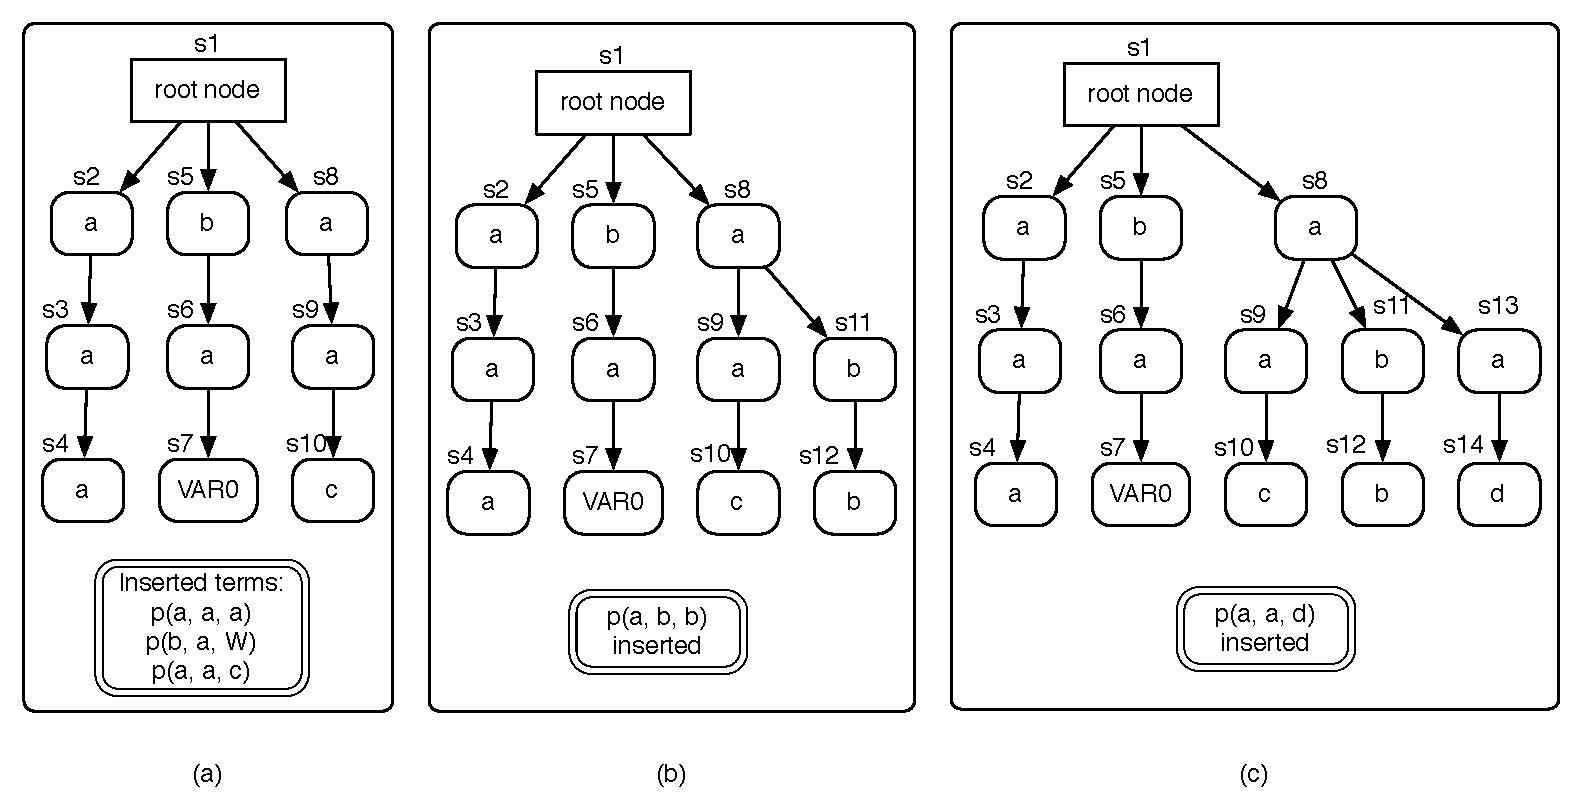
\includegraphics[scale=0.6]{sfa.pdf}
  \caption{Inserting answer terms in a SFA.}
  \label{fig:sfa_example}
\end{figure}

To insert a new term into a SFA, we must start by inserting symbols from the answer term into the root state.
In each state we verify if the last transition $s$ matches the current term symbol $t$. If $t$ matches $s$
we take the transition and advance to the next state; if not, a new transition for $t$ is created and we advance
to the newly created state. When all term symbols $t$ are exhausted, the current state is marked as a leaf,
representing a new answer.
Figure \ref{fig:sfa_example} represents a SFA for the subgoal \texttt{p(X,Y,Z)} and
illustrates insert operations.

When a new subgoal $G$ subsumed by the subgoal $G'$ is first called, we must determine the assignments
from $G'$ to the sub-terms of $G$, because only variable substitutions are inserted into a SFA.
The assignments are usually stored under the choice point.

For example, if $G'$ is \texttt{p(X,Y,Z)} and $G$ is \texttt{p(a,a,V)}, the variable assignments
are $X = a, Y = a, Z = VAR0$. During unification operations, we must unify the first SFA symbol
to $a$, then to $a$ again, and finally with $VAR0$.
Once a variable is \textit{bound}, subsequent unify operations must unify with the bounded sub-term.

The unification process starts in the root state with an empty \textit{continuation stack}.
When a state $s$ is reached, the leftmost transition that unifies with the current $G$ assignment is chosen,
this is called the \textit{applicable transition}.
Before moving to the next state, we select the next applicable transition and push it on the continuation stack.
If no applicable transitions are available at state $s$ or if an answer was found, we pop a transition from
the stack and use it to search for more answers. Once no more transitions can be taken and the stack is empty, the
search process ends.

Using the SFA in Figure \ref{fig:sfa_example} and the subgoal $G$, \texttt{p(a,a,V)}, the search mechanism starts
at the root state and is ready to retrieve all answers that unify with $G$.
The first applicable transition is $s1 \rightarrow s2$ because it unifies with the first symbol: $a$. The transition
$s1 \rightarrow s5$ can not be pushed into the continuation stack because it does not unify, but $s1 \rightarrow s8$ does.
In state $s2$ only one transition is available, thus nothing is pushed into the stack.
Transition $s2 \rightarrow s3$ unifies with symbol $a$ and we move to state $s3$. Here, the variable $VAR0$ (that represents $V$)
can unify with $a$, thus we can get to state $s4$, arriving at a leaf state and a new answer, \texttt{V = a}.

Next, the process must use the continuation stack to retrieve more answers. Transition $s1 \rightarrow s8$ is popped from the stack
and we arrive at state $s8$ with 3 available transitions. Using the previous rules, a new answer is retrieved,
\texttt{V = c} and the continuation stack contains the transition $s8 \rightarrow s13$.

Finally, once states $s8$, $s13$ and $s14$ are visited, the process arrives at a leaf state and a new answer, \texttt{V = d}, is retrieved.
The process finishes and every answer that is specific to \texttt{p(a,a,V)} is found.

\subsubsection{Threaded Sequential Automata}

A \textit{Threaded Sequential Automata} extends the SFA with a concept called
\textit{equivalent states}. One state $S1$ is equivalent to state $S2$ if when $S1$ is taken, $S2$ is also
guaranteed to be visited. For example, in Figure \ref{fig:sfa_example}, whenever states $S2$ and $S8$ are
visited, states $S8$ and $S9$ are also guaranteed to be visited, as they denote the same path.

A SFA is converted to a TSA by adding \textit{equivalence links} between equivalent states.
The SFA in Figure \ref{fig:sfa_example} was transformed into a TSA in Figure \ref{fig:tsa_example}.

\begin{figure}[ht]
  \centering
    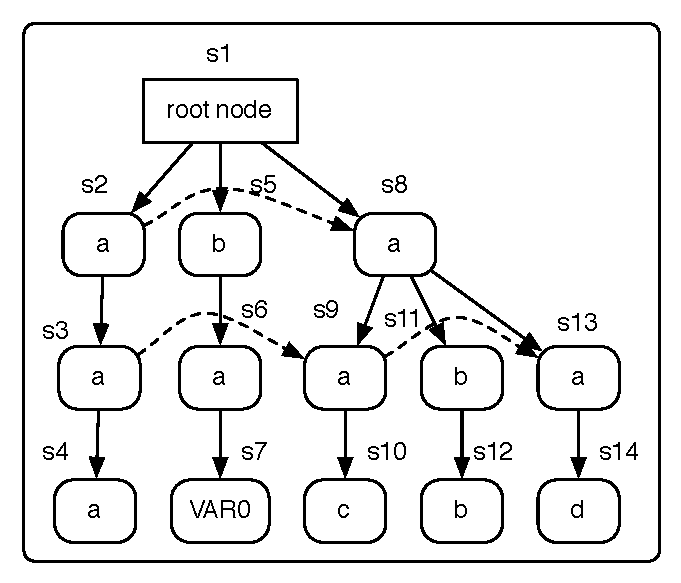
\includegraphics[scale=0.6]{tsa.pdf}
  \caption{SFA transformed into a TSA.}
  \label{fig:tsa_example}
\end{figure}

In the TSA, the concept of applicable transitions is changed. Now it is also possible to push equivalence links
into the continuation stack as if they were normal transitions. So, if we were at state $s3$ we use
the transition to $s9$ and then to $s13$ instead of going from the start state.

Although equivalence links provide an efficient indexing mechanism, they must be used with care. If not,
some situations arise where following equivalence links lead to repeated answers and answers in the incorrect order \cite{Rao-96}.
The selection of transitions must consider only \textit{safe transitions}, which reach answers that cannot be reached through the pending
transitions on the stack.
So, if the process is at state $s2$ and the transition $s1$ to $s8$ is already on the
stack, we can not use the equivalence link $s2$ to $s8$, as the transition $s1$ to $s8$ already covers the same branch.

If we followed only safe transitions, no equivalence links would be used, hence we must check if there is any
equivalence link that can be used in the next state that covers the same answers if we pushed the
usual next applicable transition into the stack. Thus, at state $s2$ we would use the equivalence $s2$ to $s8$, instead of
the transition $s1 \rightarrow s8$.

\begin{figure}[ht]
  \centering
    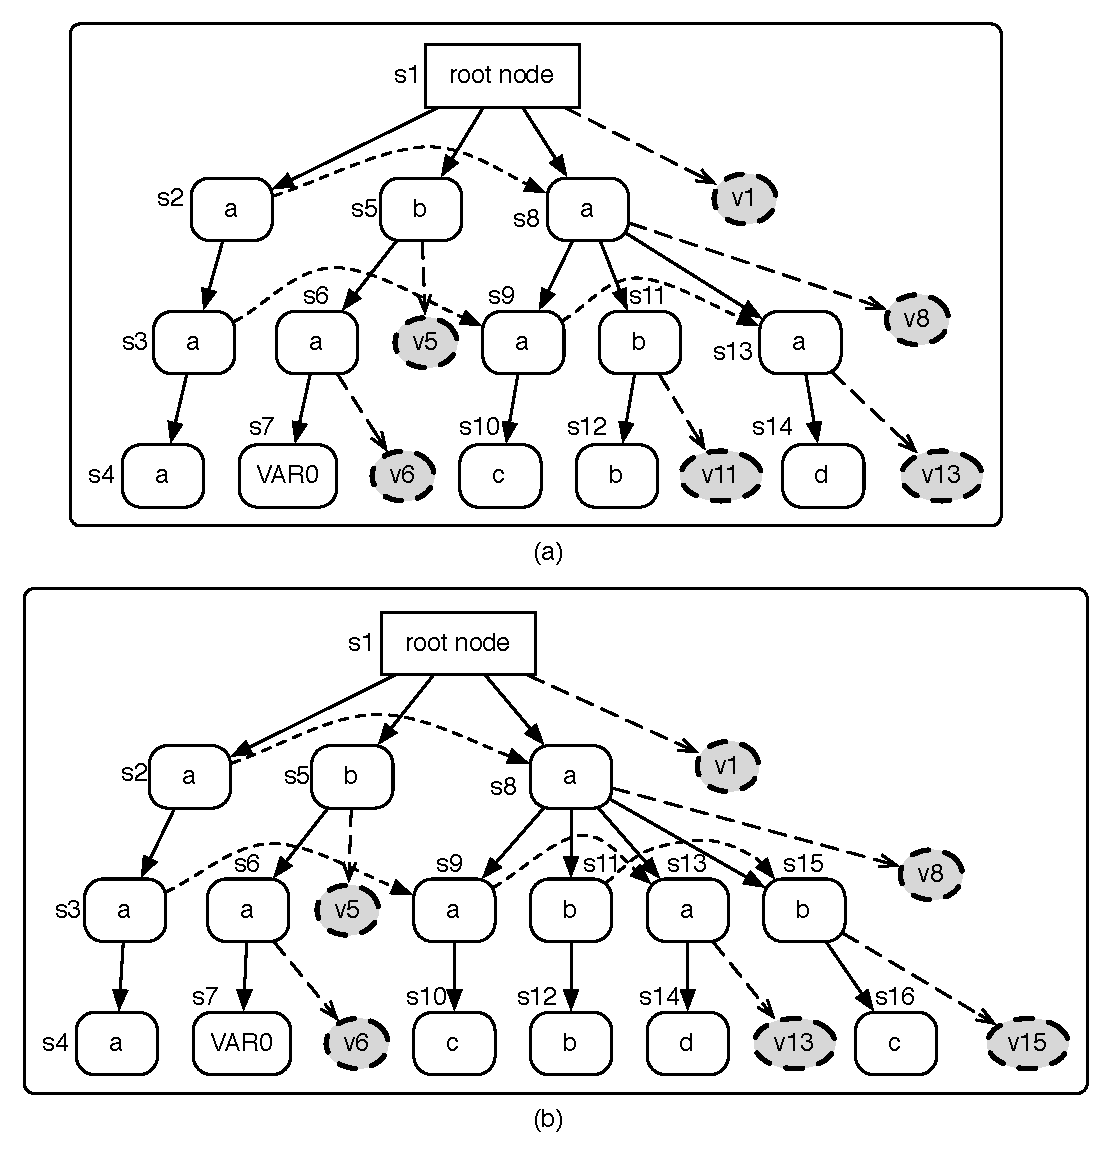
\includegraphics[scale=0.6]{dtsa.pdf}
  \caption{DTSA before and after inserting answer \texttt{p(a,b,c)}.}
  \label{fig:dtsa_example}
\end{figure}
 
\subsubsection{Dynamic Threaded Sequential Automata}

The previously described mechanisms only work if we have the complete set of answers for the subsuming subgoal.
A new mechanism that deals with incomplete answer sets must be devised, so that after all current answers
are retrieved, the continuation stack can be used to retrieve newly inserted answers.

The Dynamic Threaded Sequential Automata extends the TSA with special transitions in states
were new transitions can be inserted or in states were no equivalence links exist.
Figure \ref{fig:dtsa_example} illustrates two DTSAs: (a) shows the converted TSA from Figure \ref{fig:tsa_example}, and
(b) the resulting DTSA after inserting the answer \texttt{p(a,b,c)}.

During answer retrieval, if no answer is found and the top of the continuation stack contains
a transition to a special state, the process stops and the continuation stack is saved along the last state
visited.
Later on, when new answers must be retrieved, the last state is used to transform the stack to account for new states that
were introduced during the insertion of new terms. If the new stack contains a valid transition, it
can now be used as usual.

For example, retrieving answers to subgoal \texttt{p(a,X,c)} from the DTSA (a) in Figure
\ref{fig:dtsa_example} results in the answer \texttt{p(a,a,c)} and a continuation formed by the last
visited state $s13$ and the stack containing (from bottom to top): $[s1 \rightarrow v1, s8 \rightarrow v8, s13 \rightarrow v13]$.
After the new answer \texttt{p(a,b,c)} is inserted into the DTSA in Figure \ref{fig:dtsa_example} and
a consumer is resumed to consume new answers, it checks if new answers are available and the continuation stack
is thus transformed by using the last visited state $s13$ into: $[s1 \rightarrow v1, s8 \rightarrow s15]$. Now
the answer \texttt{p(a,b,c)} can be easily retrieved using the transition $s8 \rightarrow s15$.

\subsubsection{Table Space}

This new DTSA mechanism was implemented in XSB by extending the variant engine \cite{Rao-96}.

First, each subgoal frame for generator nodes now contains both an answer trie and a DTSA.
Answer tries are used to check for duplicate answers and the DTSA is created lazily, when a new subsumed node
first appears.

Each subsumed subgoal in the call trie keeps an answer return list that is built using the DTSA technique.
This answer list is used when variant goals of the subsumed goal are called, thus instead of using
the DTSA, answers are retrieved directly by traversing the linked list.

When a subgoal is marked as complete, the DTSA is deleted and the answer trie is converted into WAM instructions, a feature called
\textit{compiled trie code}. Answers for subsumed goals are then retrieved by using trie instructions
through the usual WAM backtracking mechanism.

\subsection{Time Stamped Tries} \label{sec:time_stamped_tries}

\textit{Time Stamped Tries} (TST) is another mechanism that was implemented in XSB
to support tabling by call subsumption \cite{Johnson-99}.

TST is a relatively simple technique based around the idea of augmenting a trie with information about the relative time
its terms were inserted. The time of insertion of each term is called its time stamp and is represented by a
positive integer. The time stamps are then used for incremental answer retrieval.

\begin{figure}[ht]
  \centering
    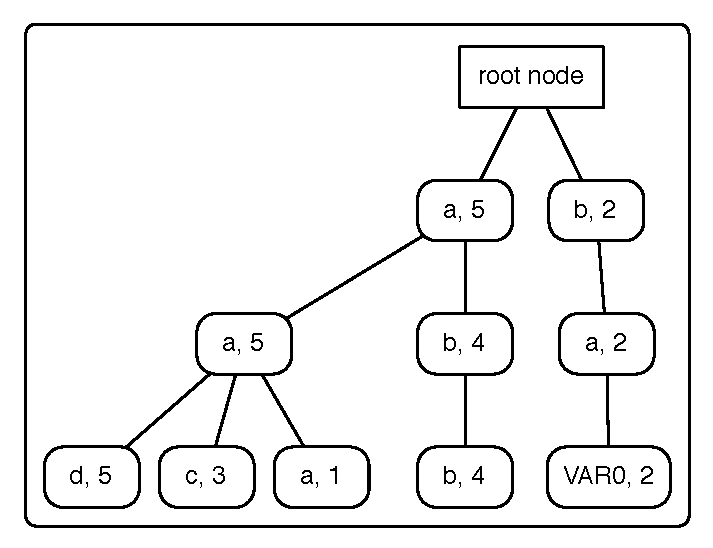
\includegraphics[scale=0.6]{tst_1.pdf}
  \caption{Time Stamped Trie for subgoal \texttt{p(X,Y,Z)}.}
  \label{fig:tst_1}
\end{figure}

For each node in a trie, we extend it by including a time stamp. Along the augmented trie, the maximum time stamp
$T$ is also stored, thus allowing the insert mechanism to know the next time stamp to use for new trie paths.
An example TST for the subgoal \texttt{p(X,Y,Z)} is represented in Figure \ref{fig:tst_1}.
By looking at the leaf nodes, the order of answer insertion
can be readily known: \texttt{p(a,a,a)}, \texttt{p(b,a,VAR0)}, \texttt{p(a,a,c)}, \texttt{p(a,b,b)} and then
\texttt{p(a,a,d)}.

\subsubsection{New Answers}

The process of inserting a new answer into a TST starts by traversing matching nodes as long the stored symbols
match the new answer. If the current symbol does not match, the process changes from search to insert mode and
new nodes are inserted to represent a new trie path. Once the leaf node is created, each node from leaf to root
is traversed and its time stamp is updated to $T + 1$.

\begin{figure}[ht]
  \centering
    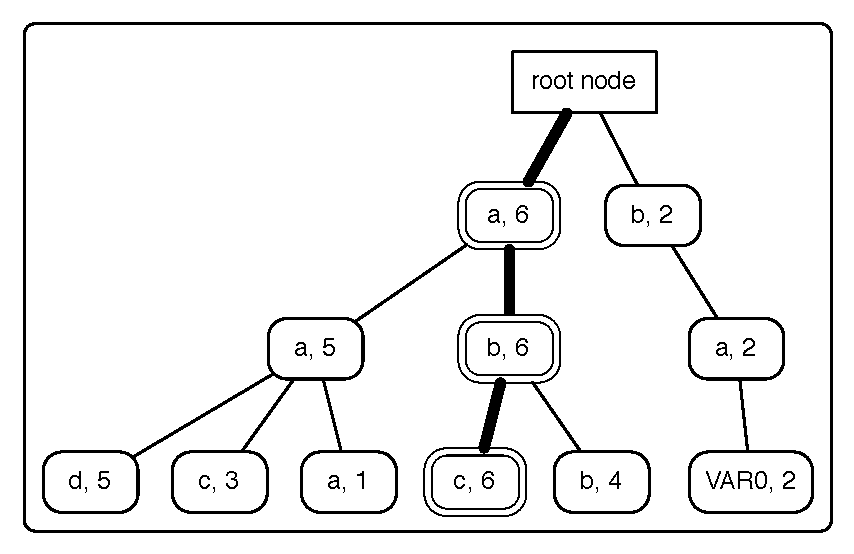
\includegraphics[scale=0.6]{tst_2.pdf}
  \caption{Time Stamped Trie from Figure \ref{fig:tst_1} after inserting the answer \texttt{p(a,b,c)}.}
  \label{fig:tst_2}
\end{figure}

Figure \ref{fig:tst_2} shows the TST from Figure \ref{fig:tst_1} after a new answer \texttt{p(a,b,c)} was inserted.
Note that each node from the answer leaf node to root node was updated with the new timestamp (6). Apart from
the time stamps, search and insertion in TSTs work exactly the same as tries.

\subsubsection{Retrieving Answers}

Retrieving all answers that are specific to a subsumed subgoal $G$ from a TST with answers from subgoal $G'$
works by navigating the TST and unifying the variable values that are assigned from $G'$ to $G$.
If we wanted to retrieve answers to the subgoal \texttt{p(a,a,X)} from the TST in Figure \ref{fig:tst_2},
during the subgoal call we determine the assignments relatively to \texttt{path(X,Y,Z)}: $X = a, Y = a, Z = VAR0$,
and store them under the choice point. Then, these values $[a, a, VAR0]$ are then unified
with the trie symbols, thus finding answers that are specific to $G$.

Like tries, TSTs only store substitutions for variables, thus we must unify
the first sub-term $a$, then $a$ again and then the variable, which unifies with any symbol.
During the unification process, if a variable appears multiple times, it must unify with
any previous sub-term assignment.

Time stamps guide the answer unification process by filtering transitions to already explored branches, where
answers were already retrieved, thus avoiding repeated answers.

The unification process that finds new answers by using a time stamp is separated from the process
of unifying the retrieved answers with the subsumed subgoal. This \textit{two-tier mechanism} is key to the space and time
efficiency of the design of TSTs \cite{Johnson-99} and allows identification of all relevant answers that have
been added since the last time a search operation was done by using the time stamp.

\subsubsection{Table Space}

The table space in this technique extends the variant table space by
using TSTs instead of answer tries for subsuming goals.
 
Each subsumed subgoal in a call trie stores the last search time stamp $t$. The process of
incrementally searching for new answers in a TST will use $t$ and update it after the process completes.
When a subsumptive subgoal is first called $t$ is set to $0$, thus initially allowing the retrieval of all
relevant answers.

The subgoal in the call trie also stores an answer return list. Each time new answers are identified, they are appended
to this linked list. The original subsumptive consumer and its variant subgoals will then consume answers from it. If no
new answers can be retrieved from the list, the TST process is employed to identify more answers from the subsuming TST,
inserting them into the list.

Each TST node maintains a time stamp index which stores all transitions in reverse order.
It is not until a subsumed subgoal is first called that all time stamp related structures are created, thus
allowing a more efficient use of space.

Like DTSAs, the TST indexing mechanism is only used in incomplete subsuming calls, for complete calls
the more specific goals all use compiled trie instructions, and unification is performed naturally at
the WAM engine level.

The biggest advantage of using TSTs instead of DTSAs is in terms of space complexity. In TSTs, the maximum table space
used is at most twice that of the variant engine, because each node must contain both the time stamp and the time stamp index.
For DTSAs, the space used is at least double, but in the worst
case can be quadratic. DTSA is at advantage in terms of speed, because it supports identification of answers and
unification in one step, thus answers can share some elementary unifications. In TSTs, identifying answers
and doing answer unification is a two step process, thus it takes more time to construct all answers. 

\subsection{Finding subsuming goals}

Both DTSA and TST use a similar method that given a call trie $C$ and a subgoal $G$
is able to find a subgoal $G'$ that subsumes $G$.

The search is performed by recursively backtracking through the call trie $C$, trying
to match the node symbols with sub-terms or symbols from $G$.

A non-variable symbol from $G$ must only match with an identical symbol from $C$ and
these types of unifications are always tried first.
If the current trie symbol is a variable, for example $X$, on the first occurrence $X$
is bound to the respective $G$ sub-term
and match succeeds; on the next occurrences of $X$, the current sub-term from $G$ must
be identical to the term bound to $X$. Through the backtracking process, bound variables are
always tried before unbound variables.

Favoring constant values before variables, results in a mechanism that finds \textit{minimally subsuming calls}.
Also, if there is some variant call $G''$ in $C$, $G''$ is found before any other subgoal. If no variant 
or no subsuming call are found, it is possible to save the trie node to insert a new variant call.
This trie node is where the first backtracking occurred or when the first occurrence of
an already seen $G$ variable that could not be paired to a bound trie variable, and instead
must be bound to an unbound trie variable for the process to continue.
The new variant path is then used to keep information about the subsumed goal state in
the leaf call trie node.


\chapter{Time Stamped Tries}
In this chapter, we throughly describe the Time Stamped Tries approach
to implement a subsumptive tabling engine. This mechanism was proposed by
Ernie Johnson \textit{et al} \cite{Johnson-99} and is currently implemented in XSB.
It is based on the idea of extending each answer trie node with \textit{timestamp}
information as a means to identify new answers from old answers.

First, we start by describing the algorithms and data structures associated
with the detection of subsuming goals. Next, we explain the data structures
introduced in the answer tries to support subsumption, focusing on answer insertion
and retrieval for subsumed subgoals. Then, we describe the modifications made in the YapTab
tabling engine to support subsumptive tabling. Finally, we compare the performance of
the subsumptive YapTab against XSB, and the variant counterparts.

\section{Finding subsuming goals}\label{sec:lookup_subsuming}

Both DTSA and TSTs use a similar method that given a call trie $C$ and a subgoal $G$
is able to find a subgoal $G'$ that subsumes $G$.

The search is performed by recursively backtracking through the call trie $C$, trying
to match the node symbols with sub-terms or symbols from $G$. The process stops
once a leaf node is reached successfully.

A non-variable symbol from $G$ must only match with an identical symbol from $C$ and
these types of unifications are always tried first.
If the current trie symbol is a variable, for example \texttt{X}, on the first occurrence \texttt{X}
is bound to the respective $G$ sub-term
and match succeeds; on the next occurrences of \texttt{X}, the current sub-term from $G$ must
be identical to the term bound to \texttt{X}. Throughout the backtracking process, bound variables are
always tried before unbound variables.

Favoring constant values before variables, results in a mechanism that finds \textit{minimally subsuming calls}.
Also, if there is some variant call $G''$ in $C$, $G''$ is found before any other subgoal. If no variant 
or no subsuming call are found, it is possible to save the trie node to insert a new variant call.
This trie node is where the first backtracking occurred or when the first occurrence of
an already seen $G$ variable that could not be paired to a bound trie variable, and instead
must be bound to an unbound trie variable for the process to continue.
The new variant path is then used to keep information about the subsumed goal state in
the leaf call trie node.

\begin{figure}[ht]
  \centering
    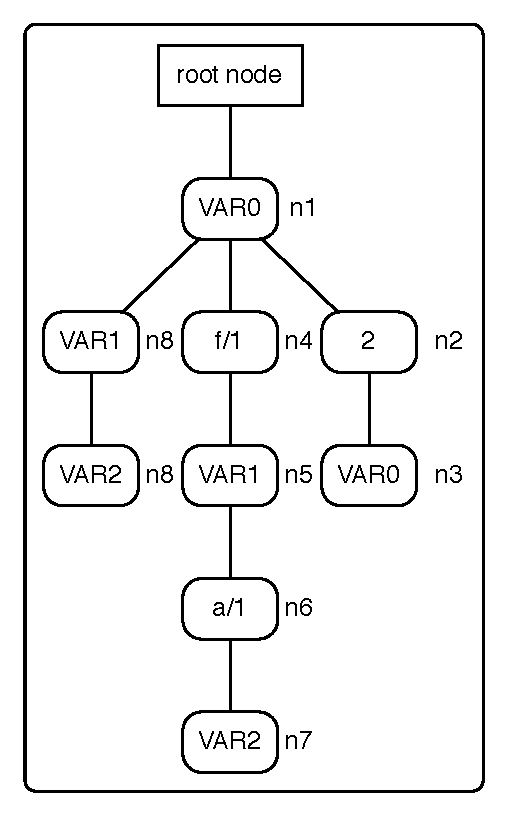
\includegraphics[scale=0.6]{sub_call_search.pdf}
  \caption{Call trie for predicate \texttt{p/3}.}
  \label{fig:sub_call_search}
\end{figure}

For illustration purposes, the Figure \ref{fig:sub_call_search} represents a call trie for the predicate \texttt{p/3}.
The first subgoal called was \texttt{p(X,2,X)}, followed by \texttt{p(X,f(Y),a(Z))} and finally \texttt{p(X,Y,Z)}.

If the subgoal \texttt{p(X,2,X)} is called once again, the algorithm described above
should find the variant subgoal represented by the leaf node $n3$. First, we unify the trie variable
\texttt{VAR0} with \texttt{X} (node $n1$), hence we must also mark the \texttt{X} variable as \textit{seen},
because if the same variable appears again it must unify with the same trie variable for a variant path
to exist. Next, \texttt{2} easily unifies with trie node $n2$ and unification proceeds. In trie node $n3$,
the current call term is \texttt{X} and we also have a variable in the trie node. As \texttt{X} was already seen before,
it must unify with \texttt{VAR0} again, it does and a variant path is found. Please note that if
the trie symbol at node $n3$ was \texttt{VAR1}, the process could proceed but a variant path would be impossible
to exist, and a subsuming subgoal would be found, as \texttt{p(VAR0,2,VAR1)} subsumes \texttt{path(VAR0,2,VAR0)}.
In this case, a variant path could be created by resuming the insert operation at node $n2$ to insert
a \texttt{VAR0} node.

For a more complex example, the subgoal \texttt{p(2,f(X),a(2))} is now called for the same call trie. First,
the algorithm tries to find a trie node with the symbol \texttt{2}, it does not and a variant path
can not be possibly found in this call trie. Next, the algorithm tries to unify with bound variables, but as the process
has just started, only unbound variables can be found and \texttt{VAR0} is unified with \texttt{2} (node $n1$).
The functor term \texttt{f/1} is the next symbol on the subgoal and the first trie node that must be tried is $n4$,
because it contains a non-variable symbol. The next term is \texttt{X} and it can unify with \texttt{VAR1} (node $n5$).
Next, the term symbol \texttt{a/1} matches with trie node $n6$ and the process proceeds. Note that if we failed
at this point, the process would backtrack to node $n2$ and node $n8$ would be tried next, which would
lead to a more general subgoal. Back to node $n6$, the last term symbol \texttt{2} can match with node $n7$, as it is the only trie
node available and it is an unbound variable. If the variable was bound, like \texttt{VAR0} for instance,
the process would check if the current term symbol unifies with the variable binding made before (\texttt{VAR0 = 2}) and
it would also succeed. As node $n7$ is a leaf node, the process finishes and a subsumptive path is found.
The following variable bindings were made: \texttt{VAR0 = 2}, \texttt{VAR1 = X}, and \texttt{VAR2 = 2}.

This algorithm uses various data structures: three auxiliary stacks, a call choice point stack,
a variable bindings vector, and variable enumerator vector. The following summarizes
each data structure: 

\begin{itemize}
  \item \textit{variable bindings vector}: saves bindings for each numbered trie variable. Starts with each position pointing to itself;
  \item \textit{variable enumerator vector}: when a never seen term variable appears it must be bound to a position in this enumerator, ensuring that it can be recognized if it appears a second time;
  \item \textit{term stack}: stores the remaining terms to be unified against trie symbols;
  \item \textit{term log stack}: stores the already matched terms. Each frame contains the top index and the top element of the term stack during frame's creation;
  \item \textit{trail stack}: stores bindings that were made during the process. It is used to untrail variables during backtracking;
  \item \textit{call choice point stack}: used to restore the search process at a certain node to explore alternatives.
\end{itemize}

During execution, two matching methods are considered: the first tries to match exact trie symbols against the current term;
the second method uses trie variables instead of exact symbols and is employed when the first method fails.
When a trie node match succeeds, matching defaults to the first method, which means
that exact matches are always tried before variables when a new \textit{trie level} is reached and variables are mainly
used when backtracking. A trie level represents a set of nodes that are linked by \texttt{sibling} links or are at
the same hash table.

\begin{figure}[ht]
  \centering
    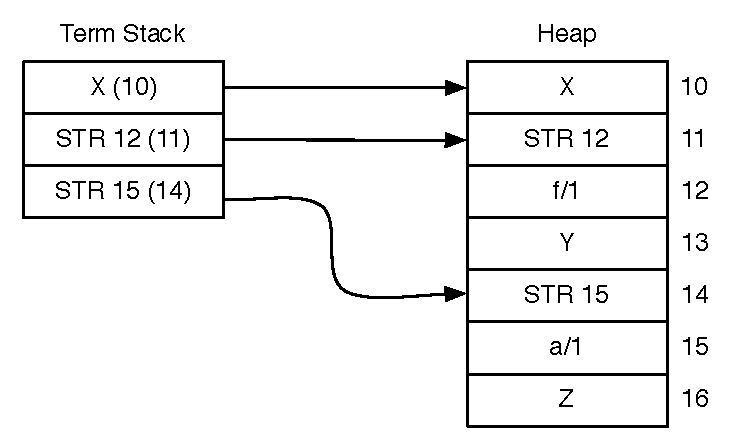
\includegraphics[scale=0.6]{lookup_subgoal_termstack_start.pdf}
  \caption{Initial term stack and heap for subgoal \texttt{p(X,f(Y),a(Z))}.}
  \label{fig:lookup_subgoal_termstack_start}
\end{figure}

The process starts by pushing the $G$ subgoal arguments, $X1, X2, ...Xn$ into the term stack, so that $X1$ is at the top
and $Xn$ at the bottom (Figure \ref{fig:lookup_subgoal_termstack_start}).
Then, the algorithm proceeds in a modified depth-first manner, trying to match the exact nodes first, and then
the variable trie nodes. The skeleton for this algorithm is presented in Figure \ref{fig:lookup_subsuming_call}.

\begin{figure}[ht]
\begin{Verbatim}[fontsize=\small]
lookup_subsuming_call(call_trie, subgoal_call) {
  match_mode = MATCH_EXACTLY
  parent = trie_root(call_trie)
  node = child(parent)
  variable_chain = NULL
  termstack_push_call(subgoal_call)

while_loop:
  while(termstack is not empty) {
    subterm = deref(termstack_pop())
    termstacklog_push(termstack_index(), termstack_top())
  
    if(subterm is atom or integer)
      match_constant(subterm)
    else if(subterm is functor or list)
      match_structured_term(subterm)
    else if(subterm is variable)
      match_variable(subterm)
  
    if(current match failed)
      if(choice point stack is empty) // no more alternatives
        return NO_PATH
      else
        (alt_node, var_chain) = ccpstack_pop_frame()
        match_mode = MATCH_TRIE_VARS
  }
  
  if variant path found
    return (VARIANT_PATH, parent)
  else
    return (SUBSUMPTIVE_PATH, parent)
}
\end{Verbatim}
\caption{Pseudo-code for \texttt{lookup\_subsuming\_call}.}
\label{fig:lookup_subsuming_call}
\end{figure}

\subsubsection{Call choice point stack}

The call choice point stack (Figure \ref{fig:call_choice_point_stack}) contains alternative
search paths to use if the process fails somewhere in the trie.
Each stack frame can restore the search at a given node by restoring all the auxiliary stacks state at the time
of the call frame creation.

\begin{figure}[ht]
  \centering
    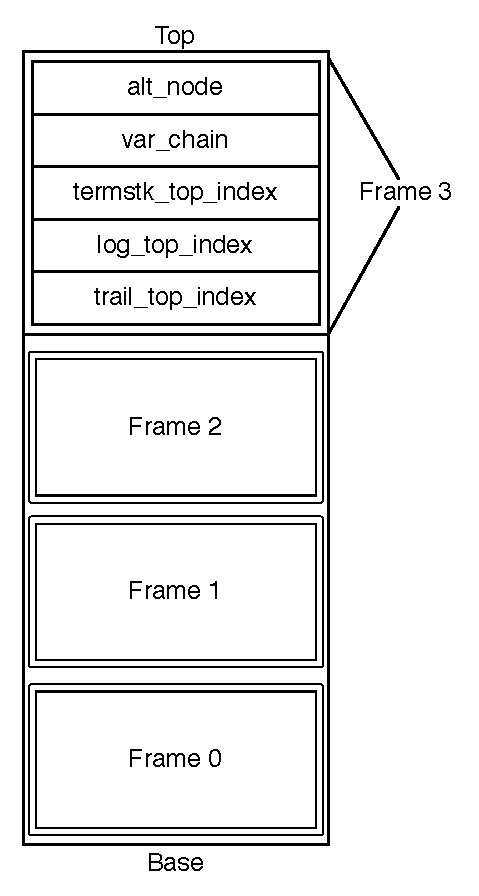
\includegraphics[scale=0.6]{call_choice_point_stack.pdf}
  \caption{Call choice point stack organization.}
  \label{fig:call_choice_point_stack}
\end{figure}

Each frame contains the next trie node to explore (\texttt{alt\_node}),
the current variable chain (\texttt{var\_chain}),
and the following stack indexes during frame creation:
the top of the term stack (\texttt{termstk\_top\_index}),
the top of the term log stack (\texttt{log\_top\_index}),
and the top of the trail stack (\texttt{trail\_top\_index}).
The function \texttt{ccpstack\_push\_frame} (Figure \ref{fig:ccpstack_push_frame})
is used to create a new frame from the computation state.

\begin{figure}[ht]
\begin{Verbatim}[fontsize=\small]
ccpstack_push_frame(alt_node, var_chain) {
  CCPFrame new_frame = new CPPFrame()
  new_frame.alt_node = alt_node
  new_frame.var_chain = var_chain
  new_frame.termstk_top_index = termstack_top - termstack_base + 1
  new_frame.log_top_index = termstacklog_top - termstacklog_base - 1
  new_frame.trail_top_index = trail_top - trail_base
  ccpstack_push(new_frame)
}
\end{Verbatim}
\caption{Pseudo-code for \texttt{ccpstack\_push\_frame}.}
\label{fig:ccpstack_push_frame}
\end{figure}

When popping a frame from the stack, the state of the auxiliary stacks and the other data
structures is restored. Consider a computational state $S1$ that pushed unto the stack
the frame $F1$. Given that we are at state $S2$ and we need to backtrack to the previous state, $S1$,
first we need remove $F1$ from the stack and use the frame's information to restore $S1$.

Any terms that were popped from the term stack from $S1$ to $S2$, which were
stored in the term log stack must be restored back into the term stack.
Then, any bindings made from $S1$ to $S2$ must be untrailed, which is
accomplished by \textit{unwinding} the trail stack. The unwind process untrails
any trie variables bound to the trie variable bindings vector
and any term variable which may have been made to point to the variable enumerator. 

Finally the alternative node and
the variable chain at state $S1$ is also restored. All this is accomplished by the
function \texttt{ccpstack\_pop\_frame} (Figure \ref{fig:ccpstack_pop_frame}).

\begin{figure}[ht]
\begin{Verbatim}[fontsize=\small]
ccpstack_pop_frame() {
  CCPFrame top_frame = ccpstack_pop()
  termstacklog_unwind(top_frame.log_top_index)
  termstack_set_top_of_stack(top_frame.termstk_top_index)
  trail_unwind(top_frame.trail_top_index)
  
  return (top_frame.alt_node, top_frame.var_chain)
}
\end{Verbatim}
\caption{Pseudo-code for \texttt{ccpstack\_push\_frame}.}
\label{fig:ccpstack_pop_frame}
\end{figure}

The node associated with $S2$ and its successors are never visited again and
the process continues until a leaf node is reached or the call choice point stack
is exhausted and the entire trie is visited, yielding no results.

\subsubsection{Matching constants}

The \texttt{match\_constant} function is called when the next term from the term stack is a integer or an
atom. First, in phase \textbf{(1)}, the function checks if the match method is to exactly match the
subterm constant against a trie symbol, which means
that this is the first time this trie level is explored. If the current trie level is represented by a simple
linked list, both \texttt{node} and \texttt{var\_chain} point to the start of the chain, but if the trie level
is an hash table, \texttt{node} will point to the symbol bucket and \texttt{var\_chain} to the variable
bucket, which usually is the first bucket.

\begin{figure}[ht]
\begin{Verbatim}[fontsize=\small]
match_constant(constant) {
  if match_mode == MATCH_EXACTLY // (1)
    (node, var_chain) = set_node_and_var_chain(constant)
    match_node = find_matching_node(constant, node)
    if match_node is not NULL
      conditionally_create_choice_point(var_chain)
      descend_node(match_node)
    else // no match found
      node = var_chain
      no_variant_found(parent)
  // no exact match, try bound trie variables (2)
  match_node = find_bound_trie_var(constant, node)
  if match_node is not NULL
    ccpstack_push_frame(next(match_node), var_chain)
    descend_node(match_node)
  // no bound trie variable found, use unbound trie variables (3)
  match_node = find_unbound_trie_var(var_chain)
  if match_node is not NULL
    bind_trie_var(match_node, constant)
    descend_node(match_node)
}
\end{Verbatim}
\caption{Pseudo-code for \texttt{match\_constant}.}
\label{fig:match_constant}
\end{figure}

The function \texttt{find\_matching\_node} iterates a linked list and locates a trie node that contains the
\texttt{constant} symbol. If this node is found we conditionally create a
new choice point (Figure \ref{fig:conditionally_create_choice_point}), that is
we try to find a node with a variable that can be used when backtracking. At this point, only
trie variables can be explored as only one node with the matched symbol exists at this level.

\begin{figure}[ht]
\begin{Verbatim}[fontsize=\small]
conditionally_create_choice_point(var_chain) {
  foreach(node in var_chain)
    if(is_trie_var(node))
      ccpstack_push_frame(node, node)
      return
}
\end{Verbatim}
\caption{Pseudo-code for \texttt{conditionally\_create\_choice\_point}.}
\label{fig:conditionally_create_choice_point}
\end{figure}

Please note that the found variable node is used as the alternative node in this choice point
and as the variable chain, which will be used to try bound and unbound trie nodes, when backtracking happens.

To descend into a node when a matching succeeds the function \texttt{descend\_node} (Figure \ref{fig:descend_node})
is used. It sets the current \texttt{node} and \texttt{parent} information, sets the matching mode for a new trie level
and changes the program flow to the main \texttt{lookup\_subsuming\_call} while loop. But,
if an exact match fails, we know that the current path cannot be variant of the called subgoal, and we call
\texttt{no\_variant\_found} with the parent node as argument.

\begin{figure}[ht]
\begin{Verbatim}[fontsize=\small]
descend_node(target_node) {
  parent = target_node
  node = child(target_node)
  match_mode = MATCH_EXACTLY
  goto while_loop
}
\end{Verbatim}
\caption{Pseudo-code for \texttt{descend\_node}.}
\label{fig:descend_node}
\end{figure}

Phase \textbf{(2)} of \texttt{match\_constant} can be reached by a failed exact match or by backtracking
(remember that the match mode changes to \texttt{MATCH\_TRIE\_VARS} when backtracking). In this step
we call \texttt{find\_bound\_trie\_var} that will iterate over the \texttt{node} chain to look for
\textit{bound trie variables}. When inserting new subgoals on the call trie, each new trie variable
along a path is marked, so it is easy to check for old variables, which have already been bound
to some term before arriving at the current node. The variable binding can be retrieved by
checking the trie variable bindings position for this variable number, which points to an heap term.
Given that we are trying to match a constant symbol, we verify if the bound term matches our symbol.
In this case, we create a new choice point for the sibling node of the matched trie variable, and use
the currently set variable chain.

Finally, if phase \textbf{(1)} and \textbf{(2)} fail, we try to match our constant against an unbound trie variable
(Figure \ref{fig:find_unbound_trie_var}).
Phase \textbf{(3)} can be also reached by a failed exact and bound trie variable match or by subsequent backtrack
attempts. If a node is found, we bind the variable position on the trie variable bindings
vector to point to the new constant. This position is also trailed on the trail stack, so that it can be untrailed
if backtracking is executed.

\begin{figure}[ht]
\begin{Verbatim}[fontsize=\small]
find_unbound_trie_var(var_chain) {
  foreach(node in var_chain)
    if(is_variable(node) and is_new_variable(node))
      return node
}
\end{Verbatim}
\caption{Pseudo-code for \texttt{find\_unbound\_trie\_var}.}
\label{fig:find_unbound_trie_var}
\end{figure}

\subsubsection{Matching structured terms}

When a structured term appears on the term stack, either a functor or a list, the matching process works
just like constants, except the functor or list arguments must be pushed unto the term stack after an exact
match is found (Figure \ref{fig:match_structured_term}).

\begin{figure}[ht]
\begin{Verbatim}[fontsize=\small]
match_structured_term(term) {
  if match_mode == MATCH_EXACTLY // (1)
    (node, var_chain) = set_node_and_var_chain(term)
    match_node = find_matching_node(term, node)
    if match_node is not NULL
      termstack_push_arguments(term)
      conditionally_create_choice_point(var_chain)
      descend_node(match_node)
    else // no match found
      node = var_chain
      no_variant_found(parent)
  // no exact match, try bound trie variables (2)
  match_node = find_bound_trie_var(term, node)
  if match_node is not NULL
    ccpstack_push_frame(next(match_node), var_chain)
    descend_node(match_node)
  // no bound trie variable found, use unbound trie variables (3)
  match_node = find_unbound_trie_var(var_chain)
  if match_node is not NULL
    bind_trie_var(match_node, term)
    descend_node(match_node)
}
\end{Verbatim}
\caption{Pseudo-code for \texttt{match\_structured\_term}.}
\label{fig:match_structured_term}
\end{figure}

Figure \ref{fig:match_functor} shows the evolution of the term stack for finding
a subsuming goal for the subgoal \texttt{p(a,f(b))}. Step \textbf{(1)} shows the initial 
term stack, followed by a match of the term on top of the stack, \texttt{a}, against \textbf{VAR0}.
As it is an unbound trie variable, the first position of the variable bindings vector is
bound to the target term, \texttt{a}.
In step \textbf{(2)}, we try to match the functor \texttt{f/1} against node \textbf{(b)}, but we fail.
Node \textbf{(c)} succeeds as it is an exact match and the functor argument, \texttt{b}, is pushed on
the term stack. In step \textbf{(3)}, \texttt{b} matches against \texttt{b}, and we find a subsuming call:
\texttt{p(VAR0,f(b))}.

\begin{figure}[ht]
  \centering
    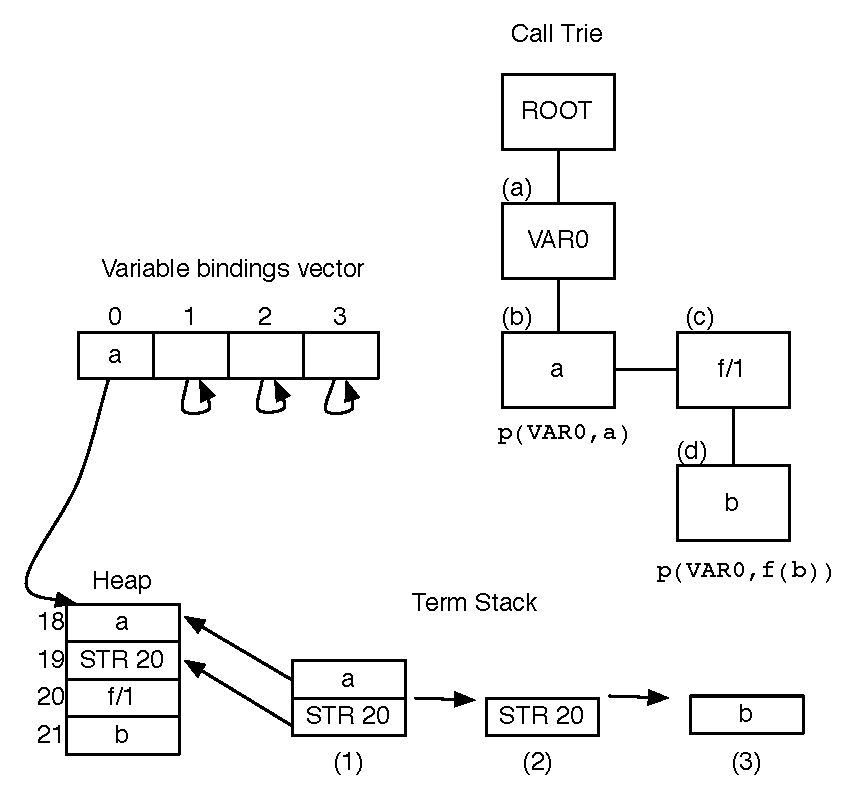
\includegraphics[scale=0.6]{match_functor.pdf}
  \caption{Finding a subsuming goal for subgoal \texttt{p(a,f(b))}.}
  \label{fig:match_functor}
\end{figure}

\subsubsection{Matching variables}

The last case for matching terms are variables. Because we are trying to find a more general goal,
a term variable must only be matched or bound against a trie variable and nothing else. More, a
never seen variable must match only with an unbound trie variable, consider the case of trying to
match \texttt{p(X,Y)} against \texttt{p(X,X)}, the first call variable could match the first trie variable,
but the call variable \texttt{Y} must be matched against an unbound variable, thus the next trie variable
(in this case \texttt{VAR0}) cannot be matched, because it was already bound to another variable.
Please note that \texttt{p(X,X)} is subsumed by \texttt{p(X,Y)} and not the other way around.

To recognize already seen call variables, we bind them to the variable enumerator array, indexed
by the corresponding trie variable number and use the trail stack to trail them.
When such call variable must be matched again with a
trie variable, we first try to match it with the same trie variable, and if we fail to find such trie
variable, we use an unbound trie variable, thus, we avoid binding two different call variables to the same
trie variable.

\begin{figure}[ht]
\begin{Verbatim}[fontsize=\small]
match_variable(term) { // term represents a variable on the heap
  if match_mode == MATCH_EXACTLY
    if node is not NULL and is_hash_table(node)
      node = var_chain = hash_bucket(node, VARIABLE_BUCKET)
    else
      var_chain = node
    if variable is not marked(term)
      // variable not seen before
      // only one new trie variable per level, no choice point needed
      foreach(test_node in node) {
        if is_trie_var(test_node) and is_new_variable(test_node)
          bind_trie_var(test_node, term)
          mark_prolog_var(term, var_index(test_node))
          descend_node(test_node)
      no_variant_found(parent)
      backtrack
  // variable has been seen before
  foreach(test_node in node)
    if is_trie_var(test_node) and !is_new_variable(test_node)
      if identical_terms(trie_var_bindings[test_node], term)
        ccpstack_push_frame(next(test_node), var_chain)
        descend_node(test_node)
  // variant path is not possible here
  no_variant_found(parent)
  // match against unbound trie variable
  foreach(test_node in var_chain)
    // only one new trie variable per level, no choice point needed
    if is_trie_var(test_node) and is_new_variable(test_node)
      bind_trie_var(test_node, trie_var_bindings[prolog_var_index(term)])
      descend_node(test_node)
}
\end{Verbatim}
\caption{Pseudo-code for \texttt{match\_variable}.}
\label{fig:match_variable}
\end{figure}

The pseudo-code to match against a variable is displayed in Figure
\ref{fig:match_variable}. From it, we can conclude that a variant path
cannot be found when: (1) a new trie variable cannot be found
for a new call variable, (2) we cannot match an already seen
call variable against the same trie variable already bound to it.

\subsubsection{Variant continuations}

The \texttt{lookup\_subsuming\_call} algorithm has the ability to find a
minimally subsuming call and if a variant path exists, it will be found.

A \textit{variant continuation} is built when the algorithm detects that a variant path of the
called subgoal cannot be found on the call trie during the search process.
A variant continuation stores all the needed information to later resume
the algorithm that creates a variant path starting from the last node where the
search for a variant path has failed.

In the above pseudo-code we used the function \texttt{no\_variant\_found} to create
a variant continuation. This function creates a continuation the first time it is called.

The continuation stores the node from where the rest of the variant path is created,
the term stack at creation's time and all the bindings made to the call variables
to the variable enumerator vector that were trailed on the trail stack.

\begin{figure}[ht]
  \centering
    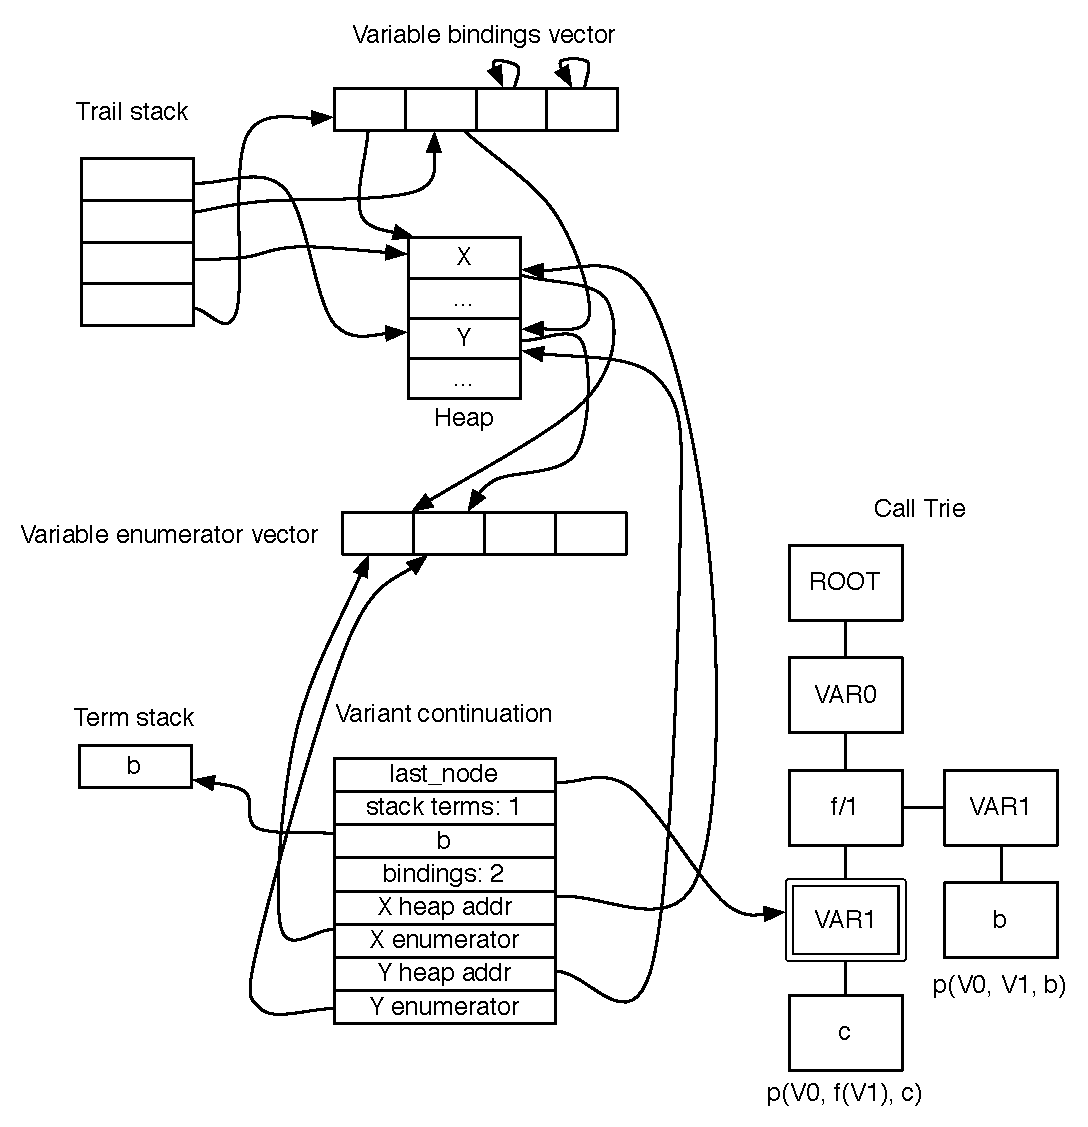
\includegraphics[scale=0.6]{variant_continuation.pdf}
  \caption{Creation of an variant continuation for subgoal \texttt{p(X,f(Y),b)}.}
  \label{fig:variant_continuation}
\end{figure}

Figure \ref{fig:variant_continuation} shows a variant continuation that is built
after the match process failed at node \texttt{c}. If a variant path
for subgoal \texttt{p(X,f(Y),b)} needs to be created: the term stack is restored
with the terms saved on the continuation; the trail stack is initialized with
the two variable heap addresses and each variable is bound to the saved
enumerator addresses. The variable enumerator vector is used during the insertion
of variant paths to detect if a variable was already seen and easily compute its number by
looking at the enumerator position. If it is a new variable, a new trie variable is generated,
and the call variable is pushed on the trail stack and bound to the corresponding enumerator address. 

\section{Answer Templates}

In a variant engine, a substitution factor
represents an array of unique variables which exist in the terms of the argument registers.
These variables are bound to terms when consuming answers from an answer trie.
Figure \ref{fig:answer_template_generator} shows a substitution factor that is constructed
on the local stack below the choice point, in this case a generator choice point.
Note that the substitution factor size (2) is also stored.

\begin{figure}[ht]
  \centering
    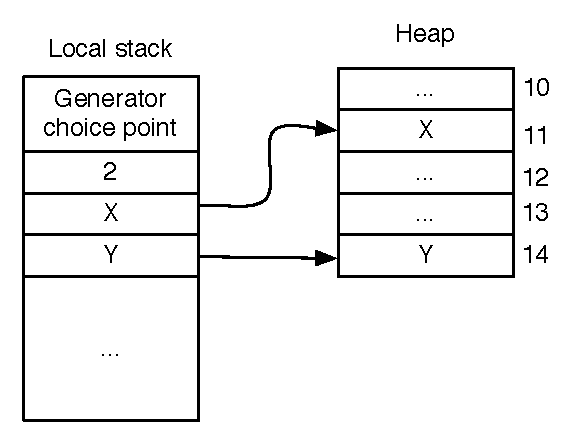
\includegraphics[scale=0.6]{answer_template_generator.pdf}
  \caption{Answer template for generator \texttt{p(X,f(Y))}.}
  \label{fig:answer_template_generator}
\end{figure}

When using call by subsumption, the same factor is used for
subgoals which do not consume from more general subgoals: \textit{generator subgoals}
and variant consumers of generator subgoals.
We call this type of substitution factor a \textit{generator answer template}.

For subgoals with more general subgoals, variants of consumer subgoals and consumers
which consume from consumer subgoals, the answer template must specialize the generator answer template
from the most general subgoal, and is called a \textit{consumer answer template}.
If a generator subgoal \texttt{p(X,f(Y))} exists and the consumer subgoal \texttt{p(a,f(g(2, X)))}
is called, the answer template illustrated on Figure \ref{fig:answer_template_consumer} is built.
Consumer answer templates have the exact same size of generator answer templates
and instead of being composed only of variables, can also be composed with other types of sub-terms.

\begin{figure}[ht]
  \centering
    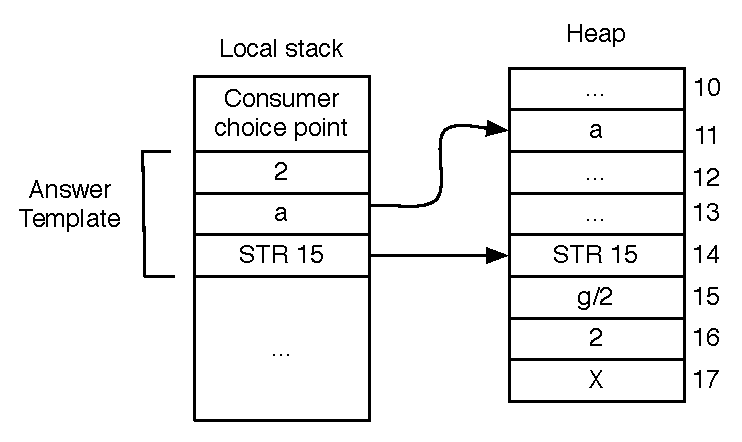
\includegraphics[scale=0.6]{answer_template_consumer.pdf}
  \caption{Answer template for consumer \texttt{p(a,f(g(a,X)))}.}
  \label{fig:answer_template_consumer}
\end{figure}

The construction of answer templates is done when trying to find a general goal on the call trie.
If no subsuming subgoal frame is found, a generator answer template is built. If a subsuming subgoal
is found, the subgoal frame $S$ can be either:

\begin{enumerate}
  \item ... a generator: the answer template is constructed by iterating over the trie variable bindings vector (Figure \ref{fig:extract_template_from_lookup});
  \item ... a consumer: the answer template is reconstructed by using the generator subgoal frame $S'$ from $S$ as we will consume from the generator $S'$ and not $S$. \texttt{reconstruct\_template\_for\_producer} uses another stack, the symbol stack, to push all the trie symbols from the general subgoal path, from leaf to root. The term stack is used to push all the called subgoal arguments that will be matched against the trie symbols. The answer template is then built by matching the new trie variables against the current term on the term stack. Note that when a functor or list symbol appears on the symbol stack the current term is also certainly a functor or list, because the called subgoal specializes the more general subgoal.
\end{enumerate}

\begin{figure}[ht]
\begin{Verbatim}[fontsize=\small]
extract_template_from_lookup(answer_template) {
  total = 0
  foreach(binding in trie variable bindings vector)
    *answer_template-- = binding
    total++
  *answer_template = total
  return answer_template
}
\end{Verbatim}
\caption{Pseudo-code for \texttt{extract\_template\_from\_lookup}.}
\label{fig:extract_template_from_lookup}
\end{figure}

\begin{figure}[ht]
\begin{Verbatim}[fontsize=\small]
reconstruct_template_for_producer(subgoal_call, generator_sf_fr, answer_template) {
  symbol_stack_push_path(leaf_node(generator_sf_fr))
  
  termstack_push_call(subgoal_call)
  
  total = 0
  while(termstack is not empty) {
    subterm = deref(termstack_pop())
    symbol = symbol_stack_pop()
    if is_trie_var(symbol) and is_new_variable(symbol)
      *answer_template-- = subterm
      total++
    else if is_functor(symbol) or is_list(symbol)
      termstack_push_arguments(subterm)
  }
  
  *answer_template = total
  return answer_template
}
\end{Verbatim}
\caption{Pseudo-code for \texttt{reconstruct\_template\_for\_producer}.}
\label{fig:reconstruct_template_for_producer}
\end{figure}

\section{Time stamped tries}

A time stamped node extends an answer trie node with timestamp information, thus
each node contains the following fields: \texttt{symbol}, \texttt{child}, \texttt{parent}, \texttt{sibling}
and \texttt{timestamp}. For implementation and algorithmic purposes, each node also needs a bit field,
\texttt{status}, that describes some node properties that will be described shortly.

Insertion of an answer $S$ into a TST can be divided into two phases:

\begin{enumerate}
  \item Finding a more general answer $S'$ on the trie.
  \item Inserting $S$ if $S'$ could not be found.
\end{enumerate}

Step (1) uses the algorithm described in Section \ref{sec:lookup_subsuming} to discover a more general answer, or,
to find a \textit{repeated answer}, which is a variant of $S$.
Step (2) is executed when (1) fails and uses a variant continuation to resume the insertion of the answer
on the last node a variant answer could be found during the search for $S'$.

\begin{figure}[ht]
\begin{Verbatim}[fontsize=\small]
subsumptive_answer_search(trie_root, ans_vector, maintain_tsi)
  (path, leaf) = lookup_subsuming_call(trie_root, ans_vector) // step 1
  if path == NO_PATH
    // step 2
    leaf = tst_insert(trie_root, restore_variant_continuation(), maintain_tsi)
  return leaf
}
\end{Verbatim}
\caption{Pseudo-code for \texttt{subsumptive\_answer\_search}.}
\label{fig:subsumptive_answer_search}
\end{figure}

The function \texttt{subsumptive\_answer\_search} (Figure \ref{fig:subsumptive_answer_search})
implements the two phase process and needs three arguments: the root of the answer trie \texttt{trie\_root},
the answer as a vector of terms \texttt{ans\_vector}, and a boolean argument, \texttt{maintain\_tsi}.

When a chain of sibling nodes becomes larger then a threshold value, we dynamically index the nodes through an hash table to provide direct node access and therefore optimize the search. Given that an hash table
can have a large number of answer nodes, we maintain a double linked list of answer nodes that we keep on the hash
table, in a decreasing order of the time stamp values. This linked list is called a \textit{time stamped index}.
Besides the usual double linked list pointers, each index node contains a pointer to the answer node
and the timestamp for the answer node. Each answer node indexed in the hash table has a different use
for the \texttt{timestamp} field: instead of containing a positive integer, contains a pointer to the respective index node. Figure \ref{fig:hash_table_tst} illustrates an hash table and its time stamp index.

\begin{figure}[ht]
  \centering
    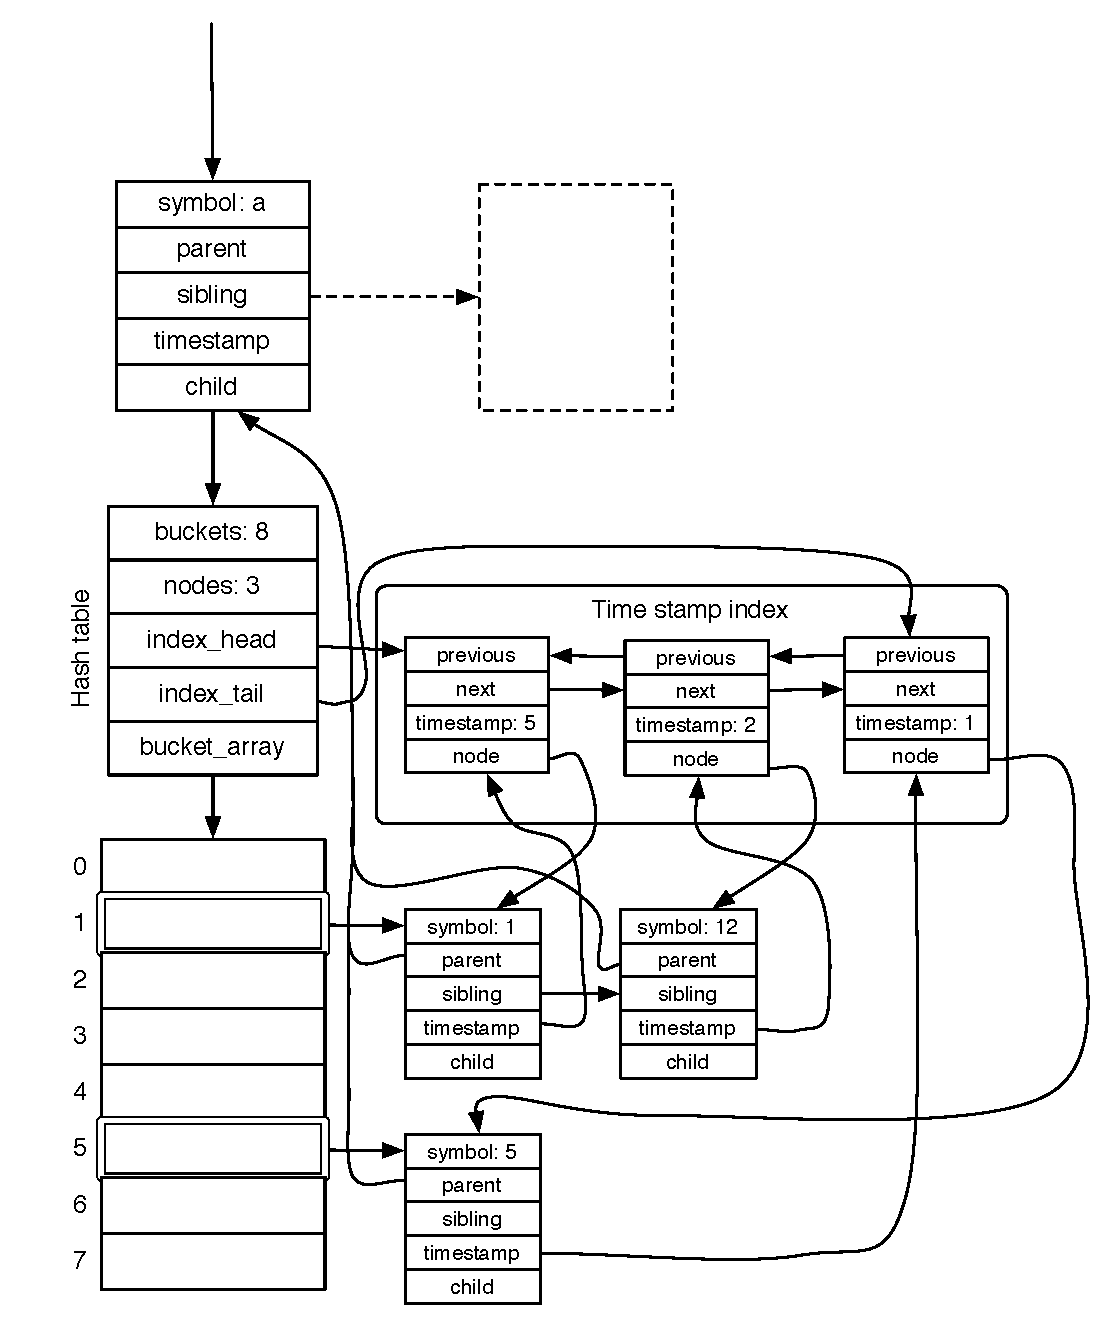
\includegraphics[scale=0.6]{hash_table_tst.pdf}
  \caption{Indexing nodes through an hash table and time stamp indexes.}
  \label{fig:hash_table_tst}
\end{figure}

The argument \texttt{maintain\_tsi} on \texttt{subsumptive\_answer\_search} indicates wether
time stamp indexes exist on the trie and if they need to be maintained.

\subsubsection{Inserting new answers}

Once the variant continuation is restored, the rest of the answer path can be inserted on the trie starting
from the restored node. Inserting is then a simple operation because no checking for equal trie symbols is required.
The first symbol will be inserted either: (1) into a childless parent (ie, the trie root); (2) into a node where
we must append the new node in the sibling chain list; (3) into an hashed node, where the symbol must go be indexed.
Every other symbol will be inserted on a childless parent.

\begin{figure}[ht]
\begin{Verbatim}[fontsize=\small]
tst_insert(trie_root, node, maintain_tsi) {
  symbol = process_term_stack()
  if child(node) == null
    // inserting on the root
    node = tst_add_symbol(node, symbol)
  else if is_hash_table(node)
    node = tst_hash_table_add_symbol(node, symbol, maintain_tsi)
  else
    node = tst_insert_symbol(node, symbol, maintain_tsi)
  
  // at this point, just add nodes on childless parents
  while(termstack is not empty) {
    symbol = process_term_stack()
    node = tst_add_symbol(node, symbol)
  }
  
  update_timestamps(node, trie_root, maintain_tsi)
  return node
}
\end{Verbatim}
\caption{Pseudo-code for \texttt{tst\_insert}.}
\label{fig:tst_insert}
\end{figure}

Function \texttt{tst\_insert} (Figure \ref{fig:tst_insert}) does the job of inserting
all the terms contained in a stack of terms into the trie, starting from \texttt{node}.
The difference between functions \texttt{tst\_add\_symbol} and \texttt{tst\_insert\_symbol}
is that the former inserts symbols on childless nodes and the later on nodes with children.

The function \texttt{process\_term\_stack} pops a term from the term stack and converts the term
to a trie representation, which is usually called a \textit{symbol}. If the term is a functor or a list,
the arguments are pushed into the stack of terms, to be processed next.

\begin{figure}[ht]
  \centering
    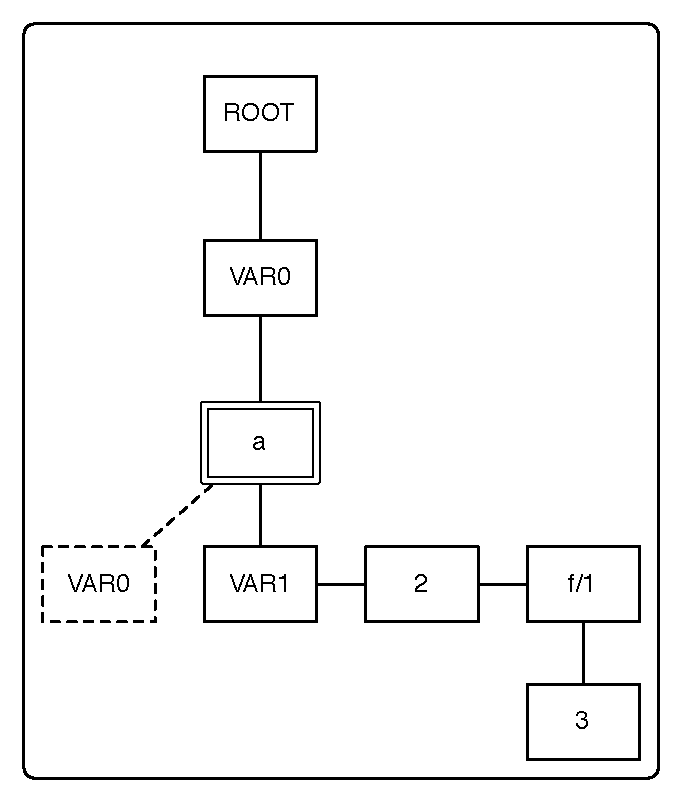
\includegraphics[scale=0.45]{tst_insert.pdf}
  \caption{Inserting answer $\{$\textit{VAR0, a, VAR0}$\}$.}
  \label{fig:tst_chain_insert}
\end{figure}

While appending a new node in a sibling listdoes not involve any
time stamp index (see Figure \ref{fig:tst_chain_insert}), indexing a new node into an hash table does,
because hash tables can index nodes by the time stamp. Figure \ref{fig:hash_table_insert}
illustrates the indexing and insertion of a symbol (25) and the creation of the respective
index node. Note that the \texttt{index head} field was changed to point to the new index node, which
is the node with the greatest time stamp.

\begin{figure}[ht]
  \centering
    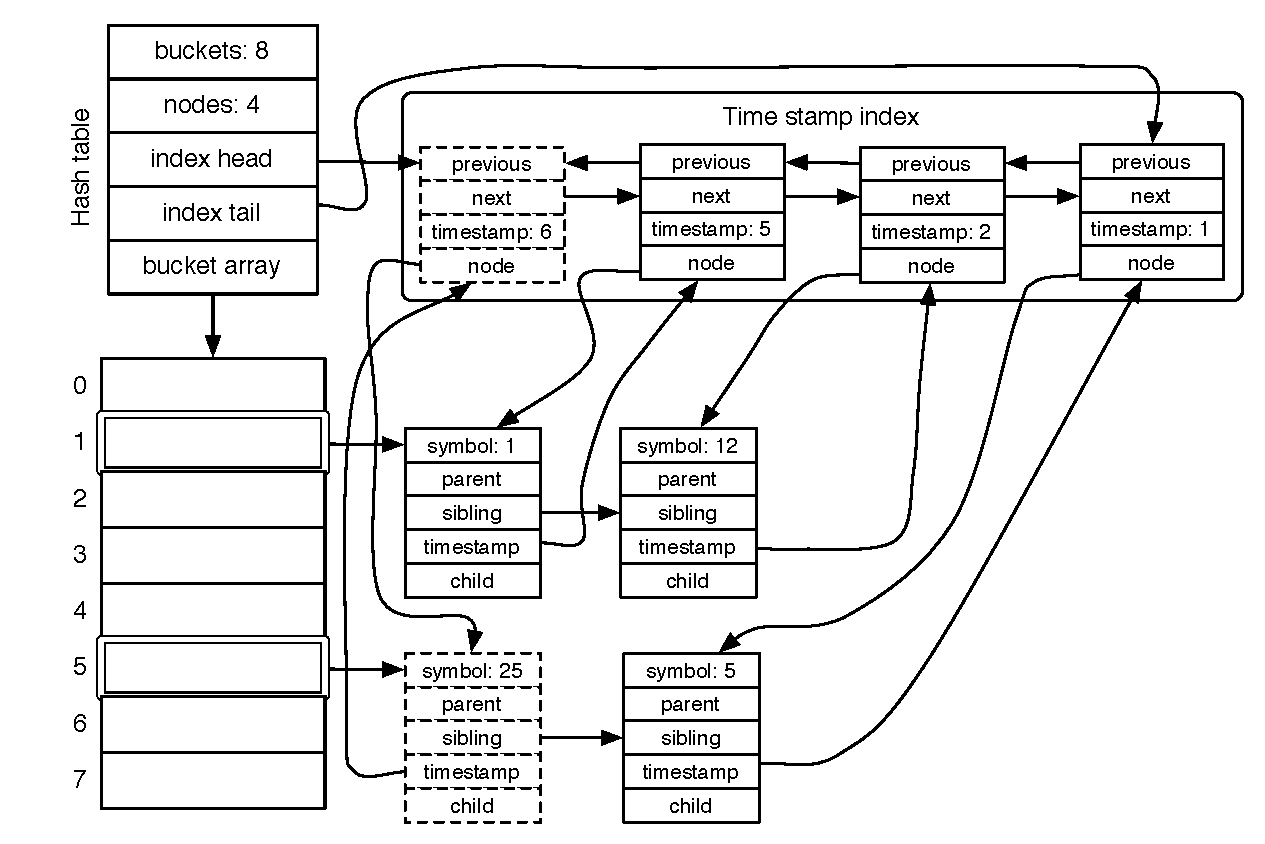
\includegraphics[scale=0.6]{hash_table_insert.pdf}
  \caption{Inserting a node into the hash table and updating the index.}
  \label{fig:hash_table_insert}
\end{figure}

\subsubsection{Updating the time stamps}

Once an answer path is inserted, the time stamps must be updated.
The new time stamp is calculated by inspecting the time stamp of the trie root node.
Next, each path node is navigated using the \texttt{parent} field until reaching the root node.

If the current node is an hashed node and the time stamp indexes
must be maintained, its index node is relocated from its position to the head of the index's double linked list. We can test wether an answer node is indexed by an hash table by inspecting
its \texttt{status} field.

Figure \ref{fig:update_timestamps} contains the pseudo-code for the function \texttt{update\_timestamps}.

\begin{figure}[ht]
\begin{Verbatim}[fontsize=\small]
update_timestamps(leaf, root, maintain_tsi) {
  new_timestamp = timestamp(root) + 1
  
  if(maintain_tsi)
    do {
      if is_hashed_node(leaf)
        // relocate index node
        promote_entry(leaf, new_timestamp)
      else
        timestamp(leaf) = new_timestamp
      leaf = parent(leaf)
    } while leaf != root
  else
    do {
      timestamp(leaf) = new_timestamp
      leaf = parent(leaf)
    } while leaf != root
  timestamp(root) = new_timestamp
}
\end{Verbatim}
\caption{Pseudo-code for \texttt{update\_timestamps}.}
\label{fig:update_timestamps}
\end{figure}

When relocating an index node $N$, the \texttt{index head} of the hash table must be modified
to point to $N$. If the $N$ was at the end of the chain,
the field \texttt{index tail} must be updated to the \texttt{previous} field of $N$.
Previous pointers of the \texttt{next} node of $N$ and the next pointer of
the \texttt{previous} node of $N$ must
also be modified to keep the chain consistent.
Figure \ref{fig:hash_table_promote} illustrates the relocation of an index node, during
the time stamp update to 7.

\begin{figure}[ht]
  \centering
    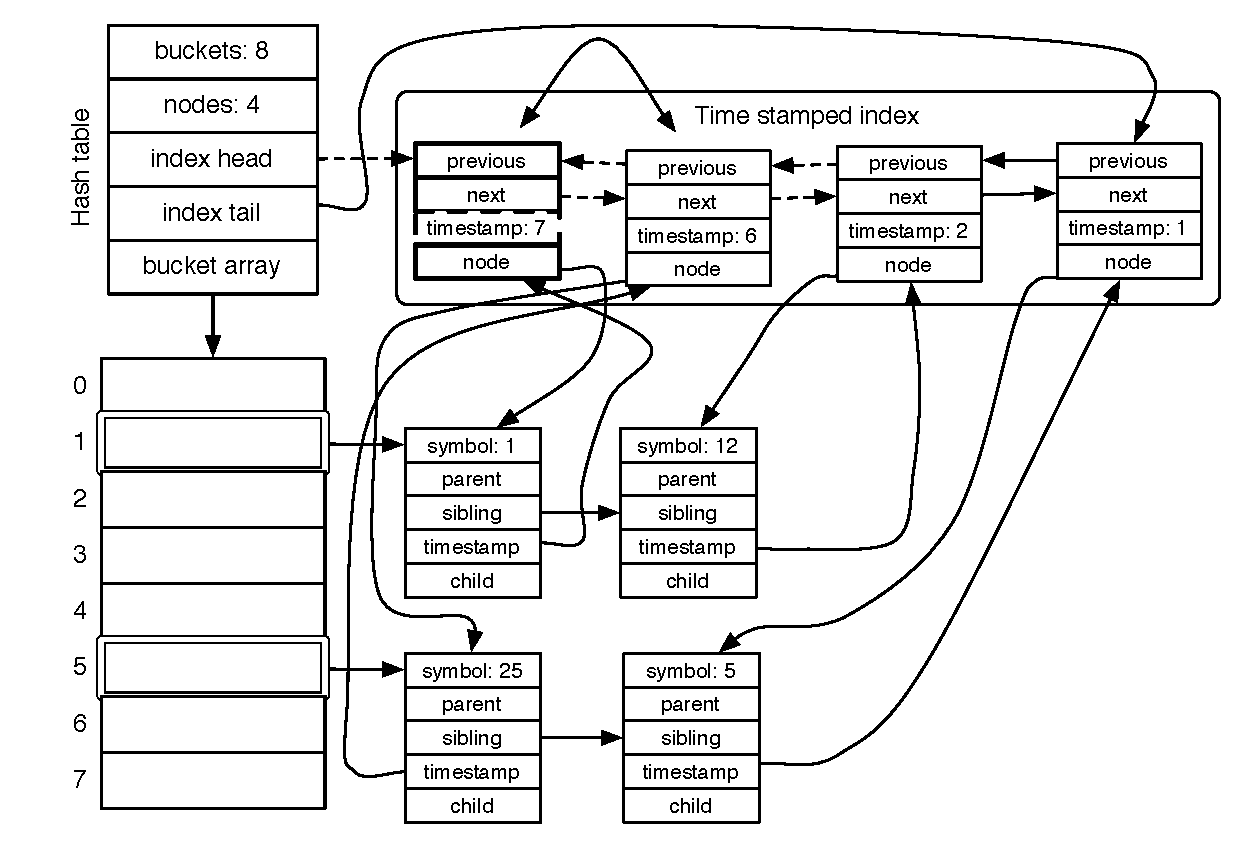
\includegraphics[scale=0.6]{hash_table_promote.pdf}
  \caption{Promoting an index node.}
  \label{fig:hash_table_promote}
\end{figure}

\subsubsection{Lazy creation of time stamp indexes}

Time stamped indexes are only maintained when consumer subgoals are first called.
When the first consumer appears, we must iterate over all the hash tables present
on the trie and create the time stamp index.

To efficiently locate all hash tables in an answer trie, we chain these hash tables
with an extra attribute named \texttt{next}. The start of this chain is stored
as the sibling node of the root answer trie node.

Creating the index for an hash table amounts to iterating over the hashed nodes
and orderly inserting new index nodes on the index chain, as it is being created.

When a subgoal completes, the time stamp indexes, which are only used
during collection of relevant answers
for consumer subgoals, are thrown away to save space.

\section{Collecting Relevant Answers}

The process of collecting relevant answers for a consumer subgoal $G$ from an answer trie $T$
of the generator subgoal $G'$, involves searching $T$ for a set $S$ of answers that unify
with the consumer answer template $AT$ and are newer than time stamp
$TS$ stored in the consumer subgoal frame.
When the process ends, $TS$ is updated to the
timestamp of the root node of $T$, thus avoiding repeated answers in future iterations
of the algorithm. Collected answers are also appended into the list of answers of the consumer subgoal frame, so they can be reused in future calls of $G$.

Various data structures are used for this algorithm, namely:

\begin{itemize}
  \item \textbf{WAM data structures}: the push down list (PDL),
  heap, trail, and associated registers. The heap is used to build complex terms, in which the
  answer template or trie variables are bound. Whenever a variable is bound, we trail it using the WAM trail. The \textit{unify} operation provided by the WAM is used to check for term equality in structured terms;
  
  \item \textbf{term stack}: used to store the next terms to be processed as we navigate through the time stamped;
  
  \item \textbf{term log stack}: when an unification fails, there is a need to backtrack to inspect other branch alternatives, this stack is used to store already processed terms of the term stack, so they can be restored back during backtracking;
  
  \item \textbf{variable bindings vector}: stores binds for trie variables;
  
  \item \textit{choice point stack}: stores choice point frames, where each frame is a search alternative and contains information to restore the state of the computation during the frame's creation.
  
\end{itemize}

The pseudo-code for the algorithm is presented in Figure \ref{fig:tst_collect_relevant_answers}.
It starts by pushing the answer template on the term stack, so that the first component to be unified is at the top. Next, we determine the base trail value by comparing TR against the trail freeze register TR\_FZ, this value can then be used to unbind variables before exiting. The trail register is set to the next free position of the WAM trail, thus avoiding writing on frozen segments. Registers HB, H and TR are saved as they will be manipulated and need to be restored to avoid any interference with the normal WAM execution. Answers gathered during execution are maintained in a linked list of trie leafs and are returned once search is over.

The whole algorithm can be summarized into seven steps:

\begin{enumerate}
  \item Fetch a term $T$ from the term stack;
  \item Search for a node $N$ at the current trie level that: (1) has a valid time stamp (2) unifies with $T$;
  \item Search for the next valid node to be pushed on the choice point stack;
  \item Unify $T$ with the trie symbol of $N$;
  \item Proceed into the child of $N$ or, if step 4 fails, backtrack by popping a frame from the choice point stack and use the alternative node to unify;
  \item Once a leaf is reached, mark a new answer and possibly backtrack to retrieve more answers and go to step (1).
  \item If no more choice point frames exist, return the marked answers.
\end{enumerate}

\begin{figure}[ht]
\begin{Verbatim}[fontsize=\small]
tst_collect_relevant_answers(trie_root, ts, answer_template)
{
  answers = new List()
  
  termstack_push_template(answer_template)
  
  // save WAM registers
  trail_base = TR > TR_FZ ? TR : TR_FZ
  saved_HB = HB
  saved_H = HB = H
  saved_TR = TR
  TR = TR > TR_FZ ? TR : TR_FZ
  
  parent = trie_root
  chain = child(parent)
  
while_loop:
  while(termstack is not empty) {
    subterm = deref(termstack_pop())
    
    if(subterm is atom or integer)
      unify_constant(subterm)
    else if(subterm is functor or list)
      unify_structured_term(subterm)
    else if(subterm is variable)
      unify_variable(subterm)
      
    if choice point stack is empty
      unwind_trail(trail_base)
      restore_wam_registers()
      return answers
    
    choice_point_backtrack()
  }
  
  // new relevant answer found
  list_insert_answer(answers, parent)
  
  // no more choice points?
  if choice point stack is empty
    unwind_trail(trail_base)
    restore_wam_registers()
    return answers
    
  choice_point_backtrack()
  goto while_loop
}
\end{Verbatim}
\caption{Pseudo-code for \texttt{tst\_collect\_relevant\_answers}.}
\label{fig:tst_collect_relevant_answers}
\end{figure}

\subsubsection{Choice Point Stack}

Each choice point frame (Figure \ref{fig:choice_point_stack}) stores the alternative node to explore, the top of the term stack, the top of the term log stack, the current trail position, and the register HB. The HB register serves the same purpose as a WAM choice point saved HB, it is used to store the value of the H register during the choice point creation, so it can restored when backtracking. Figure \ref{fig:cpstack_push_frame} presents pseudo-code for the function \texttt{cpstack\_push\_frame}, which creates a new choice point frame.

\begin{figure}[H]
  \centering
    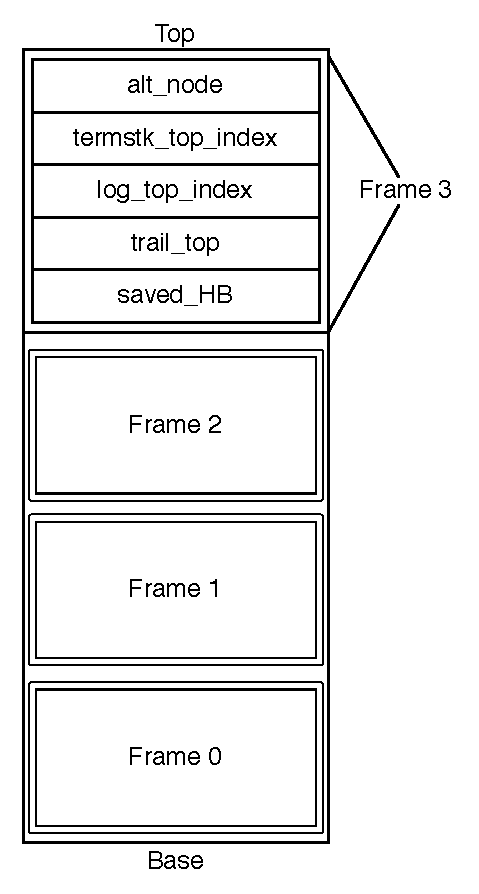
\includegraphics[scale=0.6]{choice_point_stack.pdf}
  \caption{Choice point stack organization.}
  \label{fig:choice_point_stack}
\end{figure}

During execution, the value of the WAM's HB register is compared against the value H to determine if a variable is \textit{conditional}, that is, to determine if a variable needs to be trailed, so that when execution backtracks to a previous choice point we can reset variable bindings. In our case, instead of executing WAM code, we unify a time stamped node, thus the meaning of a conditional variable is extended to include trie variables through the variable bindings vector.

\begin{figure}[H]
\begin{Verbatim}[fontsize=\small]
cpstack_push_frame(alt_node) {
  if alt_node is NULL
    return
  
  CPFrame frame = new Frame()
  frame.alt_node = alt_node
  frame.termstk_top_index = termstack_top() - termstack_base() + 1
  frame.log_top_index = termstacklog_top() - termstacklog_base()
  frame.trail_top = TR
  frame.saved_HB = H
  
  cpstack_push(frame)
}
\end{Verbatim}
\caption{Pseudo-code for \texttt{cpstack\_push\_frame}.}
\label{fig:cpstack_push_frame}
\end{figure}

When a choice point frame is popped from the stack (Figure \ref{fig:cpstack_pop_frame}),
the state of the computation is resumed:

\begin{itemize}
  \item the current node and parent node are reset;
  \item all terms stored in the term log stack are pushed into the term stack;
  \item the trail is unwinded to reset variables that existed during the choice point creation and were bound to terms;
  \item registers H and HB are also reseted to previous values.
\end{itemize}

\begin{figure}[H]
\begin{Verbatim}[fontsize=\small]
cpstack_pop_frame() {
  Frame top_frame = cpstack_pop()
  
  chain = top_frame.alt_node
  parent = parent(chain)
  termstacklog_unwind(top_frame.log_top_index)
  termstack_set_top_of_stack(top_frame.termstk_top_index)
  trail_unwind(top_frame.trail_top)
  H = HB
  HB = top_frame.saved_HB
}
\end{Verbatim}
\caption{Pseudo-code for \texttt{cpstack\_pop\_frame}.}
\label{fig:cpstack_pop_frame}
\end{figure}

\subsubsection{Unify with constant}

Once a trie node $N$ is reached we must select the next trie node $N'$ that unifies with our term and has a valid time stamp. Node $N$ can lead either to a simple node chain or an hash table.
With constant terms we can index the hash table to prune the search space (\texttt{set\_match\_and\_unify\_chains}) by using the \textit{match bucket}.

\begin{figure}[H]
\begin{Verbatim}[fontsize=\small]
unify_constant(constant) {
  if is_hash_table(chain)
    // retrieve the indexed and variable buckets
    (chain, alt_chain) = set_match_and_unify_chains(constant)
    if chain != alt_chain
      search_chain_exact_match(chain, constant, ts, alt_chain)
      // exact match failed
      chain = alt_chain
    if chain is NULL
      backtrack
  search_chain_unify_with_constant(chain, constant, ts)
}
\end{Verbatim}
\caption{Pseudo-code for \texttt{unify\_constant}.}
\label{fig:unify_constant}
\end{figure}

Because variables can unify with the constant term, there is the need to retrieve the variable chain (from the variable bucket), which will be used as the alternative chain to push on the choice point stack. We call it the \textit{unify chain}. If the constant is found on the match chain, the unify chain is used as alternative, but if no match was found, the variable chain will be attempted next and, depending on the remaining nodes, also be used as the backtracking alternative.

\begin{figure}[H]
\begin{Verbatim}[fontsize=\small]
search_chain_exact_match(chain, term, ts, alt_chain) {
  foreach(node in chain) {
    if(term == symbol(node))
      if(valid_timestamp(timestamp(node), ts))
        cpstack_push_frame(chain_next_valid_node(alt_chain, ts))
        termstacklog_push(termstack_index(), termstack_top())
        descend_tst(node)
      else
        return NULL
  }
  return NULL
}
\end{Verbatim}
\caption{Pseudo-code for \texttt{search\_chain\_exact\_match}.}
\label{fig:search_chain_exact_match}
\end{figure}

In Figure \ref{fig:unify_constant} we present the pseudo-code for \texttt{unify\_constant}. Note that we check for an hash table first and inspect the match bucket using \texttt{search\_chain\_exact\_match} (Figure \ref{fig:search_chain_exact_match}).
Finally, if no match is found we set \texttt{chain} to \texttt{alt\_chain} (the unify chain) and execute \texttt{search\_chain\_unify\_with\_constant} on the unify chain. If no hash table was found, we would consider the simple chain of sibling nodes as the unify chain and simply execute \texttt{search\_chain\_unify\_with\_constant}.

\begin{figure}[H]
\begin{Verbatim}[fontsize=\small]
search_chain_unify_with_constant(chain, constant, ts) {
  chain = chain_next_valid_node(chain, ts)
  while(chain is not null) {
    alt_chain = chain_next_valid_node(sibling(chain), ts)
    symbol = trie_deref(symbol(chain))
    if symbol is variable // case (1)
      cpstack_push_frame(alt_chain)
      bind_and_conditionally_trail(symbol, constant)
      termstacklog_push(constant)
      descend_tst(chain)
    else if symbol == constant // case (2)
      // exact match
      cpstack_push_frame(alt_chain)
      termstacklog_push(constant)
      descend_tst(node)
    else
      chain = alt_chain
  }
  // case (3)
}
\end{Verbatim}
\caption{Pseudo-code for \texttt{search\_chain\_unify\_with\_constant}.}
\label{fig:search_chain_unify_with_constant}
\end{figure}

When using a unify chain, we locate the next node with a valid time stamp on the chain, that is, with the time stamp greater than our target time stamp. Next we "dereference" the node symbol by using
\texttt{trie\_deref}, which returns a position on the variable bindings vector if the node symbol is a trie variable, hence allowing trie variables to be used as "normal" variables.

Please note that the function \texttt{bind\_and\_conditionally\_trail} tests if the variable (first argument) is a conditional variable and then trails it using the WAM trail.

In case (1), a variable was found, which can be a position on the variable bindings vector or a prolog variable that was bound to a trie variable; either way, we bind the variable to the constant term, push a new choice point frame with the next valid node, and descend into the child node of \texttt{chain}.

In case (2) the node symbol matches our constant and we simply push a new choice point frame and advance into the next node.

If we could not found a valid trie node in the unify chain, case (3), the next choice point is popped from the choice point stack and the alternative is tried. If the stack is empty, the algorithm finally ends.

As an example, let's consider the time stamped trie in Figure \ref{fig:collect_example_1}. The input answer template is $\{$\texttt{a,b,b}$\}$ and the target time stamp is 3.

\begin{figure}[H]
  \centering
    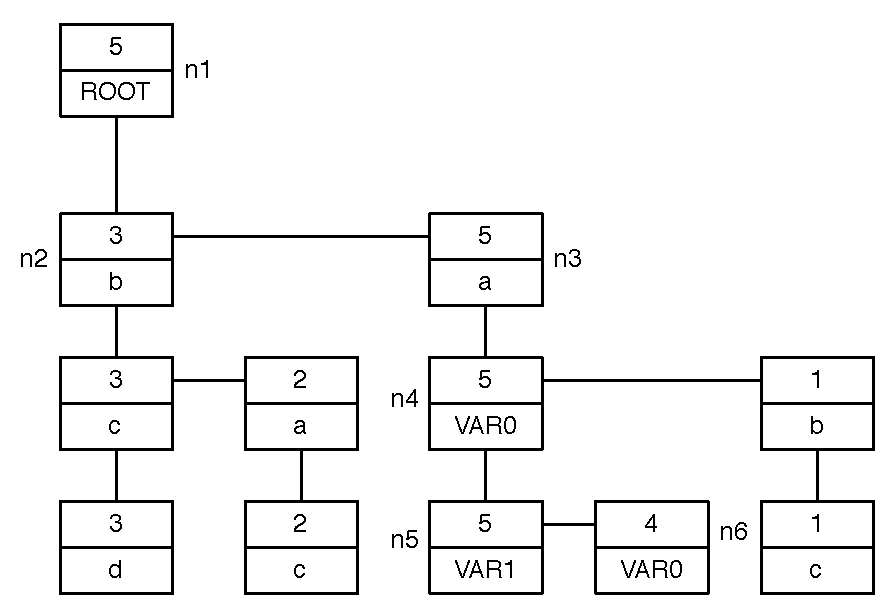
\includegraphics[scale=0.6]{collect_example_1.pdf}
  \caption{Example time stamped trie.}
  \label{fig:collect_example_1}
\end{figure}

We start on node (a) (Figure \ref{fig:collect_ex1}), the root of the trie. The unify chain
is composed by nodes (b) and (c). Node (b) is discarded because the time stamp is invalid.
Node (c) has a valid time stamp and its symbol matches with the current term, \texttt{a}.

\begin{figure}[H]
  \centering
    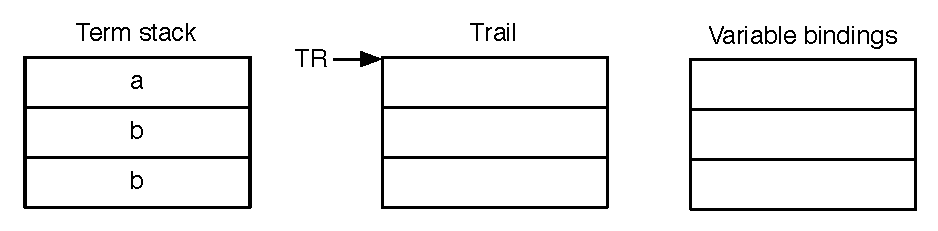
\includegraphics[scale=0.6]{collect_ex1.pdf}
  \caption{At trie node (a).}
  \label{fig:collect_ex1}
\end{figure}

On node (c), our first alternative, node (d) has a valid time stamp and, after doing
\texttt{trie\_deref} we find an unbound variable, \textbf{VAR0}, which is represented
by the first position of the variable bindings vector.
This variable is trailed and bound to \texttt{b},
resulting in what is presented in Figure \ref{fig:collect_ex2}.

\begin{figure}[H]
  \centering
    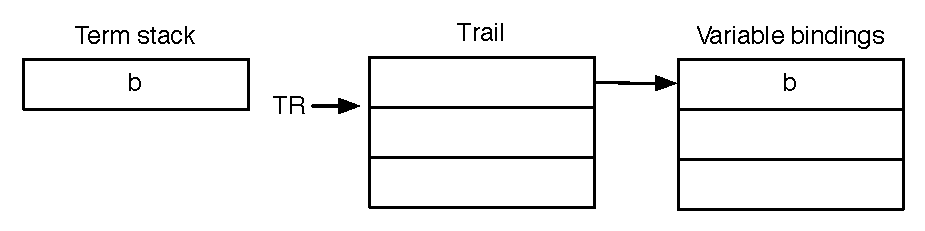
\includegraphics[scale=0.6]{collect_ex2.pdf}
  \caption{At trie node (d).}
  \label{fig:collect_ex2}
\end{figure}

On node (d), the unify chain is composed by nodes (e) and (f). Both have valid time stamps (> 3).
Node (e) is attempted first and easily unifies, because it is an unbound trie variable.
Leaf node (e) is our first answer (Figure \ref{fig:collect_ex3}).

\begin{figure}[H]
  \centering
    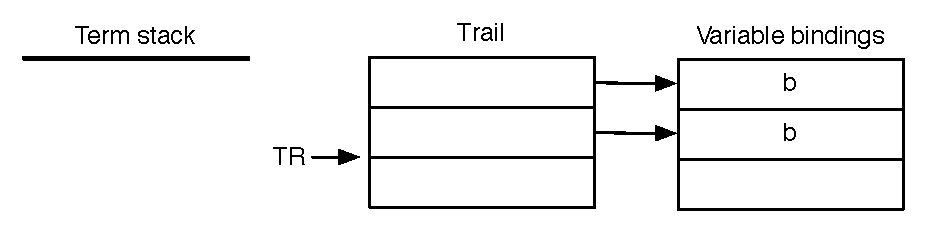
\includegraphics[scale=0.6]{collect_ex3.pdf}
  \caption{At trie node (e).}
  \label{fig:collect_ex3}
\end{figure}

Now, we need to backtrack to collect the other answers. The top choice point frame is retrieved from the stack resulting in a variable being untrailed and the term \texttt{b} being pushed into the term stack (Figure \ref{fig:collect_ex4}).

\begin{figure}[H]
  \centering
    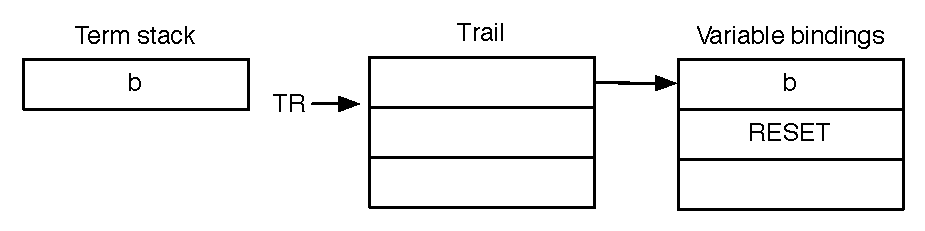
\includegraphics[scale=0.6]{collect_ex4.pdf}
  \caption{Backtracking to node (f).}
  \label{fig:collect_ex4}
\end{figure}

In node (f) we dereference the trie variable \texttt{VAR0} and get the constant term \texttt{b}, which matches the target term. No binding or trailing is needed and we succeed in collecting another relevant answer (Figure \ref{fig:collect_ex5}).

\begin{figure}[H]
  \centering
    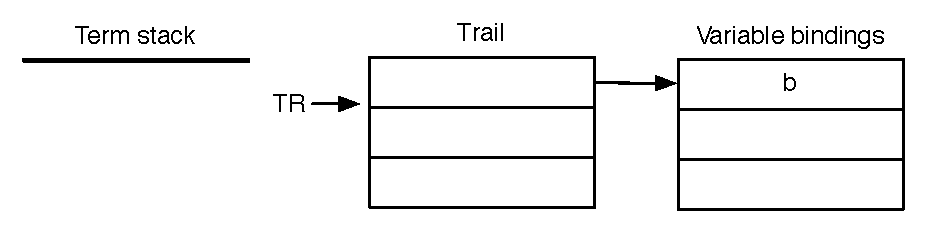
\includegraphics[scale=0.6]{collect_ex5.pdf}
  \caption{New answer as the leaf node (f).}
  \label{fig:collect_ex5}
\end{figure}

As there are no more available choice points we need to untrail any bindings made and return
the answers found (Figure \ref{fig:collect_ex6}), finishing the search.

\begin{figure}[H]
  \centering
    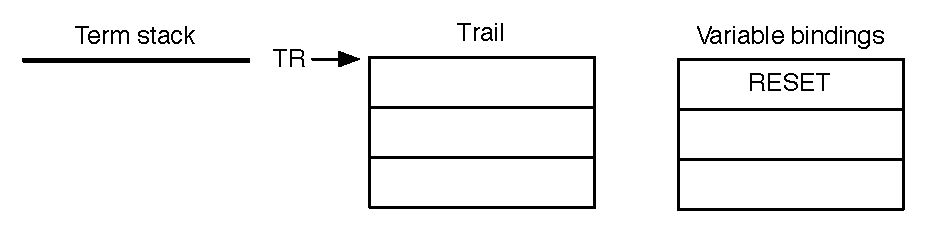
\includegraphics[scale=0.6]{collect_ex6.pdf}
  \caption{Untrailing variables and returning.}
  \label{fig:collect_ex6}
\end{figure}

\subsubsection{Unify with structured term}

For structured terms, the unification process is similar to constant unification. The
current term in the term stack must be a functor or a list. First, we check if the current
trie node is an hash table and the match and unify chains are computed.
If the match chain contains a valid trie node, before we descend into the child
node we must push the functor or list arguments into the term stack, so they can
be unified with the next trie nodes.

\begin{figure}[H]
\begin{Verbatim}[fontsize=\small]
unify_structured_term(term) {
  if is_hash_table(chain)
    // retrieve the indexed and variable buckets
    (chain, alt_chain) = set_match_and_unify_chains(term)
    if chain != alt_chain
      search_chain_exact_match_push(chain, term, ts, alt_chain)
      // exact match failed
      chain = alt_chain
    if chain is NULL
      backtrack
  search_chain_unify_with_structured_term(chain, term, ts)
}
\end{Verbatim}
\caption{Pseudo-code for \texttt{unify\_structured\_term}.}
\label{fig:unify_structured_term}
\end{figure}

When using the unify chain with \texttt{search\_chain\_unify\_with\_structured\_term}
\ref{fig:search_chain_unify_with_structured_term},
we also loop the chain for valid time stamped nodes.
Four situations may arise:

\begin{enumerate}
  \item The current term is variable, which is trail and bound to the structured term;
  \item The trie symbol is a structured term and matches our functor or list.
  The term arguments are pushed into the term stack for unification;
  \item We find a trie variable bound to a structured term. The WAM function \texttt{unify} is executed to check for a match and perform additional unifications;
  \item No match was found, the next alternative node is inspected.
\end{enumerate}

\begin{figure}[H]
\begin{Verbatim}[fontsize=\small]
search_chain_unify_with_structured_term(chain, term, ts) {
  chain = chain_next_valid_node(chain, ts)
  while(chain is not null) {
    alt_chain = chain_next_valid_node(sibling(chain), ts)
    symbol = trie_deref(symbol(chain))
    if symbol is variable // case (1)
      cpstack_push_frame(alt_chain)
      bind_and_conditionally_trail(symbol, term)
      termstacklog_push(term)
      descend_tst(chain)
    else if symbol is a structured term
      if original type of symbol is a structured term and symbol == term
        // case (2)
        cpstack_push_frame(alt_chain)
        termstacklog_push(term)
        termstack_push_arguments(term)
        descend_tst(chain)
      else if unify(term, symbol) // case (3)
        // trie variable bound to an heap structured term
        cpstack_push_frame(alt_chain)
        termstacklog_push(term)
        descend_tst(node)
    else
      chain = alt_chain
  }
  // case (4)
}
\end{Verbatim}
\caption{Pseudo-code for \texttt{search\_chain\_unify\_with\_structured\_term}.}
\label{fig:search_chain_unify_with_structured_term}
\end{figure}

Let's consider the time stamped trie in Figure \ref{fig:collect_functor}
and the following answer template: $\{$\texttt{STR 3, STR 6, STR 9}$\}$.
The target time stamp is 1.

\begin{figure}[H]
  \centering
    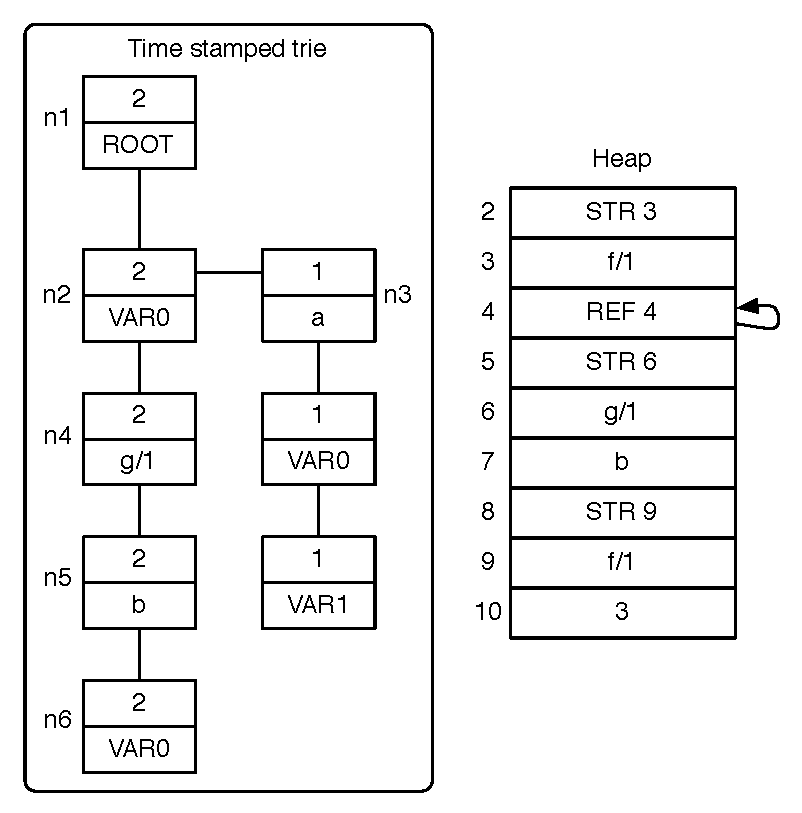
\includegraphics[scale=0.6]{collect_functor.pdf}
  \caption{Example time stamped trie and heap with terms referenced in the answer template.}
  \label{fig:collect_functor}
\end{figure}

At node (a) the term stack contains the full answer template and the variable bindings vector
is empty \ref{fig:collect_functor1}. Only node (b) satisfies the time stamp requirements,
as $2 > 1$.

\begin{figure}[H]
  \centering
    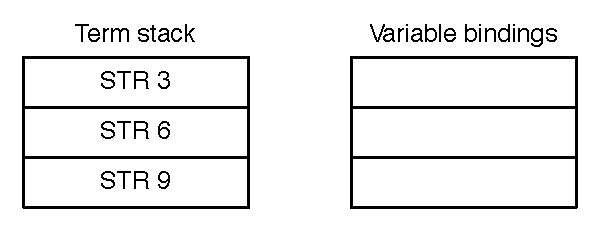
\includegraphics[scale=0.6]{collect_functor1.pdf}
  \caption{Term stack and variable bindings vector at node (a).}
  \label{fig:collect_functor1}
\end{figure}

Node (b) contains a trie variable and the current term is \texttt{STR 3} or \texttt{f(VAR)}.
In this situation, the variable bindings position for \textbf{VAR0} is trailed and bound to \texttt{STR 3}. The data structures configuration is presented in Figure \ref{fig:collect_functor2}.

\begin{figure}[H]
  \centering
    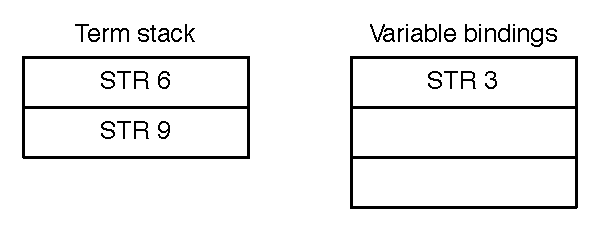
\includegraphics[scale=0.6]{collect_functor2.pdf}
  \caption{Term stack and variable bindings vector at node (b).}
  \label{fig:collect_functor2}
\end{figure}

Node (d) contains the symbol \texttt{g/1} and the current term is \texttt{STR 6}
or \texttt{g(b)}, which matches. The argument \texttt{b} of \texttt{g(b)}
is pushed into the term stack to be processed in the next node (Figure \ref{fig:collect_functor3}).

\begin{figure}[H]
  \centering
    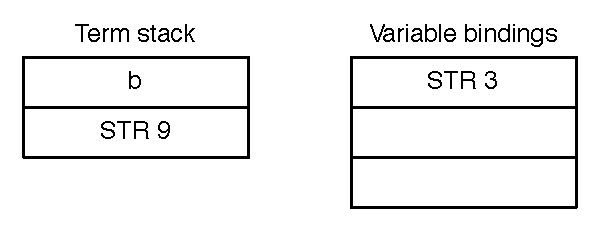
\includegraphics[scale=0.6]{collect_functor3.pdf}
  \caption{Term stack and variable bindings vector at node (d).}
  \label{fig:collect_functor3}
\end{figure}

Node (e) has the symbol \texttt{b} which matches with \texttt{b} from the term stack and
execution proceeds to node (f) (Figure \ref{fig:collect_functor4}).

\begin{figure}[H]
  \centering
    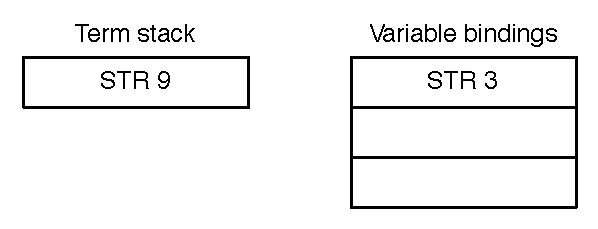
\includegraphics[scale=0.6]{collect_functor4.pdf}
  \caption{Term stack and variable bindings vector at node (e).}
  \label{fig:collect_functor4}
\end{figure}

At (f) we find a trie variable, which, after being dereferenced, contains the
functor \texttt{f(VAR)}. The current term to be unified is \texttt{f(3)}.
In this situation we call \texttt{unify}, which will try to unify both terms.
The unification has the side effect of setting the heap variable cell 4 to \texttt{3}
(Figure \ref{fig:collect_functor5}).
This variable is conditional because it is positioned before the register \texttt{HB},
which given the algorithm design must be greater than 10.

\begin{figure}[H]
  \centering
    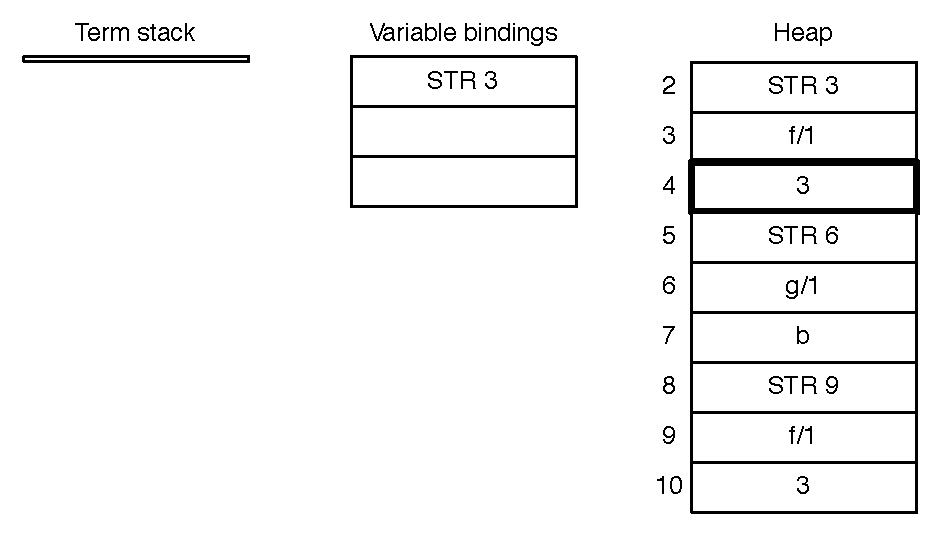
\includegraphics[scale=0.6]{collect_functor5.pdf}
  \caption{Term stack, variable bindings vector and heap at node (f).}
  \label{fig:collect_functor5}
\end{figure}

\subsubsection{Unify with variable}

Because variables unify with anything, when the top of the term
stack is a variable, the next trie branches only need to be pruned using the time stamp.

Figure \ref{fig:unify_variable} presents the function
\texttt{unify\_variable}. Here, we have three cases:

\begin{enumerate}
  \item The current chain link is an hash table. In this situation we can select the next transitions by using the time stamped index, which can easily prune based on the time stamp;
  \item The current node is inside an hash table, thus is on the time stamped index. The node is matched against the variable and the alternative node is selected by following the index chain links;
  \item Current node is a simple sibling chain. Both the chain and the alternative chain are set by iterating over the node chain, looking for valid time stamps.
\end{enumerate}

Once chains are set, we create a new choice point, run the variable unification algorithm
and proceed into the next trie node.

\begin{figure}[H]
\begin{Verbatim}[fontsize=\small]
unify_variable(var) {
  if is_hash_table(chain) // case (1)
    index = index_head(chain)
    if timestamp(index) > ts
      chain = node(index)
      alt_chain = next_valid_index(index, ts)
    else backtrack
  else if is_hashed_node(chain) // case (2)
    // can only be here via backtracking
    alt_chain = next_valid_index(get_index(chain), ts)
  else // case (3)
    // simple chain of siblings
    chain = chain_next_valid_node(chain, ts)
    if chain is NULL backtrack
    alt_chain = sibling(chain)
  
  cpstack_push_frame(alt_chain)
  termstacklog_push(var)
  symbol = trie_deref(symbol(chain))
  unifiy_with_variable(var, symbol, chain)
  descend_tst(chain)
}
\end{Verbatim}
\caption{Pseudo-code for \texttt{unify\_variable}.}
\label{fig:unify_variable}
\end{figure}

From the pseudo-code in Figure \ref{fig:unify_with_variable}, variable unification
must consider the following situations:

\begin{itemize}
  \item symbol is a constant: the term variable is bound to the symbol and conditionally trailed.
  \item symbol is a structured term: if the symbol was a trie variable bound to a term then we bind the variable to the heap location; else, we create a new structure (functor or list) on the heap and bind the variable to it, resulting in a term with various heap variables as arguments, which will be pushed into the term stack and will be bound in the next iterations of the algorithm.
  \item symbol is a variable: if the variable is a trie variable, we bind and trail it; if it is an heap variable that was dereferenced from a trie variable using \texttt{trie\_deref}, \texttt{unify} chooses the binding direction, resulting in one of the variables being trailed.
\end{itemize}

\begin{figure}[H]
\begin{Verbatim}[fontsize=\small]
unify_with_variable(var, symbol, node) {
  if symbol is a constant
    bind_and_conditionally_trail(var, symbol)
  else if symbol is a structured term
    if node symbol is a structured term
      bind_and_conditionally_trail(var, H)
      create_heap_structure(symbol)
      termstack_push_arguments(deref(var))
    else
      // trie variable bound to an heap structure
      bind_and_conditionally_trail(var, symbol)
  else if symbol is a variable
    if symbol is a trie variable
      bind_and_trail(symbol, var)
    else
      // two heap variables
      unify(symbol, var)
  else
    backtrack
}
\end{Verbatim}
\caption{Pseudo-code for \texttt{unify\_with\_variable}.}
\label{fig:unify_with_variable}
\end{figure}

As an example, consider the trie and heap in Figure \ref{fig:collect_variable}.
The input answer template is $\{$\texttt{REF2,REF2,b}$\}$ and the start time stamp is 2.

\begin{figure}[H]
  \centering
    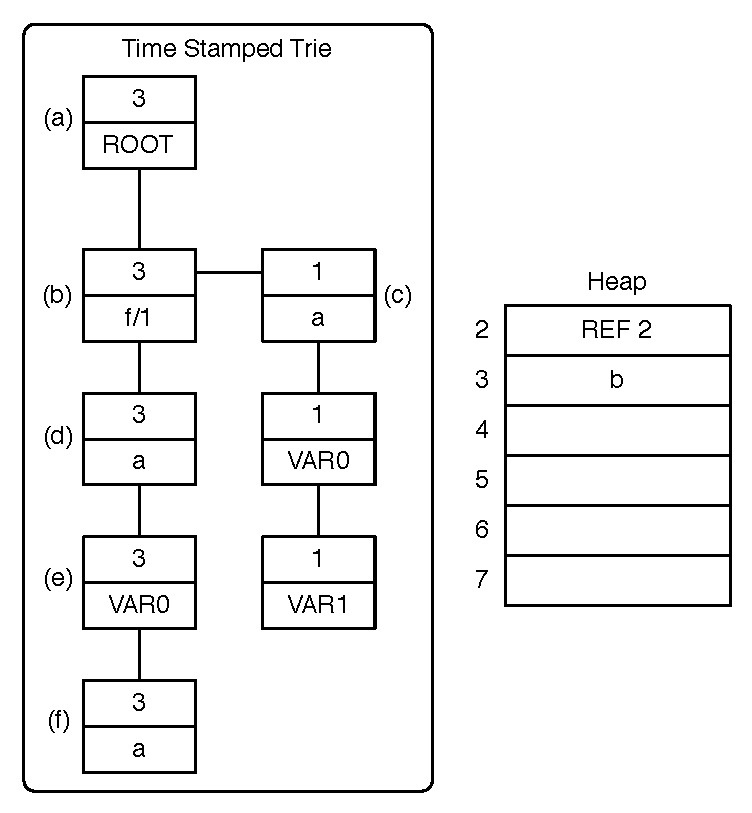
\includegraphics[scale=0.6]{collect_variable.pdf}
  \caption{Example time stamped trie and heap.}
  \label{fig:collect_variable}
\end{figure}

Starting on root node (a), we have the following data structure configuration:

\begin{figure}[H]
  \centering
    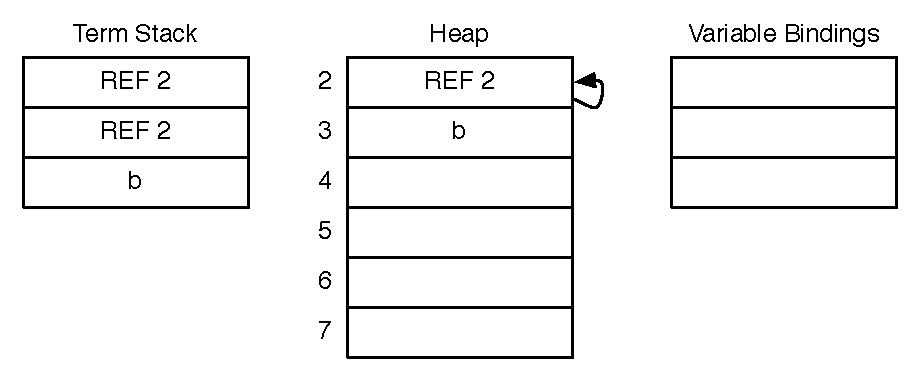
\includegraphics[scale=0.6]{collect_variable1.pdf}
  \caption{At node (a).}
  \label{fig:collect_variable1}
\end{figure}

Node (b) is the only valid transition, with time stamp 3.
The functor \texttt{f/1} is unified against the variable \texttt{REF 2},
which results in the functor \texttt{f/1} being created on the heap
and its argument (\texttt{REF 5}) being pushed into the term stack
(Figure \ref{fig:collect_variable2}).

\begin{figure}[H]
  \centering
    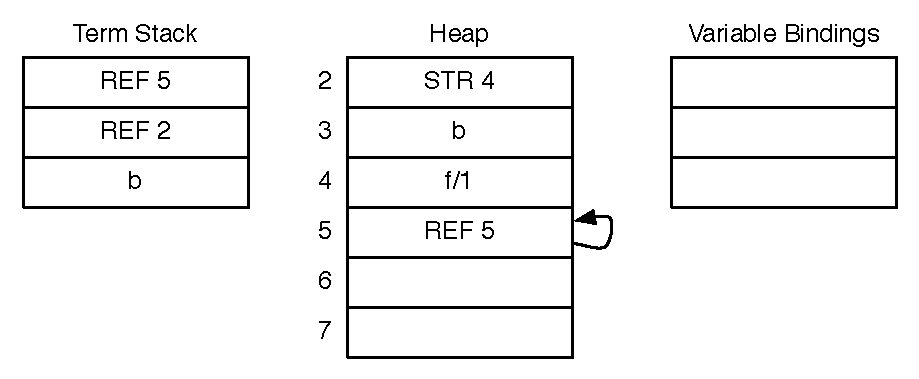
\includegraphics[scale=0.6]{collect_variable2.pdf}
  \caption{After unifying with node (b).}
  \label{fig:collect_variable2}
\end{figure}

The yet unbound functor argument matches atom \texttt{a} in node (d),
resulting in the update of the heap cell 5 (Figure \ref{fig:collect_variable3}).

\begin{figure}[H]
  \centering
    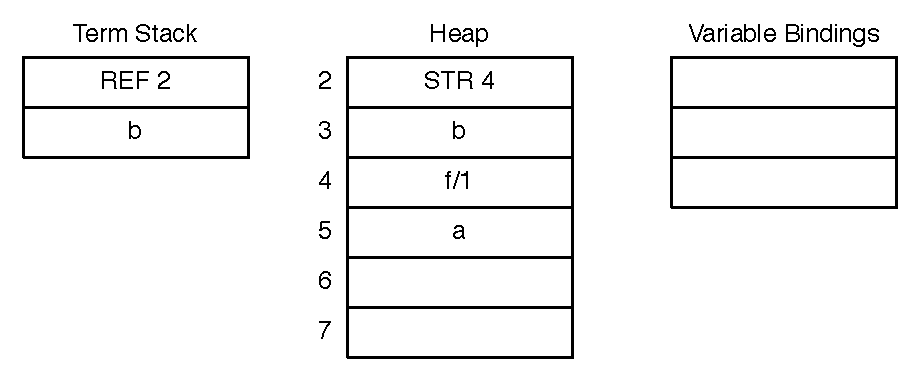
\includegraphics[scale=0.6]{collect_variable3.pdf}
  \caption{After unifying with node (d).}
  \label{fig:collect_variable3}
\end{figure}

Now on the term stack we have \texttt{REF 2}, which dereferences to
a structure on cell 4. On node (e) we have the unbound trie variable
\texttt{VAR0}, which gets bound to \texttt{STR 4} (Figure \ref{fig:collect_variable4}).

\begin{figure}[H]
  \centering
    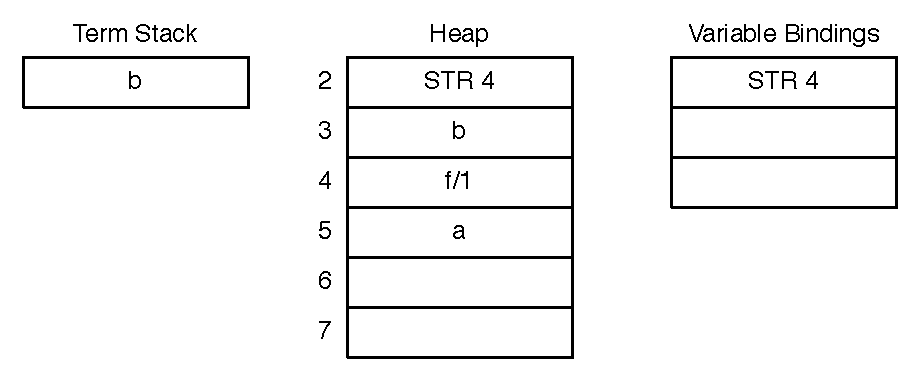
\includegraphics[scale=0.6]{collect_variable4.pdf}
  \caption{After unifying with node (e).}
  \label{fig:collect_variable4}
\end{figure}

Finally, the last term on the term stack is \texttt{b}, which
can not be matched against \texttt{a} on node (f), hence no
relevant answers are found on this trie.

\section{Consuming Answers}

Each consumer subgoal frame stores a linked list with answers that are collected
during evaluation. This list is built incrementally as new answers are generated
for the generator subgoal, which updates the generator time stamp.
Whenever a consumer choice point exhausts the answer list, the retrieval
of relevant answers is attempted so the subgoal frame answer list can be extended.

While the collection of specific answers is done by searching the answer trie
and pruning branches by time stamp and unification failure, it is all done in one
phase. The consumption of a set of answers $S$ is done by consuming one answer $A \in S$
at a time and is completely separated from the collection phase.

Assume we have a trie path from the leaf node $L$ representative of $A$ and
the trie root $R$. Consuming $A$ amounts to unify the symbols on the trie path from $R$ to $L$
to the answer template $AT$ that is built for the consumer choice point. In the end, the variables
on $AT$ are updated so the WAM evaluation branch can proceed with new bindings.

\begin{figure}[H]
  \centering
    \includegraphics[scale=0.6]{consume_answer.pdf}
  \caption{Data structures related to answer consumption.}
  \label{fig:consume_answer}
\end{figure}

As we are certain that $A$ unifies with $AT$, consumption can be reduced to locating a relevant
answer in a trie with only the answer $A$, no time stamp pruning or backtracking is done.
Implementation wise, we use the term stack that is initially pushed with $AT$
and a symbol stack containing symbols from $R$ to $L$. Then, we proceed by
iteratively popping one term from the term stack and one symbol from the symbol stack
and unifying one against the other.

In Figure \ref{fig:consume_answer} we present the data structures involved in consuming
a subsumptive answer. The subsumptive subgoal is \texttt{p(X,Y,Z)} and the
subsumed subgoal is \texttt{p(d,p(X),3)}. The answer to consume is \texttt{p(d,f(a),3)}.
After the answer is consumed, the subsumed subgoal gets a new answer: \texttt{X = a}.

\section{Compiled Tries}

\section{Subsumptive YapTab}

\section{Results}



\chapter{Implementation Details}
\chapter{Experimental Results}
\chapter{Conclusions and further work}
  
\renewcommand{\bibname}{References}
\bibliographystyle{alpha}
\bibliography{references}{}

\end{document}